\chapter{Introduction}

%The Internet was created with the idea that any two computers connected to the common network should be able to communicate with each other. In the Internet Protocol, each computer gets assigned an address which is subsequently used for packet routing. %The most common version of the protocol, IPv4, uses a 32-byte address space which is not enough to uniquely identify all devices on the planet.
%To deal with address exhaustion, internet providers were forced to deploy \textit{Network Address Translation (NAT)} which allows a single address to be shared across multiple devices, but also makes it difficult to communicate between devices without using additional trusted servers.

The Internet was created with the idea that any two computers connected to the shared network should be able to communicate with each other. It has also been built on the principles of decentralization, without any central entity having power to take the network down. Yet, 50 years later, we live in the world where most of the services are centralized and user data are stored on the servers owned by a few large profit-oriented companies.

In the recent years, the idea of decentralization has attracted many in the engineering and research community. Since the introduction of cryptocurrencies in the last decade, there have been many discussions on whether we can decentralize other services, such as social media, or web. With the trend of decentralization, applications are shifting from the client-server model to peer-to-peer, which brings many challenges and calls for a new networking stack.

%including Mobile IP, IPSec, and IPv6
% TODO: client-server model, but recently trend is decentralization

This thesis proposes and implements a protocol for peer to peer communication between any two devices. It is implemented as a Kotlin library which can be used on desktop, smartphones, tablets, and IoT devices. It can be used to deploy a truly ubiquitous network overlay which is available anytime and everywhere. The protocol allows any two devices to establish a direct connection by taking advantage of NAT traversal techniques to connect peers behind different types of NATs. When the Internet connection is not available and peers are located in proximity, the connection can be established using Bluetooth Low Energy.

%Peers are addressed by their public keys and their physical addresses at lower layers are abstracted away.

% The protocol makes best effort to connect peers behind NATs. However, in case the connection is not possible, it resorts to a relay protocol. Bandwidth accounting prevents misusing the relay servers and provides incentive for relay operators. The protocol is completely decentralized and does not rely on any central entity.

%This also allows to route messages over multiple transports. For example, a message can be send over Bluetooth and delivered to a user connected over the Internet by using another device a relay.

% To show one of many practical use cases of the protocol, a simple chat messaging application is implemented on top of it. It allows two users to exchange identities in a secure way to prevent MITM attack. Then they can transfer not only text messages, but also images and videos, to demonstrate a binary file transfer.

The robustness of the NAT traversal mechanism has been tested by conducting a connectivity check between devices using the networks of major mobile network operators and home broadband providers in the Netherlands. The mechanism has been shown to capable of establishing a connection in all tested network conditions.

To demonstrate the usage of the library, a decentralized social network with public feeds and private end-to-end encrypted messaging, which allows trustworthy communication insusceptible to the man-in-the-middle attack, has been implemented. To get feedback on the APIs and general usability of the library, 4 teams of MSc students have been asked to develop non-trivial distributed applications on top of it.

Compared to the state of the art solutions, the proposed library combines both nearby and Internet connectivity, does not require any central server, works on a variety of devices under challenging network conditions, and is completely open source.

\iffalse
\fi

\chapter{Problem Description}

Over the last decade, the Internet and online services have become omnipresent in everyday lives of citizens across the world – communication, shopping, transportation, accommodation, or financial services are only some examples of services where most of the economic activity has already shifted to the online world. Most of these services are operated by so-called \textit{Big Tech} \cite{bigtech}, the largest and most dominant companies in the information technology industry – Facebook, Amazon, Google to name a few. In fact, 7 most valuable companies in the world are now tech companies. It seems to be nearly impossible to function in a digital world outside of the ecosystems created by the big tech. For instance, we require permission from Google and Apple to publish software for mobile devices. Their monopoly power means no other meaningful method exists to reach billions of smartphone users with newly created apps.

\section{Antitrust Battle Against Big Tech}

About 2 billion users interact with Facebook every day. It maintains 75\% social media market share. In a truly free market, they would compete by superior features and providing the best services for their customers to increase the consumer welfare. Instead, Facebook has chosen to mislead and exploit consumers and publishers. The evidence discussed in an analysis paper \cite{antitrust} shows that Facebook has for a decade "engaged in a long-term,
integrated, anticompetitive strategy of half-truths about its privacy policies, exclusionary API manipulation, and anticompetitive acquisitions of nascent competitors". It has acquired various competitors such as Instagram (a social network emhasizing photo sharing) and WhatsApp (a widely popular messaging app) for a hefty premium, just to secure its dominance on the market. Because the market is characterized by a strong network effect, it is unlikely to change without a significant regulatory intervention or consumer uprising.

Over the last months, Departement of Justice, Federal Trade Comission, and the European Union have all started investigations of Google, Facebook, Apple, and Amazon over potential illegal anticompetitive behavior. Very recently, in July 2020, hundreds of large businesses united during the \textit{Stop Hate for Profit}\footnote{https://www.stophateforprofit.org/} campaign and paused all advertising on Facebook platforms for a month to signal disagreement with company's practices and policies.

\section{The Rise of Super Apps}

Meanwhile, a new paradigm in smartphone software engineering has emerged from the East. In 2017, Tencent introduced the concept of a super app, an app that bundles an app store and allows to extend its functionality with mini apps. In a short time, 1 million apps have been developed for WeChat, the most popular communication platform in China and it has attracted 200 million daily users. \cite{wechatapps} WeChat now acts as the ultimate app for a Chinese citizen which bundles online messaging, social media, marketplaces, ride-hailing, food delivery, and other services. Last but not least, it offers financial services. In 2018, over 83\% of payments in China were made using mobile payment methods, with WeChat Pay and Alipay having the major share. \cite{chinapayments} While having the complete social graph and most of the real-world interactions in a single app is useful for providing a good user experience, it is also the perfect spy tool. WeChat is operated by Tencent, a big tech company which is essentially owned by the Chinese government. There has been strong evidence that the app is posing significant privacy risks and is being used to spy on its users. \cite{wechatspy}

Inspired by the trend of super apps, other tech leaders seem to follow the trend. Uber has announced its works on a super app which is posed to become "an operating system for everyday life". It will combine food and grocery delivery, and various forms of transportation services. \cite{superuber} The Facebook app already combines not only social media, but also a marketplace, and soon will include mobile payments with the Project Libra which aims to become a new global payment system \footnote{https://libra.org}. Providing integrated experiences and having access to even more user data will further strengthen the power of already too powerful corporations.

% WeChat: messaging, ride-hailing, payments, thousands of mini apps
% Uber: operating system for everyday life – food and grocery delivery, transportation
% ? Facebook: Marketplace, Events, Videos, Pages, Gaming, Messaging, soon payments with Project Libra

% ideas:

% big tech omnipresent services in lives of citizens across the world
% Facebook reinforcing monopolistic position by purchasing WhatsApp and Instagram. no space for competition due to the network effect
% Tencent owned by the Chinese government
% with their money and data, big tech becomes more and more monopolistic
% unethical behavior, potentially misusing and leaking private data
% dictatorship, users usually left with no other option due to the lack of competition and the network effect
% very recently, hundreds of businesses united during Stop Hate for Profit event and stopped advertising on Facebook over the month of July 2020, to signal disagreement with company's practices and policies.
% our desire => monopolies replaced by sustainable Decentralized Autonomous Organizations (DAO)
% providing the ideal user experience => trend towards a superapp
% research question: can we provide a superapp experience similar to WeChat in a completely decentralized and trustless way, without any intermediaries and trusted third parties?

% problem: vendor lock-in, network effect => monopoly => desire for open social network standard to allow adversarial interoperability
% GDPR - ownership of data, data portability - ZIP export sent to e-mail, not really machine readable

% big tech attack - we need permission of Google or Apple to publish software for mobile devices, enforcing rules not different from dictatorship

% violation of end-to-end principle, internet architecture favors client-server architecture

% architectural building blocks
% - identity layer - public keys of friends or businesses you interact with
% - secure end-to-end encrypted and authenticated communication of any message size
% - NAT traversal mechanism for bypassing NAT boxes
% - social-based overlay with automated IP address discovery based on UDP-puncturing capatable DHT
% - distributed append-only database with eventual consistency – TrustChain

% smartphones - dominant method for Internet access for a majority of the world's population
% superapp approach - 1 million mini-apps on WeChat platform

% disruptive ecosystem resilient against attacks by disintermediated corporate entities
% - legal intimidation, layer-based attacks and creation of chilling effects
% - ownership by everybody and nobody
% - anyone can create and distribute a miniapp, self-moderation left solely on community, no centralized arbiters of truth

% evaluation: 4 master student teams developed non-trivial distributed apps on top of our foundational architecture within 10 weeks: online voting, shared ownership of money, distributed marketplace

% proof of principle: zero-server based messenger and social network

% Spotify alternative disrupting music industry by removing middlemen in the distribution process, money goes directly to artists, a project evolved into a separate thesis


% trust built into platforms with no interoperable standard

%
% The Internet standards are developed by the working groups of Internet Engineering Task Force (IETF), a non-profit open standards organization composed of volunteers. Its evolution is based on a rough consensus about technical proposals, and on running code. While there are many conflicting opinions on its architecture, the general consensus is that the main goal of the Internet is to provide global connectivity by the \textit{Internet Protocol (IP)}. \cite{internetarchitecture} This ultimate goal requires cooperation of multiple parties, including researchers, developers, and commercial service providers.


% In an ideal world, there would be only one protocol on the Internet level to facilitate seamless integration between service providers, hardware manufacturers, and application developers. However, in practice, multiple protocols need to be supported by the network at the same time, e.g. during periods of transitioning to a newer version of IP.

\section{End-to-End Principle Challenged}

The architecture of the Internet has emerged in an evolutionary process rather than from a carefully designed grand plan. There is no central entity in charge of architectural decisions, or anyone with ability to turn it off. Most decisions related to protocol and system design have for a long time followed the \textit{end-to-end principle}, which states: "The function in question can completely and correctly be implemented only with the knowledge and help of the application standing at the end points of the communication system. Therefore, providing that questioned function as a feature of the communication system itself is not possible." \cite{endtoend}

It implies that the job of the network should be merely to deliver datagrams as efficiently as possible, and the rest of the responsibilities should be pushed to the end points of the communication system. As every application has different requirements, providing additional features on the Internet layer would turn some applications not using those features less efficient. It is also cheaper to upgrade the end points to add new capabilities rather than replace the network infrastructure. A common example for supporting the end-to-end principle are delivery guarantees. In the ARPANET, the receipient would send \textit{Request For Next Message} packet every time a packet was delivered. However, some applications would still need to implement its own acknowledgements on the application level, to indicate that the messages were processed correctly. Similar examples can be found for supporting authentication, encryption, and other guarantees in communication systems.

The end-to-end principle has been challenged by introduction of \textit{middleboxes}, intermediary nodes in the network that perform functions different from functions of a regular IP router. In \cite{rfc3234}, an extensive catalogue of 22 different middlebox classes has been analyzed. Network address translators (NATs), packet classifiers, IP firewalls, application layer gateways, or proxies are just a few examples of components hidden in the network. While most of them try to be transparent, the behavior of certain middleboxes can severly impact the end-to-end performance, either by delaying packet retransmission, or aborting user sessions entirely in case they crash. Some of them perform advanced logic on different protocol layers and keep a hard state, which violates the end-to-end principle stating that the network should be kept as simple as possible.

% \section{Overcoming Address Exhaustion}

In the Internet Protocol, each computer gets assigned an address which is subsequently used for packet routing. The most common version of the protocol, IPv4, uses a 32-byte address space which is not enough to uniquely identify all devices on the planet. To deal with IPv4 address exhaustion, internet providers were forced to deploy different types of NATs which allows a single address to be shared across multiple devices.

Traditionally, each consumer would have a NAT implemented in the router located at the edge of the network. It would serve as a gateway between the local area network (LAN) and the wide area network (WAN), the Internet. This type of NAT usually maps all addresses inside LAN to a single external WAN address. It also provides additional features such as firewall, which only allows incoming traffic on ports that are explicitly open, or on whose the client initiated the communication first.

% TODO: Decide whether to stay here or in state of the art

However, to further conserve the address space, and facilitate transitions to IPv6 with backwards compatibility of IPv4, it has become a trend among internet service providers to implement a NAT in their infrastructure. This topology is called a \textit{carrier-grade NAT} (CGN). Carrier-grade NAT is by definition managed by the network operator and the customer does not have any control over it. CGN usually implement a complex functionality to ensure reliability for thousands subscribers and compliance with legal regulations, which again violates the end-to-end principle. Inability to manage open ports breaks the communication model of many peer-to-peer applications which usually have to reside to using a proxy server for relaying communication.

To mitigate this issue, \textit{Port Control Protocol (PCP)} \cite{pcp} has been designed and recommended by IEFT to enable port forwarding in CGN deployments. However, our experiments have shown that most providers do not have this mechanism deployed at the moment and that some providers have deployed a version of CGN that does not satisfy NAT behavioral requirements \cite{behave}, which makes P2P communication nearly impossible.

%\section{Ubiquitous Overlay Network}

%\section{Net Neturality Under Attack}

\section{Freedom of Trustworthy Communication}

The principle of network neutrality states that ISPs must treat all traffic equally and not discriminate based on its content, addresses of recipients, or methods of communication. However, we can see that this principle is violated in many cases, some of them more worrying than others. There are several countries that enforce Internet censorship either by simple IP address blocking, or advanced deep packet inspection, preventing people from communicating freely.

Even in places with relatively mature infrastructure, there are occasionally connectivity issues at places with high gatherings of people, such as conferences or festivals, causing congestion in the infrastructure networks. The increasing capabilities of smartphones and novel wireless networking technologies open up possibilities to a whole new range of applications that can communicate without the need for the Internet connection. The ideal communication protocol should be able to use those when possible. It has been seen how the Bluetooth technology can be useful in creating a mesh network during the Hong Kong protests in 2018 and 2019, where protesters relied on peer-to-peer communication apps as a communication tactic.

Another problem related to communication is ensuring message authenticity and privacy. Most of the commonly used protocols have adopted \textit{Transport Layer Security (TLS)} protocol to secure all communication between clients and servers. The trust in the system is enforced by using \textit{public key infrastructure (PKI)} with trusted certificate authorities. However, public key infrastructure is not easy to adopt to a peer-to-peer system with self-sovereign identities.

\iffalse
\section{Re-decentralization of Internet Infrastructure}

While the Internet is built on the principles of decentralization from the ground up, we cannot say so about the Web and other services built on top of it. The majority of the websites is operated by a few hosting companies and most of the static content is served by a few \textit{Content Delivery Networks (CDNs)}. For example, \textit{Cloudflare} currently powers 10 \% of all internet traffic\footnote{https://blog.cloudflare.com/cloudflare-traffic/}. Since there is a central point of failure, if a provider experiences outage, a large part of the internet goes down.

The inventor of the World Wide Web has proposed a Solid \cite{solid} as an architectural pattern for building the next generation of decentralized social applications. It is based on the principle that users own their data and have freedom of choice where to store them, which significantly improves privacy and data reusability. As the application logic is decoupled from the data storage servers, multiple applications can access them same data if allowed by the user.

\fi

\section{Research Focus}

While it is out of scope of this thesis to provide the complete solution for the next generation of web applications, the afore-mentioned problems and challenges lead us to the following question:

\begin{displayquote}
\textbf{How can we create a self-organizing technology stack that would allow to build decentralized alternatives of the services currently provided by the big tech companies?}
\end{displayquote}

Our work consists of 2 parts. First, we design a zero-server architecture and develop several networking primitives which remove the need for central control by any trusted third party. No central element exists which can form a performance bottleneck or point-of-failure. These serve as the basic building blocks for creating full fledged Facebook alternative with full interoperability and data portability. We have not created a full alternative to Facebook within the context of a single master thesis. However, we provide the basis for it and claim that our infrastructure will scale to usage by the 2 billion existing Facebook users without fundamental alterations. Our Internet-deployed network primitives are:

\begin{itemize}
    \item Identity layer based on public keys of trusted contacts with secure public key exchange
    \item Authenticated communication bypassing NAT boxes and other imperfect hardware
    \item Establishing connection with known contacts using a social-based zero-server overlay with automated Internet address discovery based on a UDP-puncturing capable DHT
    \item Secure end-to-end encrypted messaging of any message size
    \item Distributed bookkeeping with tamper-resilience using TrustChain to synchronize data, prevent spam and abuse
\end{itemize}

\iffalse
Our zero-server architecture is also meticulously designed to offer another unique property: resilience against legal attacks. Legal action may be expected when a monopoly is attacked. We believe that this thesis proves the first proof-of-principle of a disruptive open innovation ecosystem which is resilient against attacks by disrupted or disintermediated corporate entities. Possible legal attacks includes: legal intimidation, lawyer-based attacks and creation of chilling effects. Our unique approach to governance gives ownership to both nobody and everybody. By creating an academically pure form of self-organisation we create a leaderless infrastructure in which even the original creators have no special powers. It is difficult to block, disrupt or shutdown our zero-server approach with either legal or technological means when used by citizens at scale.
\fi

We then take advantage of these building blocks to build our own decentralized version of a super app with ability to extend its features using mini-apps. The first version of a distributed social network with private messaging and a public feed has been developed as the proof of principle that service like Facebook could potentially be built using this stack.
%On top of our networking primitives we facilitate an open innovation ecosystem.
%Every user can extend the functionality of the platform freely. No gatekeepers exists to moderate mini-apps, this relies on self-moderation by the community.

We also conducted an experiment around the mini-apps to determine how easy they are to develop. Various student development teams with 17 members in total successfully created various mini-apps with our zero-server architecture. Developed mini-apps within a 10-week period include: group creation and shared ownership of money, secure online quorum-based voting, decentralised machine learning, and sharing of music records. The music sharing app has grown into another full master thesis aiming to remove all proprietary infrastructure between artists and ears of listeners with a cost-free ecosystem.

\iffalse
We analyze the question in more detail:
\begin{itemize}
    \item The communication should be \textbf{trustworthy}, which means we can verify that we received the message from the person that claims to be its sender. The communication can be optionally encrypted to provide privacy on top of authenticity.
    \item The communication should be facilitated \textbf{device-to-device} without need for any additional \textbf{server} infrastructure, with the exception of the initial bootstrap server. The bootstrap server should not be needed if there are peers in proximity which can be used for bootstrapping.
    \item The protocol should be able to work under \textbf{challenging network conditions}, which means it should be robust against the presence of various middleboxes. Mainly, it should be able to establish connection in presence of carrier-grade NATs deployed by mobile network operators.
    \item The communication protocol should in theory work on both most popular \textbf{smartphone} operating systems and support their most commonly used versions. However, supporting only the most commonly used OS would be sufficient for the prototype.
\end{itemize}
\fi

% TODO: mention SOLID

% history of internet, IPv4
% address exhaustion, mobility

% NAT breaks end-to-end principle
% solutions:
% - IPv6
% - Mobile IP
% - IPSec
% IPv6 still not widely deployed
% - TU preparing for IPv6 since 2012
% - not available on any cellular network in NL

% motivation for decentralized internet
% problems with current internet:
% - censorship
% - data in control of big companies
% we need building blocks to disrupt centralized services
% data in controls of users
% first steps: connectivity, data availability, privacy
% mention blockchain as enabler of permissionless economic activity

% ubiquitous overlay
% - peer to peer connectivity over the Internet
% - off-grid communication without internet access

% research question: How to establish a secure connection between two smartphone devices without using a central server?


\chapter{State of the Art}

% TODO: better reasoning why we are researching these topics

In this chapter, we conduct a short survey of various topics related to P2P communication. We start by analyzing existing solutions and platforms for decentralized communication. We continue by introducing the problem of network address translation (NAT) and commonly used solutions for fixing the broken internet infrastructure by techniques known as NAT traversal. Finally, we introduce wireless communication technologies provided by modern smartphone devices and analyze them based on practical usability for infrastructureless communication.

\section{Decentralized Communication Platforms}

In general, we can divide platforms into three classes based on their architecture and degree of decentralization. The traditional \textit{centralized} platforms such as Twitter, Facebook, and Instagram are operated by large prof-oriented companies. All data are stored in data silos owned by those companies and used for targeting advertisements and other marketing purposes.

\textit{Decentralized} platforms, where everyone usually runs their own node and is completely in control of their data. There are many projects dealing with the problem of peer to peer (P2P) communication on different levels, ranging from general-purpose libraries that can be used to build applications (libp2p, IPv8), to feature-packed platforms providing social networking features on top of their custom-designed protocols (Briar, Bridgefy, Berty, Secure Scuttlebutt). We try to analyze their functionality from the technical and usability perspective, state their advantages and shortcomings, and propose improvements when possible.

\textit{Federated} platforms represent the middle ground between completely centralized and decentralized platforms. They consist of an ensemble of interconnected servers that communicate with each other using open protocols.

\subsection{Fediverse}

Fediverse is an ensemble of interconnected servers that run open-source social networks and communicate with each other. Historically, there are many open protocols for social networking including diaspora, OStatus, DFRN and many projects built on top of them. In 2018, the World Wide Web Consorcium presented the ActivityPub protocol aming to improve interoperability between platforms. Some of the most common platforms implementing this protocol are Friendica, Mastodon, or PeerTube.

\begin{figure}
    \centering
    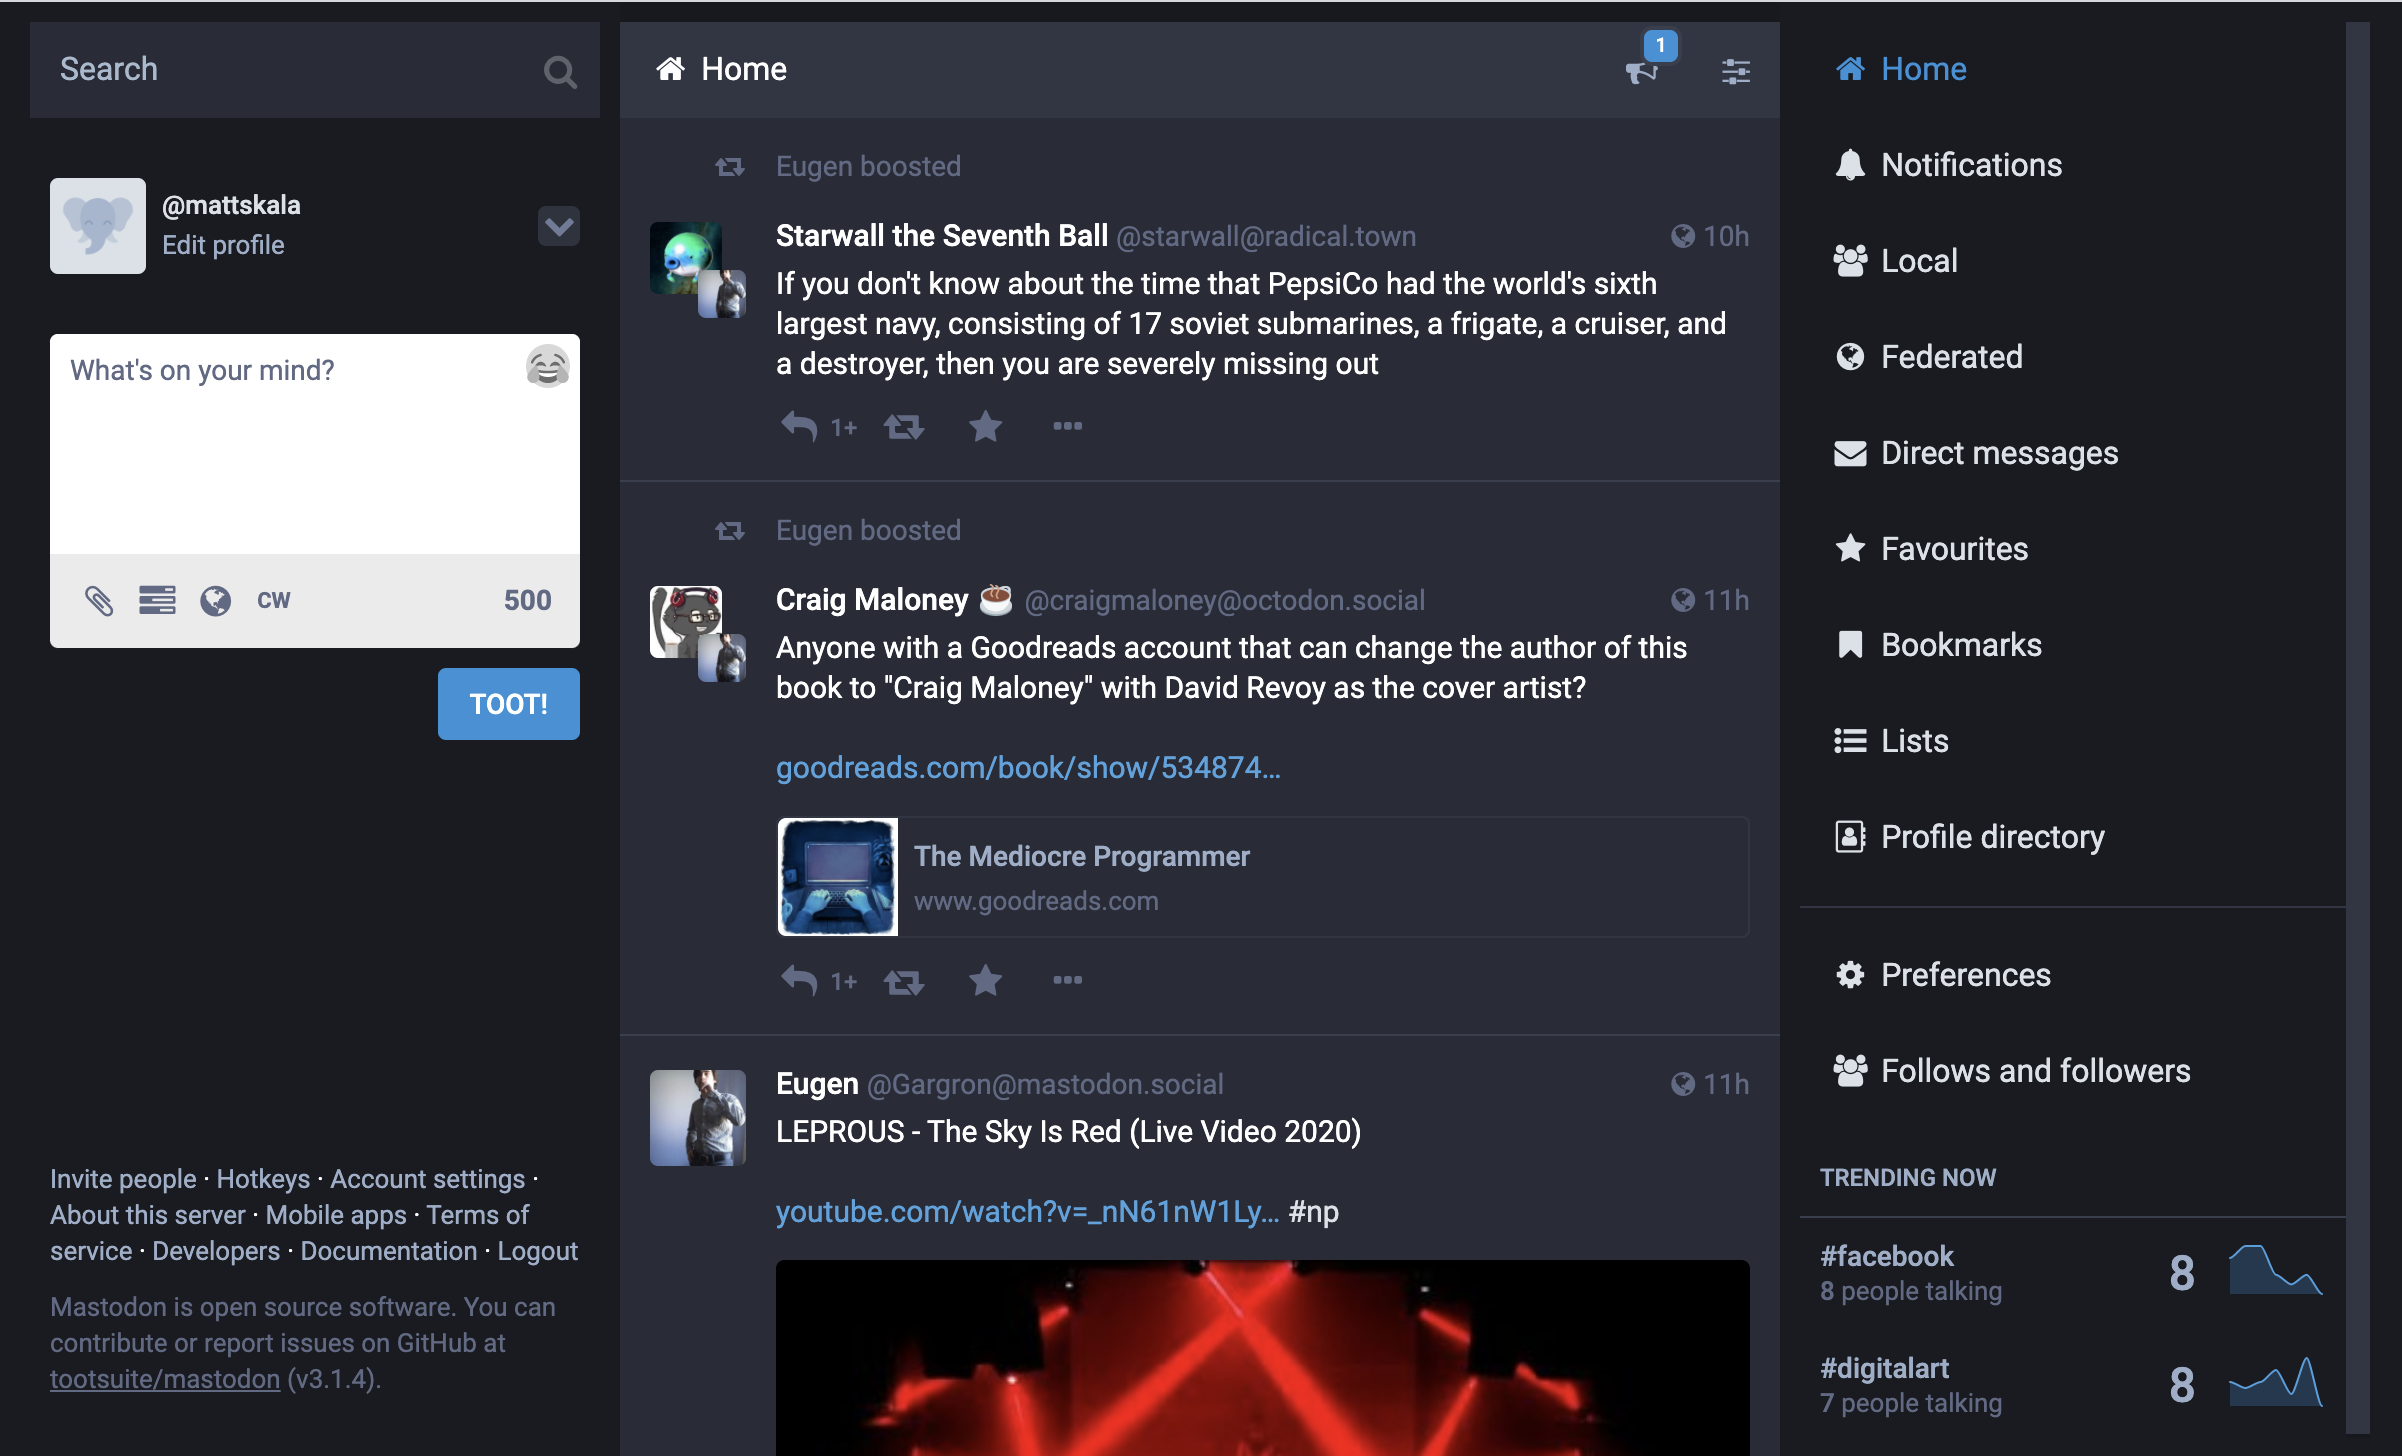
\includegraphics[width=\textwidth]{screens/mastodon}
    \caption{The screenshot of mastodon.social, an example of a federated social network}
    \label{manyverse}
\end{figure}

In contrast to mainstream social platforms, federated networks are developed by communities of people, independent from any corporation. Anyone can run its own Fediverse server, and users have to choose the operator through which they are connecting to the network. As this improves privacy by open source protocol, users still have to some extent trust their server operators. There is usually a lack of incentivization for server operators. Some operators charge a fee for joining the network to fund their operation, which however contradicts the freedom of communication.

\subsection{libp2p}

% TODO: libp2p stack

libp2p\footnote{https://libp2p.io} is a modularized peer-to-peer networking stack and library. It is being developed by Protocol Labs, a non-profit company behind the Interplanetary File System (IPFS)\footnote{https://ipfs.io}, a distributed filesystem combinig some fundamental ideas from BitTorrent and Git. They extracted the networking logic from the IPFS project into a library after realizing it could be useful for other applications as well. It is to date probably the most widely known universal P2P library. It was originally implemented in Go and JavaScript, and there are ongoing efforts to provide implementations in Rust, Haskell, Kotlin, and Python. One of the promises of the Kotlin implementation will be the ability to run it natively both on JVM and Android runtime.

The library is composed of several layers, where each can be implemented by one of interchangeable modules. It is presented as a collection of peer-to-peer protocols for finding peers, connecting to them for finding content, and transferring it. It implements port mapping and hole punching inspired by STUN to deal with NATs. The \textit{identify} protocol allows nodes to discover their public address and the \textit{AutoNAT} service allows them to discover the NAT behavior by forcing other peers in the network to attempt to connect to them. When the NAT traversal fails, there is a circuit relay protocol that allows peers to communicate indirectly using intermediate peers, which similar to the functionality of TURN servers. Currently, the relay protocol requires a list of relays to connect to. An \textit{autorelay} protocol for discovering public relays is under active development. \textit{Kademlia DHT} is used as a primary mechanism for peer routing, i.e. finding routable addresses of peers based on their public keys.

% \subsection{Nearby Connections API}

% \subsection{MultipeerConnectivity}

% \subsection{Bridgefy}

\subsection{Briar}

% TODO: Better description

Briar \cite{briar_gplay} is an open-source project which aims to support freedom of expression and right to privacy. It enables peer-to-peer encrypted messaging and forums. It is presented as a tool for activists, journalists, and anyone who needs a safe way to communicate.

\begin{figure}
    \centering
    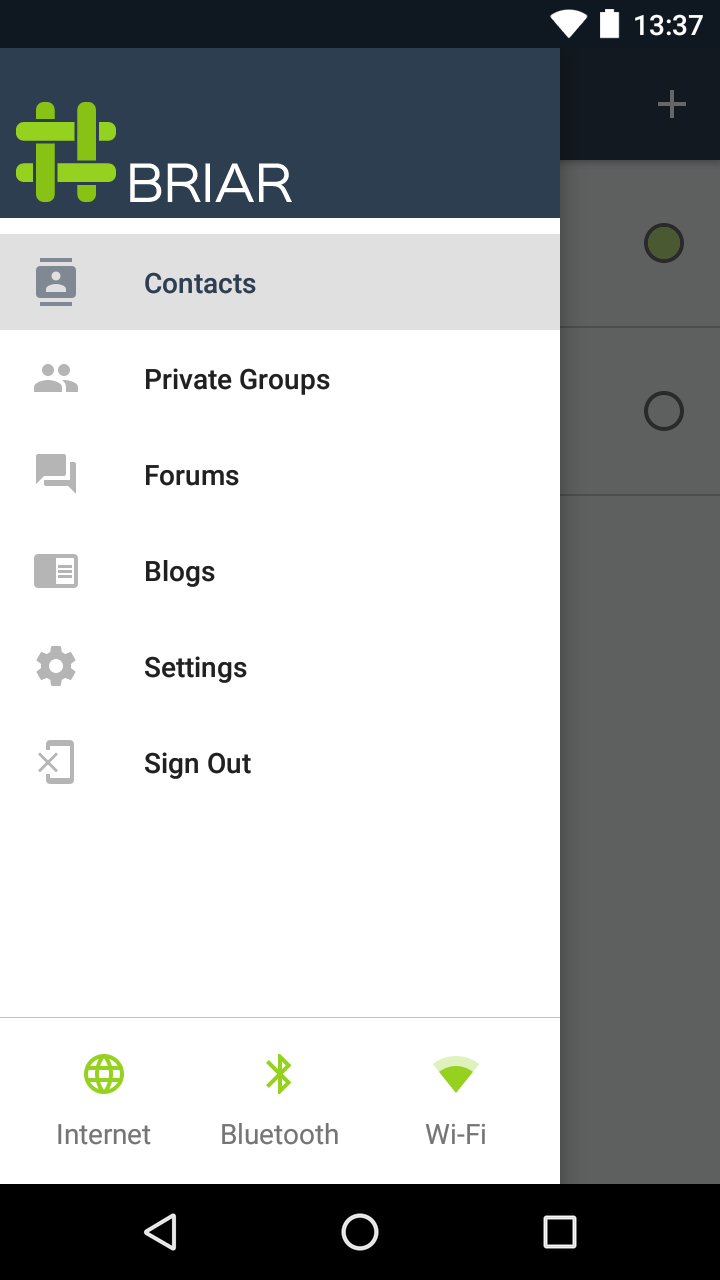
\includegraphics[width=0.32\textwidth]{screens/briar/briar1}
    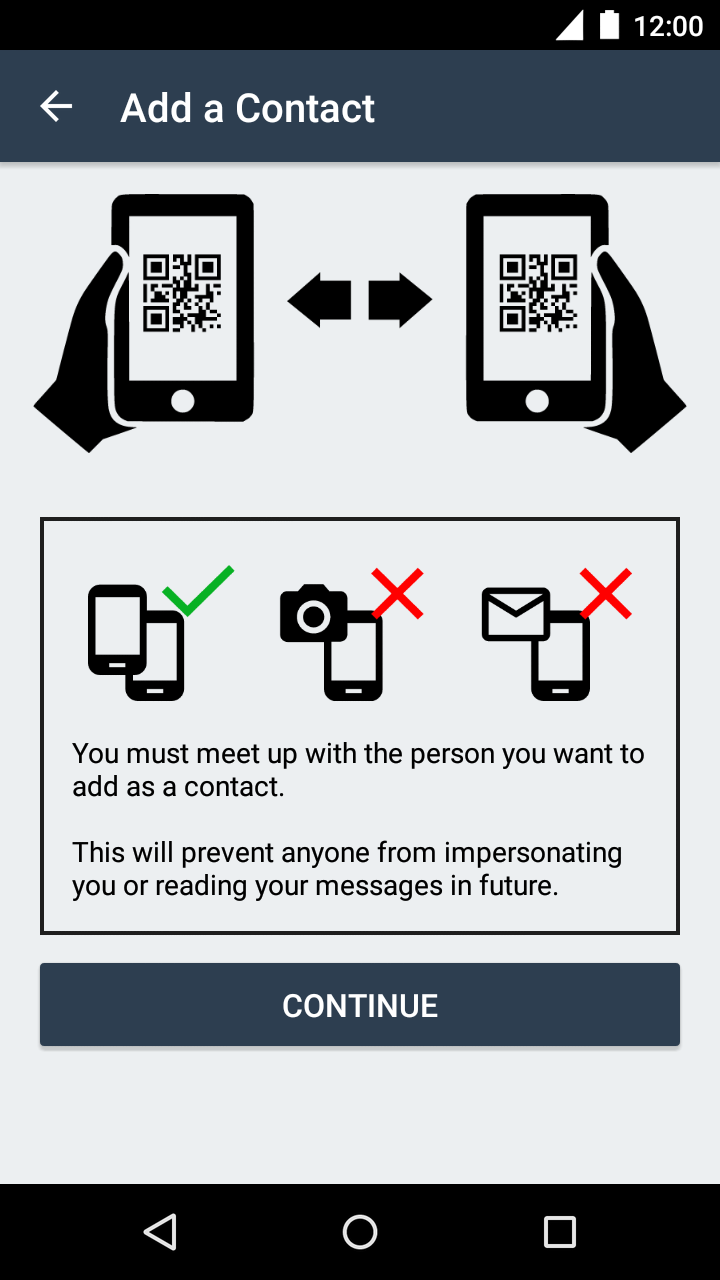
\includegraphics[width=0.32\textwidth]{screens/briar/contact}
    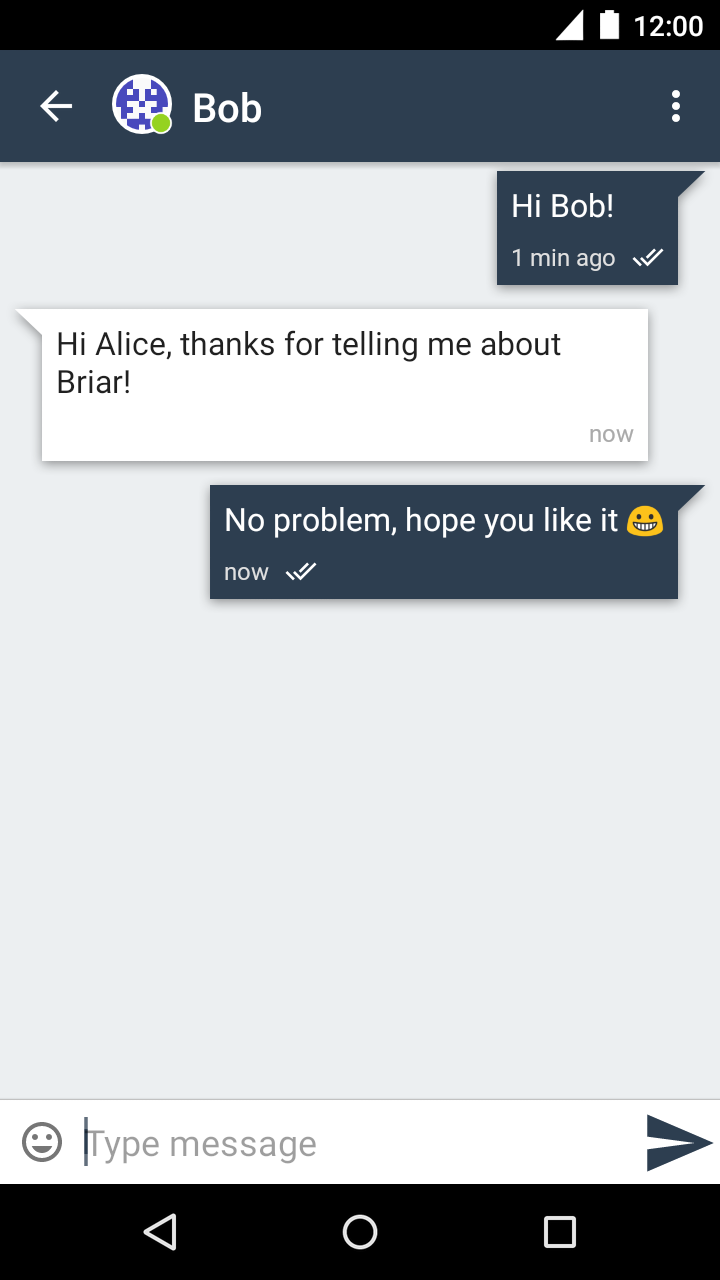
\includegraphics[width=0.32\textwidth]{screens/briar/briar2}
    \caption{The menu, contact exchange, and the conversation detail in the Briar app}
    \label{manyverse}
\end{figure}

Before the communication starts, users have to meet in person and scan QR codes from each other's screen. The devices exchange public keys and agree on a shared key using \textit{Bramble QR Code Protocol (BQP)} \cite{briar_bqp}.
%The protocol requires both devices to have Bluetooth enabled and be discoverable, or be connected to the same WiFi network.
This provides strong identities secure against man-in-the-middle attacks.
The device only accepts connections from devices in contacts. However, the user can initiate an introduction between two of her contacts. If both contacts accept the introduction request, then they are able to establish connections without meeting in person.

The communication is built on top \textit{Bramble Transport Protocol (BTP)} and \textit{Bramble Synchronization Protocol (BSP)}, transport and application layer protocols suitable for \textit{delay-tolerant networks}. \cite{briar_stack} It does not rely on any central server, but instead allows to synchronize messages using Bluetooth or Wi-Fi. If the Internet is available, it can also connect via the Tor network.

% \subsection{Berty Protocol}

\subsection{Secure Scuttlebutt}

Scure Scuttlebutt (SSB) \cite{ssb} is a peer-to-peer gossip protocol for building decentralized applications. Its first application was a distributed social networking platform Scuttlebutt. Each peer in the network has its own identity generated from its public key. Every identity is tied to its own feed, which is represented by an append-only log of messages. Each message is signed with the peer's private key to provide authenticity. Every message also has a pointer to the hash of the previous item in the log, which helps to ensure data integrity during replication.

\begin{figure}
    \centering
    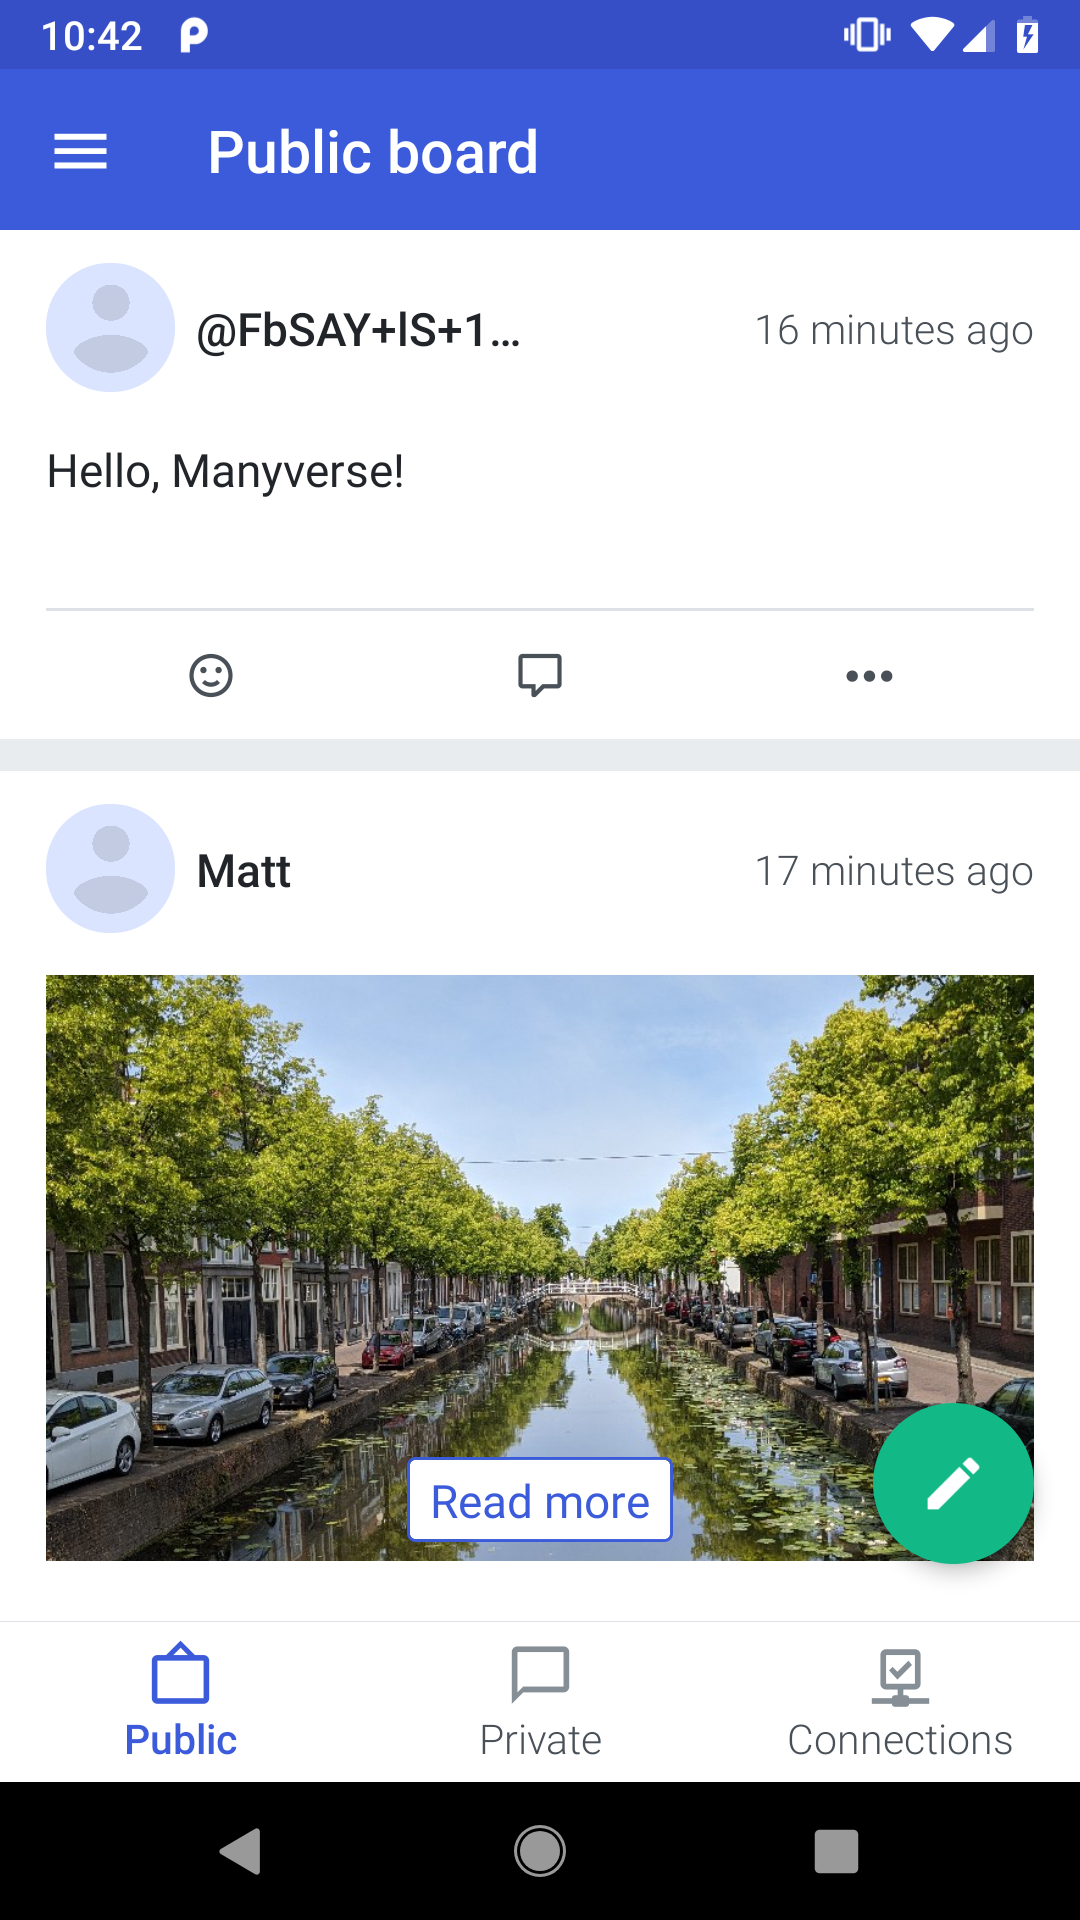
\includegraphics[width=0.32\textwidth]{screens/ssb/feed}
    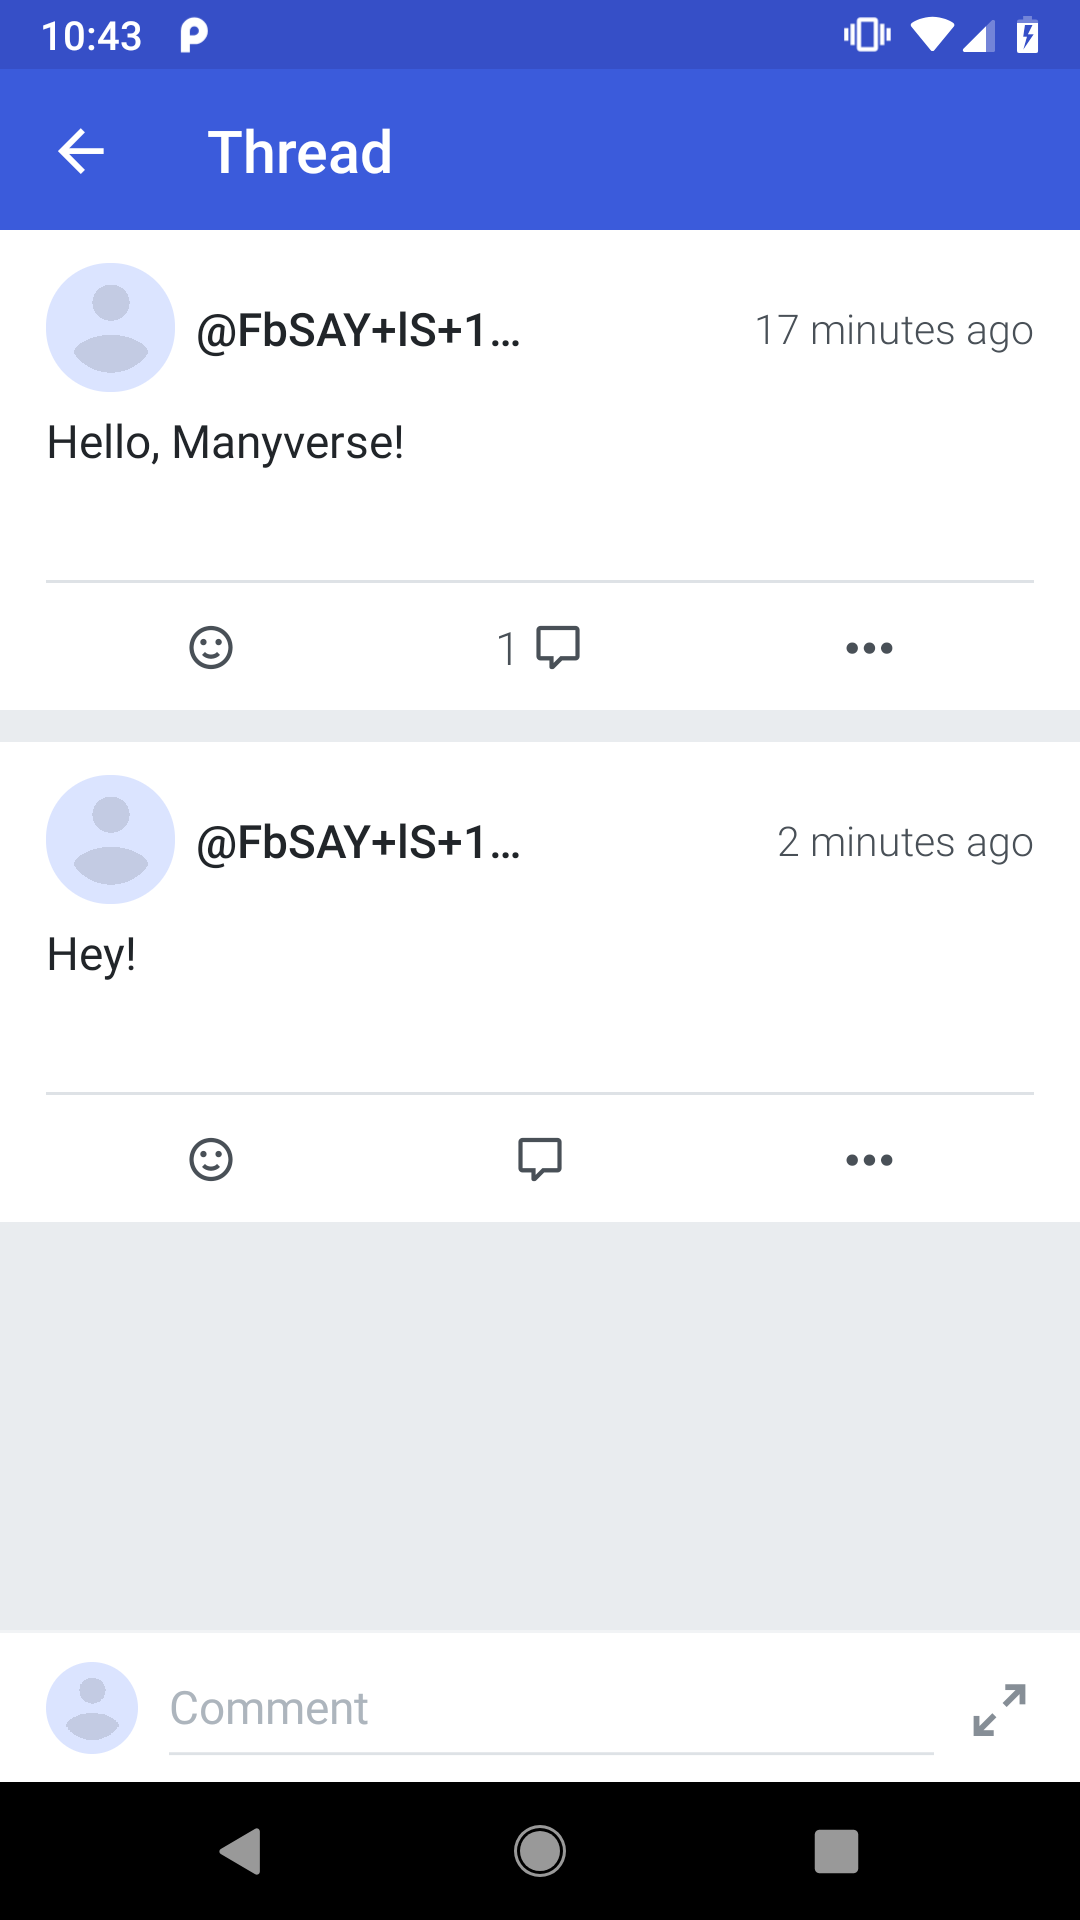
\includegraphics[width=0.32\textwidth]{screens/ssb/thread}
    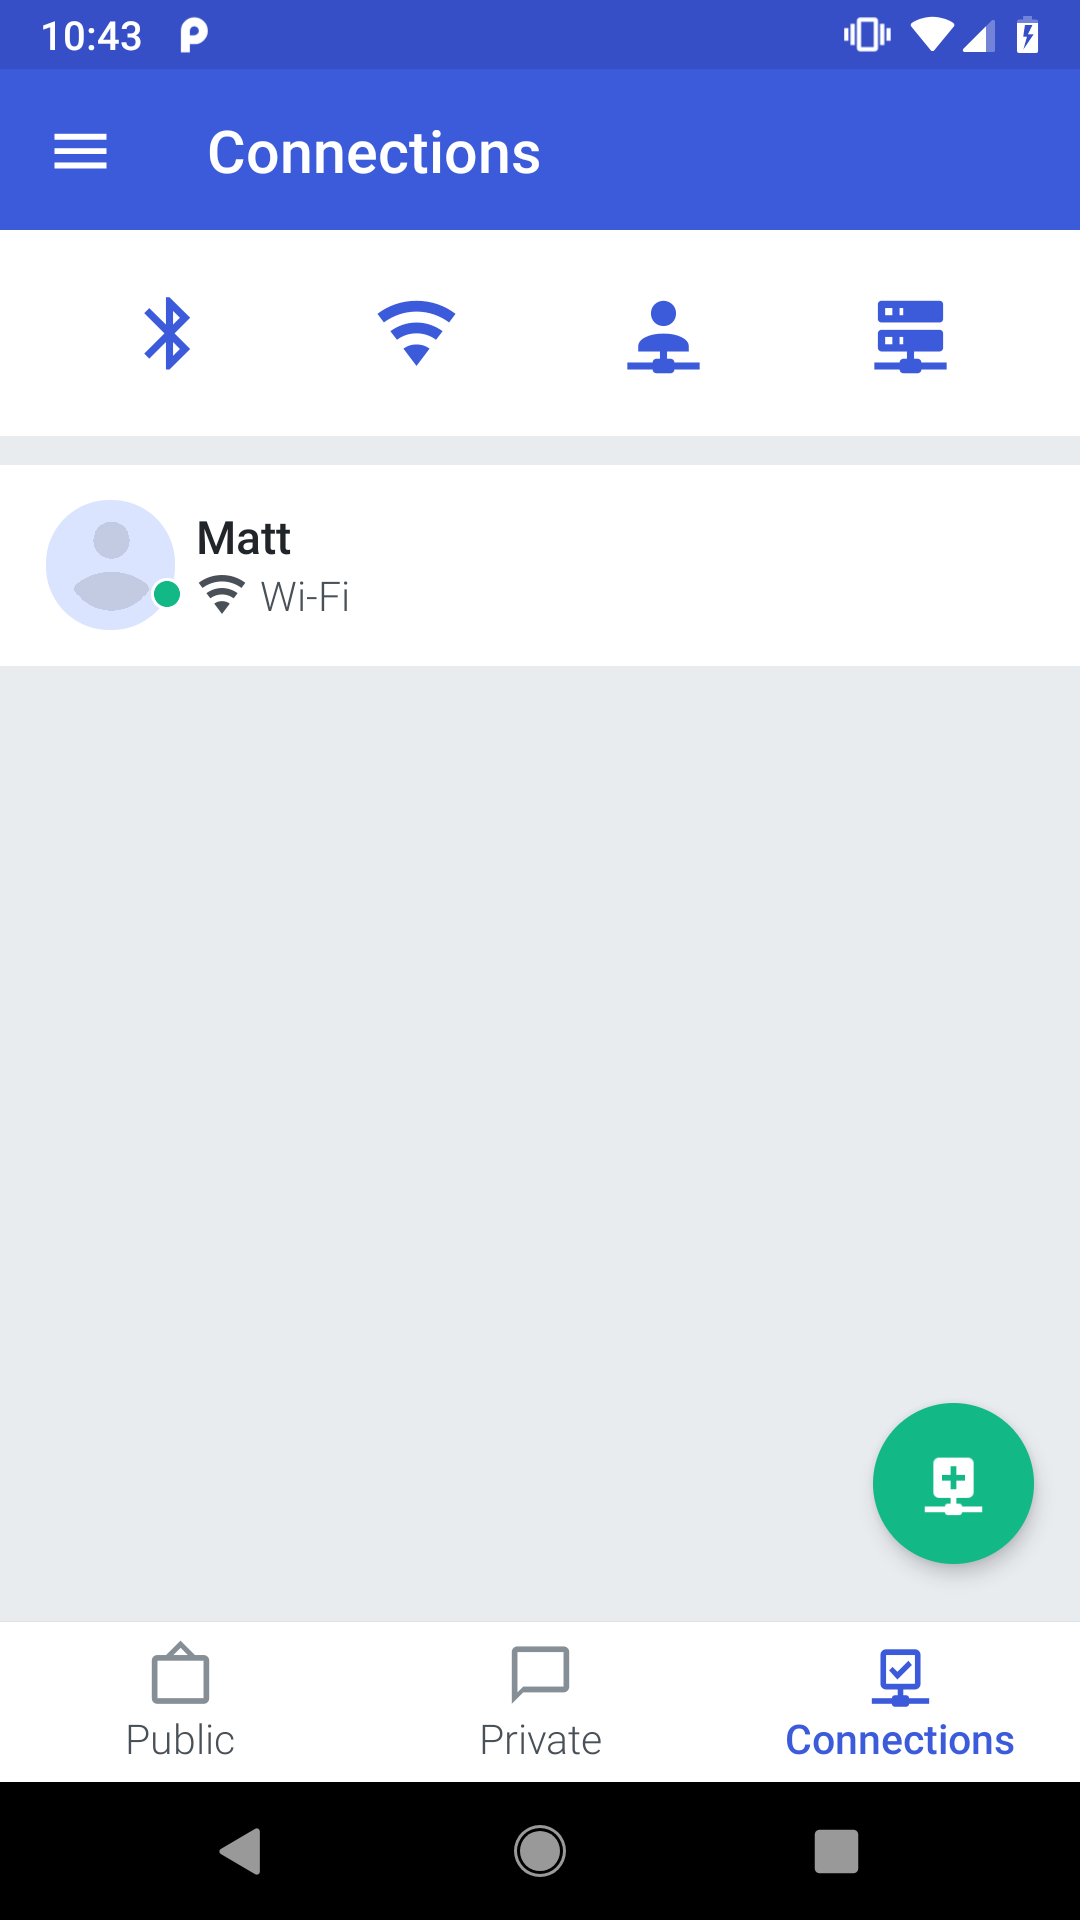
\includegraphics[width=0.32\textwidth]{screens/ssb/connections}
    \caption{The feed, thread, and connections list UI in the Manyverse Android app}
    \label{manyverse}
\end{figure}

The system architecture is designed to be completely decentralized and work off-grid without any infrastructure. Each peer stores its entire feed history and feeds received from other peers. When peers get connected, they exchange their feeds and feeds of people they follow. The protocol provides eventual consistency.

\subsubsection{Peer Discovery}

The protocol can perform peer discovery either by UDP broadcasting over the local area network, or more commonly, by using \textit{pubs}. A pub is a peer which is publicly accessible on the Internet. The user who wants to join the network first needs to obtain an \textit{invite link} containing the IP addres, port, and a public key of a pub. The peer establishes a connection with the pub over TCP using the Secret Handshake key exchange \cite{secrethandshake}. Subsequently, they can communicate using an RPC protocol. The peer can then access feeds of other peers followed by the same pub.

\subsubsection{Blobs}

Messages can contain links to binary large objects, or \textit{blobs}. Peers send to each other lists of blobs they \textit{have} and \textit{want}, in a similar fashion as in the BitTorrent protocol. Peers can also download blobs on behalf of each other if any of their peers have the blob requested by another peer, to increase data availability. The blobs are addressed by hashes, so anyone who fetches them can verify they have not been tampered with.

\subsubsection{Private Messages}

Sometines the user wants to send a private message that can be read only by one or more specific people. In that case, the message needs to be encrypted in a way that it can be decrypted only with people owning the corresponding private keys. For each private message, the sender generates a random secret key to encrypt its content. The sender then encrypts the secret key with a public key of each recipient of the message and includes these encrypted keys in the message header. The identity of recipients is not revealed. Instead, every peer who receives the message has to try to decrypt the key to find out if they are one of the intended recipients.

\subsubsection{Conclusion}

The reference protocol implementation is written in Node.js, with ongoing efforts for Go, Python, and Rust implementations. There is an official multiplatform UI client Patchwork\footnote{https://scuttlebutt.nz/} implemented in the Electron framework. There is also a mobile client called Manyverse\footnote{https://www.manyver.se/} written in React Native, available both for Android and iOS.

While the protocol claims to be peer-to-peer, it is based on client-server communication model, as most of the communication happens via publicly available peers called pubs. There is no NAT traversal layer, so peers behind NATs are not able to communicate with each other directly. We are also questioning the scalability and incentive alignments of the protocol, as users are by default supposed to store complete feeds and blobs even for friends-of-friends. Also, all private messages are stored in the public feed and replicated across many peers, even when the message can only be decrypted by a single peer, which creates unnecessary overhead.

\subsection{IPv8}

IPv8 \cite{ipv8} is a P2P networking library developed over the last 13 years at TU Delft. It is an evolution of previous generations of \textit{BuddyCast} \cite{buddycast} and \textit{Dispersy} \cite{dispersy}. Its primary purpose is to serve as the networking layer of Tribler, an anonymous P2P file-sharing client. However, it attempts to be a general-purpose library which can be used to build custom P2P overlays and applications. It is conceptually composed of several layers:

\subsubsection{Identity}
The identity layer provides each peer with a private and public key pair. This allows authenticated communication. The public keys can also be used for addressing and IP addresses are ultimately abstracted away.

\subsubsection{NAT Traversal}
UDP hole punching is implemented as a basic NAT traversal technique to allow connectivity between peers behind NATs.

\subsubsection{Peer Discovery}
Discovery protocol based on a \textit{distributed hash table (DHT)} allows to connect to specific peers using their public key, without need for knowing their IP address. While there is a list of trusted bootstrap servers provided, in theory any peer in the network can be used to bootstrap connection, thanks to distributed nature of UDP hole punching protocol which does not rely on STUN servers.

\subsubsection{TrustChain}
The library also provides TrustChain \cite{trustchain}, a scalable distributed ledger for tamper-proof accounting. It is currently mainly used as a bandwidth accounting mechanism to prevent freeriding in Tribler, but has wide range of other potential use cases, including a decentralized asset exchange \cite{anydex}, or identity attestations and verifiable claims.

%\subsubsection{Known Issues}
%There are several known issues with the current implementation of the library, which we now briefly discuss.
%\begin{itemize}
%Firstly, the communication is based on UDP and no higher-level transport protocols are supported. This means it is a responsibility of a developer that all messages fit into a UDP packet.

%Currently, only IPv4 addresses are supported, while adding IPv6 support is planned for future updates. However, there still problem with testing infrastructure, as IPv6 has been coming to TU Delft since 2012 and still is not fully deployed.

%The library works for establishing connections between computers on the public Internet, but starts to behave unpredicatbly when some of the peers are on the same LAN. Firstly, it uses public addresses for communication and thus relies on the NAT to support hairpinning, which is not always the case. When LAN connection is established using a LAN address, the connectivity can break because the peer starts to confuse its LAN address with a public address due to insufficient robustness of the UNSAF mechanism.

%UDP hole punching is only effective for NATs implementing endpoint independent mapping. Peers behind NATs with more complex behavior are usually not connectable. However, this is remedied by the tunneling which allows to use other peers as proxies.

\subsubsection{Mobile Support}

It is written in Python, as well as the rest of the Tribler stack. While using a single language during the whole development process is convenient for the Tribler team, the language choice has been a limiting factor when porting to mobile platforms such as Android. There have been attempts to run IPv8 on Android using \textit{python-for-android}\footnote{https://github.com/kivy/python-for-android} toolkit which allows to build a Python interpreter together with the application source code into an APK. However, the whole build process has shown to be fragile and impractical. Firstly, the build of the whole library takes almost an hour, which severely degrades developer experience and slows down iterative development. Secondly, it has turned out to be problematic to compile a 64-bit APK that would comply with the requirements for publishing on Google Play.

There has been a long track of efforts to explore the usage of mobile devices in peer to peer systems at TU Delft. The \textbf{app-to-app communicator}\footnote{https://github.com/Tribler/app-to-app-communicator} was an early prototype that implemented a basic UDP hole punching method to test the feasibility of a device to device overlay without any server infrastructure. The \textbf{self-compiling Android application}\footnote{https://github.com/Tribler/self-compile-Android} was an experimental project that bundled all tools from the Android SDK required to assemble an APK on Android. This has proven viability of trustworthy code execution without dependency on a centralized app store. The \textbf{trustchain-android}\footnote{https://github.com/Tribler/trustchain-android} project implements a TrustChain-like distributed ledger and a UDP hole punching protocol. It has been written in Java, but the protocol is not compatible with TrustChain which was originally implemented as part of the py-ipv8 library, even though it uses the same principles. %In this thesis, we will build on top of this existing research, but with usage of modern tools available today.

\section{Network Address Translation}

\textit{Network Address Translation} (NAT) is a method of mapping addresses from one address space into another by modifying the IP header of a packet on its way from the source to the destination. It has been originally proposed as a temporary solution to slow down IPv4 address space exhaustion, until a better solution is implemented. \cite{nat} Yet, it has become so ubiquitous in the Internet infrastructure that almost all end users are located behind a NAT nowadays.

NAT is designed to be fully transparent when using the client–server communication model. However, it creates major obstacles to peer-to-peer and VoIP applications, where end user devices need to establish direct connections without using a third-party server. This topic has been estensively researched and still, fragile workarounds are required to support direct communication between users behind NAT boxes. This hurdle could be one of the reasons why the server-centric model, which deviates from the original ideology of the Internet, has prevailed in most of the services we use today.

\subsection{NAT Classification}
\label{nat-classification}

% TODO: image of NAT classifiction

The original proposal did not specify the exact behavioral requirements of a NAT, so hardware manufacturers had to decide a lot of implementation details on their own. This has resulted in fragmentation and many different NAT behaviors with different levels of restrictions. However, in general, most NATs can be classified according to their \textit{address and port mapping} and \textit{filtering} behavior \cite{behave}.

We define an \textit{endpoint} as a pair of an IP address and port. When a packet is sent by an internal endpoint located behind a NAT to any endpoint on the public Internet, the internal endpoint is mapped to an external endpoint and a mapping is created on the NAT box. We can then classify the following mapping behaviors based on how mappings are reused when communicating with different endpoints:

\begin{itemize}
    \item \textbf{Endpoint-Independent Mapping (EIM)}: The NAT reuses the mapping for any packets sent from the same internal endpoint to any external IP address and port.
    \item \textbf{Address-Dependent Mapping (ADM)}: The NAT reuses the mapping for packets sent from the same internal endpoint to the same external address (using any external port).
    \item \textbf{Address and Port-Dependent Mapping (APDM)}: The NAT reuses the mapping only for packets sent from the same internal IP address and port to the same external address and port.
\end{itemize}


When an endpoint sends a packet to our external endpoint, it gets translated based on the mapping stored by the NAT. However, NAT can also discard any incoming packet based on its filtering behavior:

\begin{itemize}
    \item \textbf{Endpoint-Independent Filtering (EIF)}: The NAT filters out only packets not destined to the internal endpoint. Therefore, when an internal endpoint creates a mapping by sending a packet to any endpoint, it can then receive packets from any endpoint sending a packet to its external address and port.
    \item \textbf{Address-Dependent Filtering (ADF)}: The NAT only allows incoming packets from an address to which an internal endpoint has previously sent a packet.
    \item \textbf{Address and Port-Dependent Filtering (APDF)}: The NAT only allows incoming packets from an address and port to which an internal endpoint has previously sent a packet.
\end{itemize}

While EIM is the least restrictive mapping behavior, it is also the required behavior by \cite{behave} to ensure the correct functionality of many applications. It has been previously measured that around 79\% peers on the Internet are not directly connectable and require further mechanisms to establish connectivity. Also, 11\% of peers were found behind a NAT with AP(D)M which does not support common NAT traversal mechanisms. \cite{nat_wild} However, it can be hoped that the manufacturers start to comply with the NAT behavioral requirements, so the number of non-connectable nodes will decrease over time as NAT boxes are upgraded and networks transfer to IPv6.

% NAT detection in STUN

\subsection{Hairpinning}

\textit{Hairpinning} is a  mechanism that allows two hosts located behind the same NAT to communicate with each other using external addresses. The NAT should correctly recognize such packets and re-route them back to the local network. While it is required by \cite{behave} for NATs to implement this behavior, its support varies among manufacturers are NAT box models. Therefore, a robust networking library should not rely on this property and should use LAN addresses to communicate with peers on the same local area network.

% \subsection{Binding Timeout}

\subsection{Carrier Grade NAT}

Traditionally, each consumer had a NAT implemented in the router located at the edge of the network. However, to further conserve the address space, and facilitate transitions to IPv6 with backwards compatibility of IPv4, it has become a trend among internet service providers to implement a NAT in their infrastructure. This topology is called a \textit{carrier grade NAT (CGN)}. It is especially used in mobile networks, as it allows all subscribers connected to the same gateway to share a pool of private network addresses which are then translated by NAT to an external address.

When the CGN is deployed in home broadband, there usually already is a NAT implemented on consumer premises. This scenario is then called \textit{NAT444}, as the address gets translated twice along the route and the packets pass at least through 3 different addressing domains: the customer's private network, the carrier's private network, and the public Internet. Another common topology is \textit{Dual-Stack Lite (DS-Lite)} which can be used as a transition mechanism from IPv4 to IPv6. In DS-Lite, the carrier's network uses IPv6 addresses which get translated to IPv4 for the public Internet.

CGN is by definition managed by the network operator, and the customer does not have any control over it. Its implementation is usually complex enough to provide scalability and ensure reliability for thousands subscribers and compliance with legal regulations, which again violates the end-to-end principle by keeping too much state in the network. Inability to manage open ports breaks the communication model of many peer-to-peer applications which usually have to reside to using a proxy server for relaying communication.

\section{NAT Traversal}

THe NAT traversal refers to a set of techniques used to establish a connection between devices behind NATs. Usually, a help of a third party is needed to establish a connection, but the subsequent communication takes place directly between interested devices.
Most of the solutions are based on the UDP transport protocol, due to its simplicity. While there are NAT traversal methods for TCP as well, they are much more complex and less reliable, so we will not consider them further.

\subsection{Port Forwarding}

Seemingly the most correct way to allow incoming traffic would be to manually create a mapping in the NAT and allow incoming traffic for the mapped port in the firewall. However, this requires considerable effort from the user side and it cannot be expected that regular users are also network administrators.

Several protocols have been proposed for automatic port forwarding configuration which could be used by applications to open desired ports without user interaction and find out the mapped public address.

One of such protocols is \textit{Universal Plug and Play (UPnP) Internet Gateway Device Protocol (IGDP)}. It allows to list existing port mappings, add or remove them, and learn an external IP address. It is sometimes used by small home or office networks. However, the protocol is not authenticated, and one computer could request a port mapping for another one. It carries some security risks which have been exploited in the past, including the infamous \textit{Flash UPnP Attack}. Another group of issues is caused by improper protocol implementation in routers, which has e.g. allowed to re-route all traffic from the internal network to an external server. \cite{upnpbugs}

\textit{NAT Port Mapping Protocol (NAT-PMP)} is a similar protocol introduced by Apple which has been implemented by various Apple products and it was still primarily focused only on home gateways. NAT-PCP was superceeded by the \textit{Port Control Protocol (PCP)}, which was standardized in 2013. \cite{pcp} It allows for deployment in various scenarios, including carrier grade networks.

Using port forwarding sounds like a promising approach that would allow applications to control open ports and learn public addresses reliably without using any third parties. However, in practice, these protocols are commonly disabled, possibly for security reasons. We could argue that modern port forwarding protocols such as PCP do not reduce security in any way, as the same effect can be achieved with other NAT traversal methods, though much more expensively.

%To mitigate this issue, \textit{Port Control Protocol (PCP)} \cite{pcp} has been designed by IEFT to enable port forwarding in CGN deployments. However, our experiments have shown that most providers do not have this mechanism deployed at the moment. Moreove, some providers have deployed a version of CGN that does not satisfy NAT behavioral requirements \cite{behave}, which makes P2P communication in their networks nearly impossible.

% mention protocols for port forwarding configuration: UPnP-IGD, NAT-PMP, PCP
% usually not enabled by default, not enabled in carrier networks

\subsection{Session Traversal Utilities for NAT (STUN)}

STUN was originally defined in \cite{rfc3489} as \textit{Simple Traversal of User Datagram Protocol (UDP) Through Network Address Translators (NATs)}. It was a client–server protocol that allowed applications to discover the presence and types of NAT, and determine the public IP assigned to them by the NAT. However, it has been shown that the protocol does not work reliably enough to be a deployable solution. The NAT classification used by the STUN did not cover all possible types of NATs, and it did not provide any remedy in scenarios where the peers were not connectable.

% TODO: write more about how it worked

The protocol has been made obsolete by the introduction of \textit{Session Traversal Utilities for NAT} in \cite{rfc5389}. It no longer presents itself as a complete solution to NAT traversal, but rather as a tool that can be used by other protocols such as ICE to discover the public IP address. This process is also known as \textit{Unilateral Self-Address Fixing (UNSAF)}. It is a completely new protocol with the same name, which causes some confusion, and when dealing with different implementations, one has to make sure which version of STUN it actually implements.

\iffalse
The original STUN specification divides NAT behavior into four classes: Full Code, Restricted Cone, Port Restricted Cone, and Symmetric. We can define these classes by mapping their mapping and filtering behaviors discussed previously according to the Table \ref{nat_table}.

\begin{table}
    \centering
    \begin{tabular}{ | c | c | c | }
      \hline
        & \textbf{EIM} & \textbf{APDM} \\
      \hline
      \textbf{EIF} & Full Cone & \\
      \hline
      \textbf{ADF} & Restricted Cone & \multirow{2}{*}{Symmetric} \\
      \cline{1-2}
      \textbf{APDF} & Port Restricted Cone & \\
      \hline
    \end{tabular}
    \caption{NAT classification used by the STUN specification}
    \label{nat_table}
  \end{table}
\fi

% \subsection{NAT Behavior Discovery Using STUN}

\subsection{Traversal Using Relays Around NAT (TURN)}

While STUN can be used to discover the public addresses that peers can use to communicate, it does not guarantee these are addresses can actually be used for communication. Specifically, a symmetric NAT is known not to be compatible with STUN. \textit{Traversal Using Relays Around NAT (TURN)} provides a solution that is guaranteed to work with any NAT. It is based on a TURN server which is used to relay the traffic between two peers.

The protocol allows a host behind a NAT \textit{(TURN client)} to request another host \textit{(TURN server)} to act as a relay. Upon request, the server allocates an address which can then be advertised by the client and used to communicate with multiple peers. When a peer sends a packet to the server address, it is relayed to the appropriate client. When a client sends a response to the server, it is sent to the peer on behalf of the server.

While this approach allows to establish connection in almost all screnarios, it comes with a high cost on the TURN server operator, so it is meant to be used only as a last resort when no other type can be established. There is also no incentive for TURN server operators to provide this service.

\subsection{Interactive Connectivity Establishment (ICE)}

The \textit{Interactive Connectivity Establishment (ICE)} \cite{ice} provides the complete solution for NAT traversal which is built on top of STUN and TURN protocols. TODO

% \subsection{ICMP Hole Punching}

\subsection{Symmetric NAT Traversal}

\section{Nearby Communication}

Modern smartphone devices come equipped with several wireless communication standards that can potentially be used for communication with other nearby devices. It is desirable to use such a technology when multiple devices in proximity want to communicate with each other when there is no reliable Internet infrastructure available. These technologies can be also preferred over the Internet in case of censorship and privacy concerns, as has been shown during numerious occasions such as Hong Kong protests. From the user experience perspective, it is desired that the device discovery and connection establishment does not require any user interaction besides the one required by the application use case. However, this is often difficult to achieve in the security model of smartphone operating systems, which try to protect users by enforcing a system UI for any sensitive operations, as shown in Figure \ref{system_ui}.

\begin{figure}
    \centering
    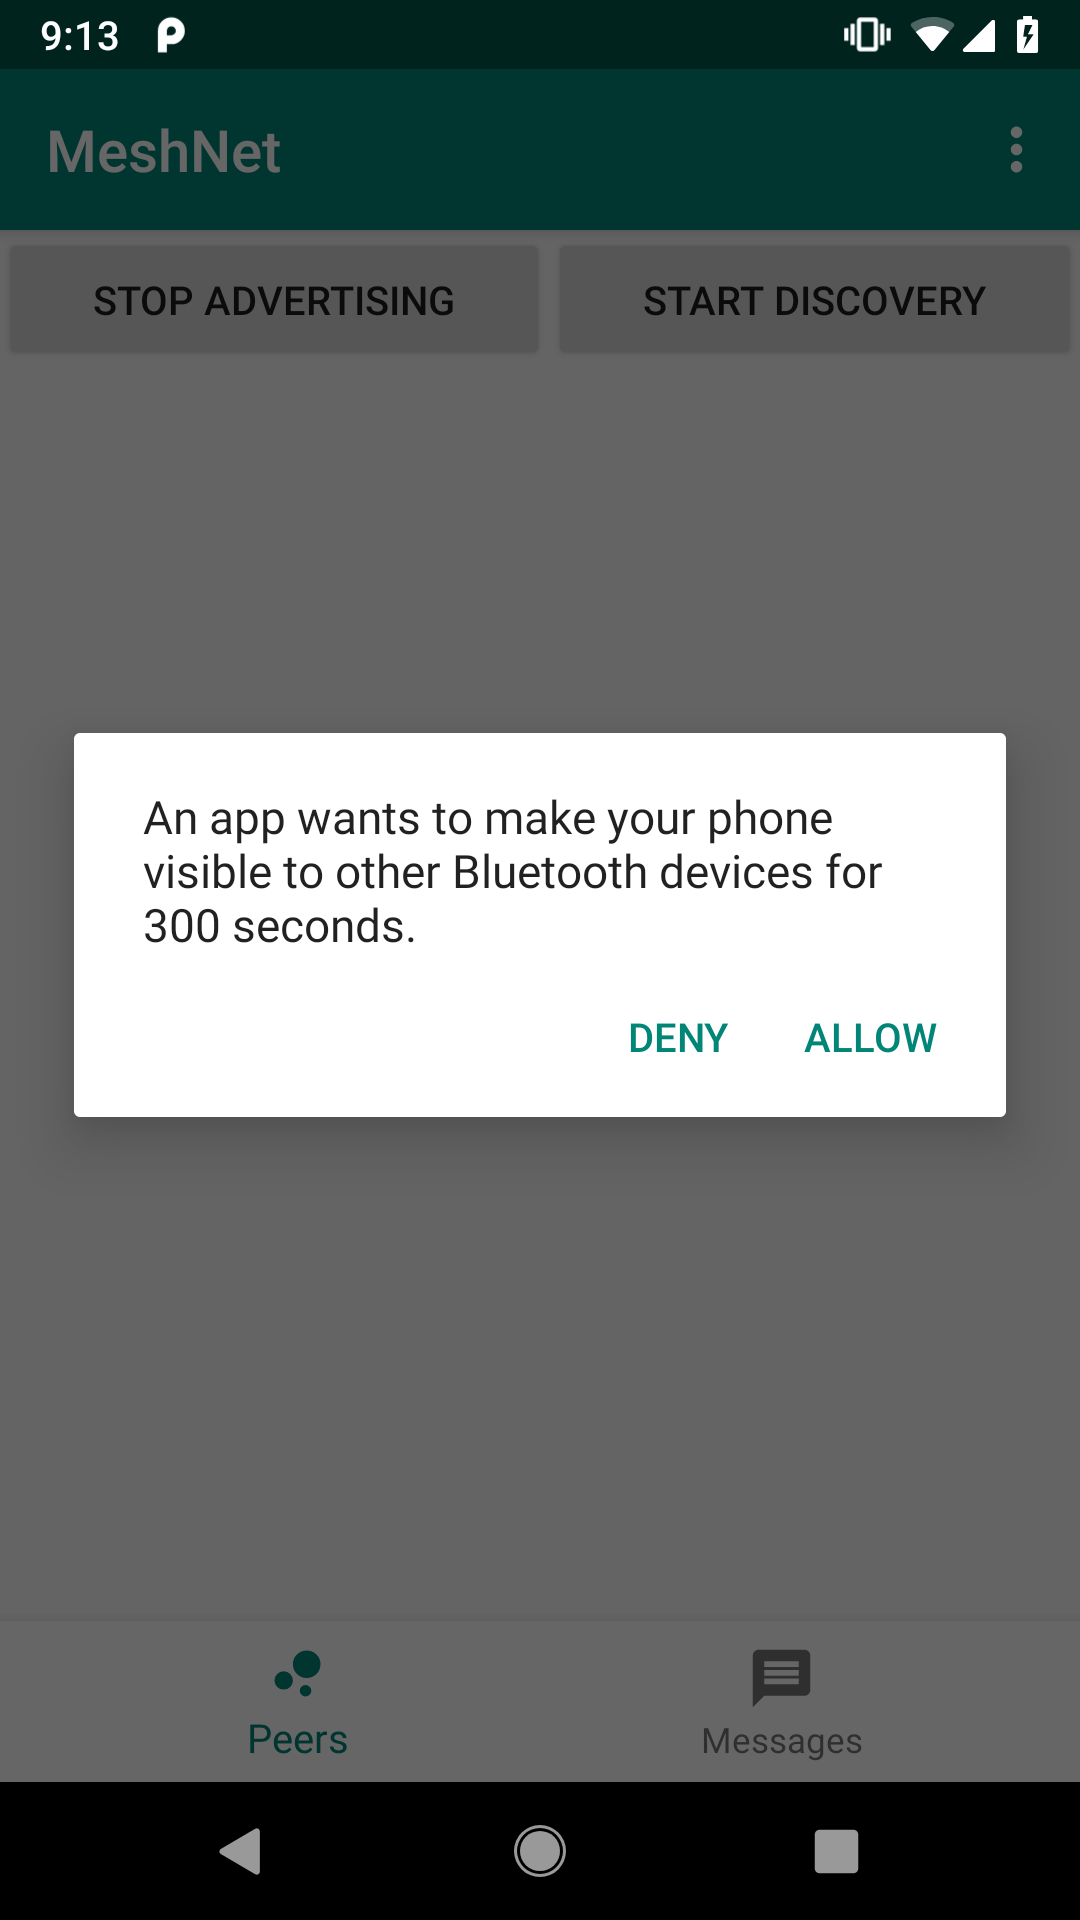
\includegraphics[width=0.32\textwidth]{screens/dialog_bluetooth-discovery}
    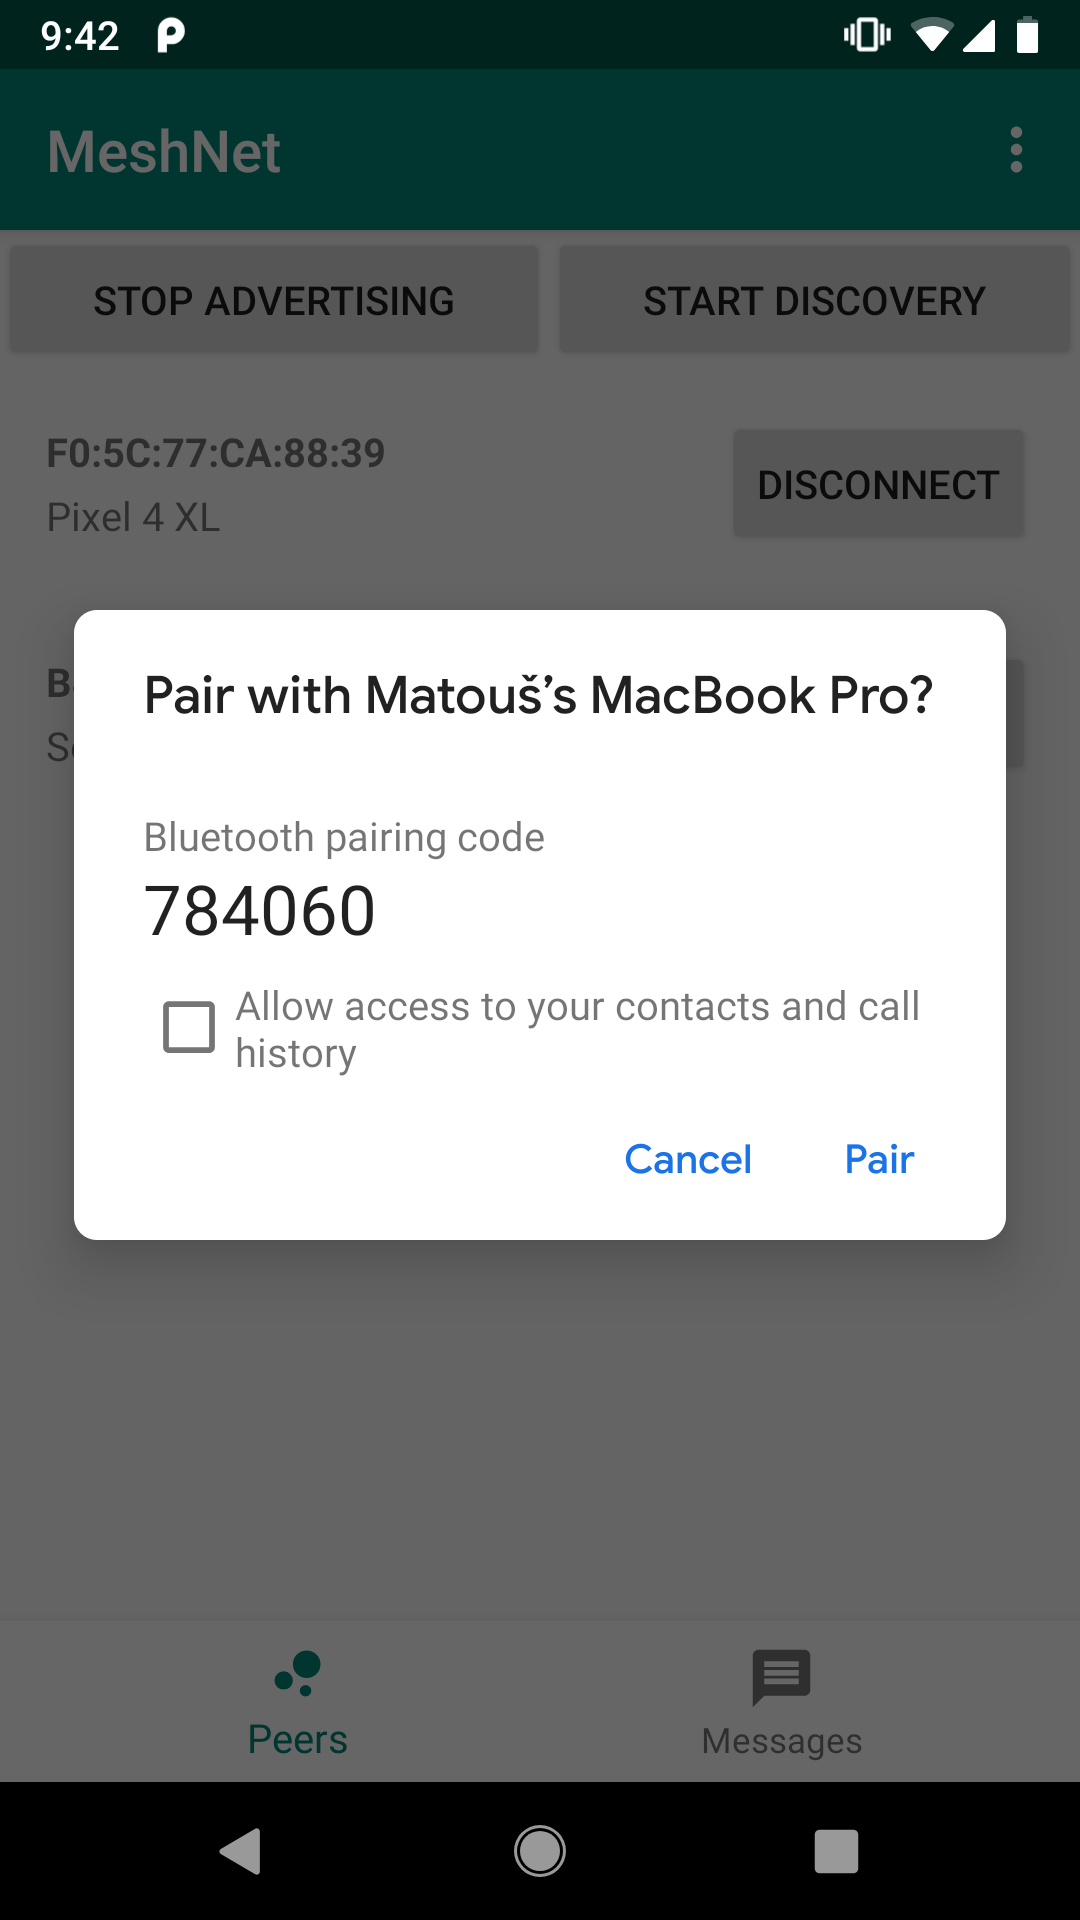
\includegraphics[width=0.32\textwidth]{screens/dialog_bluetooth-pairing}
    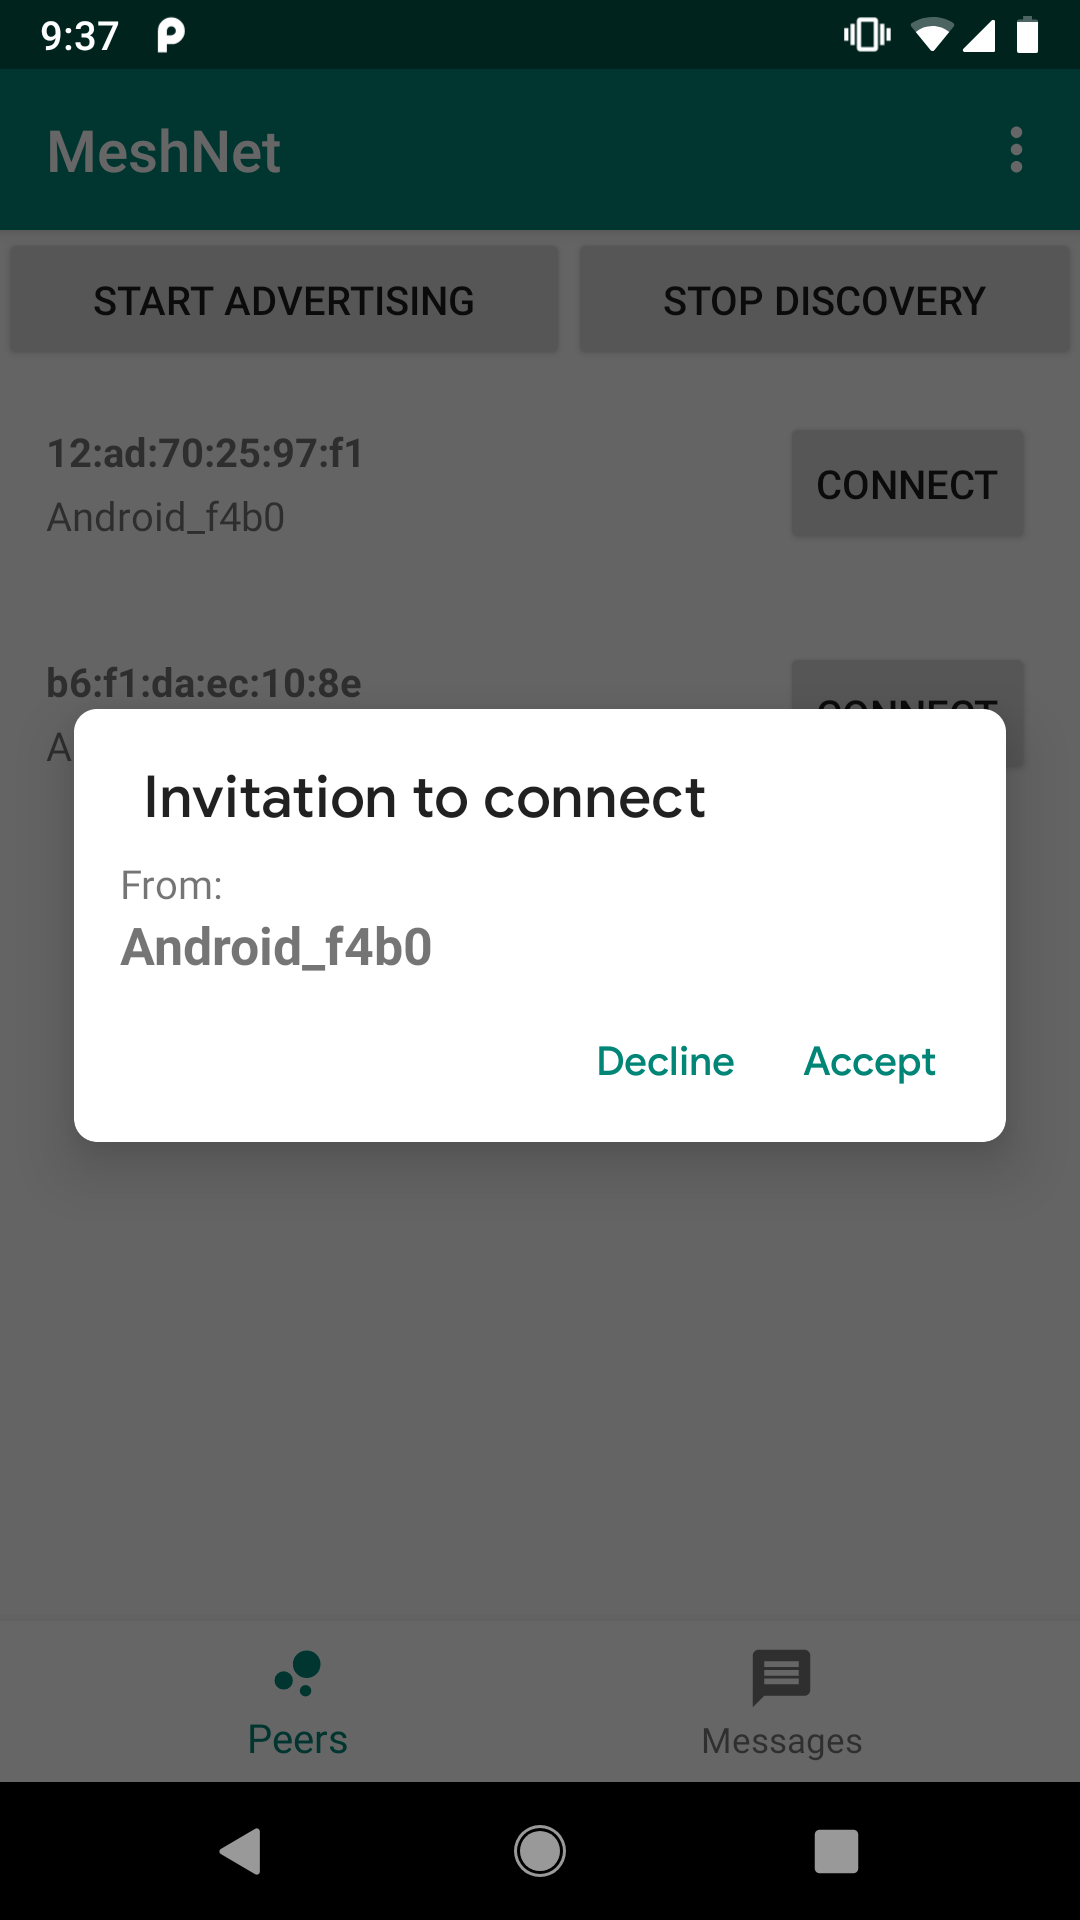
\includegraphics[width=0.32\textwidth]{screens/dialog_wifi-direct}
    \caption{The system UI for enabling Bluetooth discovery, accepting an incoming Bluetooth pairing request, and accepting an incoming Wi-Fi Direct connection on Android 9}
    \label{system_ui}
\end{figure}

% TODO: add screenshots of Bluetooth enable discovery, pairing dialog, WiFi direct dialog

\subsection{Bluetooth}

The oldest and the most battle-tested technology for nearby connectivity is Bluetooth, which has been in development for more then 20 years. The common flow for Bluetooth usage is to first force the user to \textit{pair} (or \textit{bond}) two devices. The device A first needs to manually be set as \textit{discoverable}, usually for a limited time period. The device B then performs a scan to discover nearby devices. The device B can then send a pairing request to the selected device. Then a pairing code is displayed and once both users accept the pairing request, the devices are paired.

Only after that, a secure \textit{Radio frequency communication (RFCOMM)} channel can be established. The pairing process requires user interaction, which degrades the user experience in certain applications when authentication is performed on the application level. While it is possible to establish an \textit{insecure} RFCOMM channel if the MAC address of the other device is known, the user of the other device still needs to manually set it to be discoverable.

\subsection{Bluetooth Low Energy}

% TODO: cite specification

\textit{Bluetooth Low Energy (BLE)} \cite{blebook} was introduced in 2010 as part of the Bluetooth 4.0 specification. It is a completely different communication protocol incompatible with the classic Bluetooth. BLE offers considerably decreased power consumption with a similar communication range and slightly lower bandwidth. It was originally intended to support an infrequent low-power communication with wearables, healthcare accessories, or smart home appliances. However, while it is not a primary use case, it could also be potentially used for low-bandwidth peer-to-peer communication between smartphone devices.

It is notable that once an application is granted a Bluetooth permission, it can fully control BLE APIs without any user interaction, which opens up doors for a range of many different applications.

% use cases: mesh networks
% upper physical throughput: 1 Mbps (modulation rate)

\subsection{Wi-Fi Direct}

There have been many attempts to enable direct communication between IEEE 802.11 radio devices. The 802.11 standard defines two operating modes. Next to the traditional \textit{infrastructure} mode, there is an \textit{ad-hoc} mode which allows device-to-device communication. However, the ad-hoc mode is not supported by Android OS, even though it can be enabled on some devices with a root access.

\textit{Wi-Fi Direct} (also known as Wi-Fi Peer-to-Peer) \cite{wifip2p} is a IEEE 802.11 based protocol released by Wi-FI Alliance in 2009 and supported from Android 4.0. With Wi-Fi direct, devices are organized in groups, where one device is the Group Owner (GO) and the rest are Group Members (GM). The roles are not predefined, but are negotiated during the group formation process. Groups are able to support Legacy Clients (LC), which means that even devices without Wi-Fi Direct support can join as group members.

%\subsubsection{Multi-group communication}

%The standard only defines intra-group communication, but it does not restrict a Group Member from participating in multiple groups simultaneously. Moreover, a device can theoretically connect both to Wi-Fi Direct and an infrastructure network by using multiple virtual MAC entities. However, these functionalities are not defined by the standard and thus depend on the implementation.
%\subsubsection{Limitations of Android}
%In Android, the GO always has the same hardcoded IP address (192.168.49.1), while GM are assigned a random address from the same subnet (192.168.49.2-254). As a result, the scenario where the device would act in multiple groups at the same time cannot be directly implemented.

%There are several workarounds proposed in \cite{FunaiTH16}. The first solution is to use \textit{time sharing} to allow a device to act as a gateway between multiple groups. It requires a device to periodically disconnect and reconnect to different groups and effectively act as a relay passing messages between multiple groups.
%Another solution takes advantage of \textit{simultaneous connections} using Wi-Fi Direct and the traditional Wi-Fi. The GO advertises its group using a unique Service Set ID (SSID) that can be used by other clients not supporting the framework to join the group. Experiments have shown that it is possible to create a LC/GM gateway node when communicating using multicast UDP datagram sockets. Due to routing-related issues, this solution does not work with traditional datagram or stream sockets. The authors also propose a more efficient \textit{hybrid} protocol that uses multicast sockets as a control channel that triggers gateway configuration change if needed. However, all solutions rely on undocumented behaviors, which means their reliability can vary across devices or Android OS versions.

\subsection{Wi-Fi Aware}

\textit{Wi-Fi Aware}, also known as \textit{Neighbor Awareness Networking} (NAN) is a recent networking standard introduced by Wi-Fi Alliance. \cite{wifiaware} It works by forming clusters with nearby devices. The discovery process starts when one device (a \textit{publisher}) publishes a discoverable service. Other devices (\textit{subscribers}) who subscribe to the same service will receive a notification once a matching publisher is discovered. After the subscriber discovers a publisher, it can either send a short message or establish a network connection with the device. A device can be both a subscriber and a publisher simultaneously.

%\subsection{Support in Operating Systems}

% Describe support on different versions of Android
% iOS supports MultipeerConnectivity, no direct access to Wi-Fi Direct
% Bluetooth classic not interoperable, Bluetooth Low Energy the only tech suitable for multiplatform communication

\begin{table}
    \centering
    \begin{tabular}{ | l | l | l | l | l | }
      \hline
      \textbf{Technology} & \textbf{Android} & \textbf{iOS} & \textbf{Throughput} & \textbf{Range} \\
      \hline
      Bluetooth & 2.0+ & 5.0+ & 2 Mbps & $\sim$40 m \\
      \hline
      BLE Advertising & 4.3+ & 6.0+ & \multirow{3}{*}{0.3 Mbps} & \multirow{3}{*}{$\sim$100 m} \\
      BLE GATT & 5.0+ & 6.0+ & &  \\
      BLE L2CAP & 10.0+ & 11.0+ & &  \\
      \hline
      Wi-Fi Direct & 4.0+ & N/A & \multirow{2}{*}{250 Mbps} & \multirow{2}{*}{$\sim$200 m} \\
      Wi-Fi Aware & 8.0+ & N/A & & \\
      \hline
    \end{tabular}
    \caption{The comparison of properties of the most common wireless communication technologies and their support in smarphone operating systems
    }
    \label{wirelesstech_table}
  \end{table}




% technologies available on smartphones:
% - Bluetooth, BLE, WiFi Direct, WiFi Aware
% infrastructureless communication

% Bluetooth Classic
% - requires the device to be discoverable - user interaction
% - no interoperability between iOS and Android
% Bluetooth Low Energy
% - energy efficient, does not require pairing, but lower bandwidth
% - API on Android very low level, error-prone to use
% - role simultaneity – master and slave at the same time

%\section{Goals and Considerations}

\chapter{Protocol Design}

In this chapter, we design a protocol facilitating peer to peer communication between any devices. We start by describing common problems in P2P networks such as identity, peer discovery, data transport, and NAT traversal. For each of the problems, we discuss the solution used by our protocol. In the end, we introduce the architecture of the whole system and describe the interaction between all individual building blocks.

%In this thesis, we will attempt to port the existing IPv8 protocol into Kotlin\footnote{https://kotlinlang.org}, a modern statically-typed language that can be compiled to JVM or native code. This will allow us to run the stack both on desktop and mobile devices without any significant overhead. We will also analyze some weak points of the existing implementation and extend the protocol where needed to be more usable by mobile clients.

It is important to note that in this thesis, we extend an existing IPv8 protocol~\cite{ipv8}. It is desirable that our protocol is backwards compatible with the original py-ipv8 implementation, so that we can connect and communicate with the existing peers in the network and use the services implemented by the existing infrastructure. For that reason, a lot of design decisions that have been previously made had to be accepted as such, even in cases where a different approach would probably be taken in case we designed the protocol from scratch.

\section{Identity and Keys}

In the Internet Protocol, each computer gets assigned an address which is subsequently used for packet routing. The most common version of the protocol, IPv4, uses a 32-byte address space which is not enough to uniquely identify all devices on the planet.
To deal with address exhaustion, internet providers were forced to deploy \textit{Network Address Translation (NAT)} which allows a single address to be shared across multiple devices. With the rise of portable computers and smartphones, using IPv4 addresses on the application level is problematic as they are dependent on the physical location and should not be considered stable user identifiers. \textit{Mobile IP} \cite{mobileip} is one of the proposals that allows devices to move between networks while maintaining their IP addresses, but its wide adoption is unlikely due to the architectural complexity.

Our goal is therefore to define custom peer identities on the protocol level and abstract IP addresses away from the applications. We also want to be able to sign messages to provide authenticity, and optionally encrypt them so they are readable only by the intended recipients. Both issues can be solved by public key cryptography. We will use elliptic-curve cryptography based on the on \textit{Curve25519}, which has been a de facto industry standard for past few years due to its security properties and absence of restricting patents.

Prior to joining the network, each peer needs to generate a \textit{private key} represented by 32 bytes. It can be used for signing messages to prove their authenticity, or for decrypting encrypted messages. The private key can be in turn used to derive a \textit{public key} by multiplying the generator point of the curve by the private key. This operation is known to be irreversible, so it is computationally infeasible to obtain the private key from the public key. The public key can be shared with other peers and is used to verify that the message has been indeed created by the one who claims to be its sender. Furthermore, it can also be used for encrypting messages that will only be readable by the recipient. Finally, we calculate the hash of the public key to derive the \textit{peer ID}. The peer ID can be used to visualize the identity in the application UI as it is shorter than the public key, but the protocol usually operates with public keys directly. This simple process is shown in Figure \ref{keys}.

\begin{figure}[h!]
    \centering
    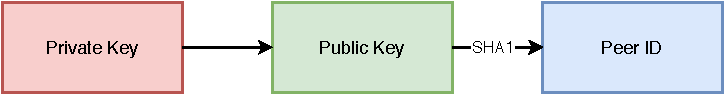
\includegraphics[width=0.8\textwidth]{diagrams/keys}
    \caption{Public key generation process}
    \label{keys}
\end{figure}

\section{Peer Discovery}

Peer discovery is the process of finding other peers in the network we should connect to. It is an essential mechanism in P2P systems as it allows new nodes to join the network.

\subsection{Bootstrap Server}

Probably the most common approach is using one or more bootstrapping servers that acts as trackers. The bootstrap server maintains a list of peers in the network and maintains the list of online peers with regular keep-alive checks. This is the only central component in our system. Ideally, it should be used only for finiding the first few nodes, and after that, the peer discovery would continue using these nodes, without contacting the boostrap server again.

\subsection{Multicast DNS}

When multiple peers are connected to the same local area network and they want to communicate with each other, there should be no need to contact an external server. We could utilize UDP multicast packets to notify other peers in the network who are in the same multicast group. This is the basic principle of the \textit{Local Peer Discovery} protocol used by BitTorrent. Another option would be to use \textit{multicast DNS} (mDNS) mechanism in conjunction with \textit{DNS Service Discovery} (DNS-SD), which is a zero-configuration protocol using packet formats of a DNS system. It allows us to discover local peers providing the given service and connect to them.

\subsection{Bluetooth Advertising}

When peers are in proximity but not connected to the same network, they can still discover each other with some nearby connectivity technologies, such as Wi-Fi Direct, Wi-Fi Aware, or Bluetooth. We have selected Bluetooth Low Energy as it is the most energy efficient and most widely supported technology in today's smartphones. A peer that has Bluetooth turned on is actively broadcasting their identity over advertising packets that can be discovered by other devices. The complete mechanism for nearby communication will be described more in detail in later sections. % TODO: ref

% Distributed hash tables
% Local network broadcast
% Exchanging peer lists with existing peers
% Centralized trackers
% List of bootstrap nodes


\section{Transport Layer}

The transport layer is responsible for transferring data between peers. There are two transport layer protocols implemented in the IP suite: \textit{Transmission Control Protocol (TCP)}, and \textit{User Datagram Protocol (UDP)}.

\subsection{Reliable vs. Unreliable Transport}

TCP provides \textit{connection-oriented}, \textit{reliable} streams. That means that the connection needs to be established before any communication happens. This is done by means of a two-way handshake. Once the connection is established, messages can be exchanged. The messages until they are acknowledged, so the communication is reliable. The sliding window is used for congestion control, so multiple messages can be on the fly at the same time, ensuring efficient usage of the available bandwidth.

On the other hand, UDP is a simple \textit{connectionless} protocol without any delivery guarantees. UDP packets called \textit{datagrams} and its behavior can be described as \textit{fire-and-forget}, as the sender generally does not have any information about packet delivery. It is primarly intended for use in real-time applications where packet loss is acceptable. UDP can also be used for building higher-level transport protocols such as \textit{uTP} or \textit{QUIC}.

Many commonly used protocols such as HTTP take advantage of the reliable transport provided by TCP. However, in P2P setting, UDP is usually favored thanks to its simplicity and absence of a handshake, which makes NAT traveral easier. ICE has been originally defined only for UDP. Though extensions for TCP have been proposed, they rely on a specific NAT behavior to work and have significantly lower success rate than over UDP. For these reasons, we will also choose to use UDP.

\subsection{UDP Socket Multiplexing}



\subsection{Authentication and Encryption}

\subsection{Binary File Transfer over UDP}


%\subsection{NAT Traversal}

%\section{NAT Detection}

\section{NAT Traversal with Peer Introductions}
\label{peer-introductions}

One of the traditional NAT traversal methods called \textit{UDP hole punching} allows to establish UDP connectivity between two peers when both of them are hidden behind a NAT. It is based on the concept that both peers fire a UDP packet targeted at each other at the same time. This first packet creates a mapping entry in the sender's NAT and allows subsequent incoming packets to be delivered. This process can also be seen as opening a \textit{hole} in the firewall, which explains the term \textit{hole punching}.

IPv8 implements a decentralized variant of UDP hole punching mechanism integrated with the peer discovery process, which has been previously described in \cite{nat_wild} and \cite{dispersy}. The complete peer discovery protocol consists of 4 messages and it is visualized in Figure \ref{nat-puncturing}.

After reviewing the py-ipv8 implementation, it has been discovered that it only works reliably when all nodes are behind different NATs. This is because of the fact that the tracker only stores WAN addresses which are then used for peer introductions, and peers always use their WAN address for communication. When multiple nodes are located behind the same NAT, they can still commnicate in case their NAT supports hairpinning, but this is not always the case. There is no mechanism to discover other peers on the same LAN without using a tracker, and there is no way to use LAN addresses for communication. We will fix this flaw by reusing some additional fields which are already present in the IPv8 packet format probably for legacy reasons, but are not currently used. Thanks to that, the updated protocol is still backwards compatible and can be used to connect to peers using older versions of the protocol. The updated protocol works as follows:

\begin{enumerate}
    \item When Alice wants to connect to a new peer in a specific community, it can send an \textit{introduction request} to a tracker, or any other peer present in the community. The introduction request should contain the community ID representing the ID of the community in which Alice wants to find a new peer, and her LAN and WAN address.
    \item We assume Alice sends an introduciton request to Bob. Bob selects a random peer (Charlie) from the requested community, and sends a \textit{puncture request} to him. The puncture request contains the WAN address of Alice.
    \item At the same time, Bob sends an \textit{introduction response} back to Alice. The introducion response contains LAN and WAN address of Charlie.
    \item As soon as Charlie receives a puncture request, he should send out a packet to the WAN address of Alice. That will create a mapping in his NAT, so Alice would be able to contact him.
    \item Alice then keeps sending introduction requests to Charlie's WAN address for a specified interval. After Charlie sends out a puncture packet, the next introduction request should reach him. She can also try to contact him over LAN if they reside in the same subnet.
    \item Charlie should respond to the introduction request with an introduction response, in which he include another peer for introduction. Upon receiving an introduction request or response, the receiver should add the sender to their verified peer list.
\end{enumerate}

\begin{figure}[h!]
    \centering
    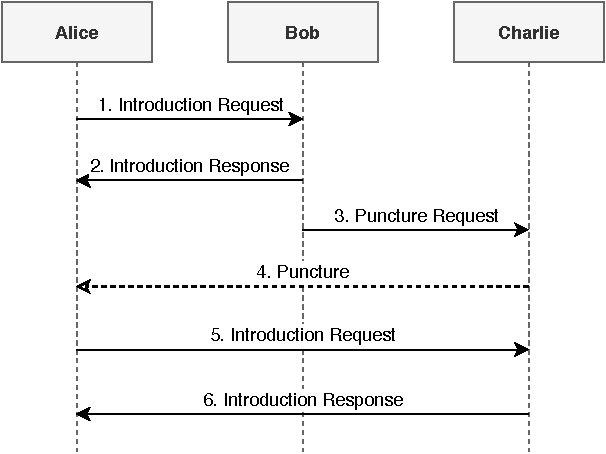
\includegraphics[width=0.8\textwidth]{diagrams/nat-puncturing}
    \caption{Peer discovery mechanism with NAT traversal}
    \label{nat-puncturing}
\end{figure}


\section{Symmetric NAT Traversal}

Our method provided in the previous section allows us to traverse around NATs that perform endpoint-independent mapping. However, as previously discussed in Section \ref{nat-classification}, peers behind NAT with address-dependent mapping would only be able to connect to public peers that do not require NAT traversal. This poses a major threat to our goal of global connectivity.


\subsection{Topological Assumptions}

Inspired by the previously discussed symmetric NAT traversal methods, we have extended our peer introduction protocol to work with some additional NAT behaviors that we encountered during our experimental evaluation of CGN deployments. For the further discussions, we consider three different cases with respect to NAT topology between two different peers A and B:

\subsubsection{Case 1: One peer behind a symmetric NAT}

\begin{enumerate}
    \item Peer A is behind a NAT with endpoint-independent mapping.
    \item Peer B is behind a NAT with endpoint-independent IP address mapping, but an arbitrary port mapping behavior.
    \item Peer B can estimate a session limit implemented by their NAT. By default, the algorithm first assumes there is no limit. In case the first traversal attempt fails, then it falls back to the default limit of 1.000 sessions with a 30-second timeout. This limit has been empirically shown to be successful in all scenarios considered in our experiments. However, the peer should have an option to tweak this parameter if they believe their NAT implements more permissive or restricted behavior.
\end{enumerate}

\subsubsection{Case 2: Both peers behind symmetric NATs without a session limit}
\begin{enumerate}
    \item Both peers are behind a NAT with endpoint-independent IP address mapping, but an arbitrary port mapping behavior.
    \item There is no session limit implemented by any of the NATs.
\end{enumerate}

\subsubsection{Case 3: Both peers behind symmetric NATs with a session limit}
\begin{enumerate}
    \item Both peers are behind a NAT with endpoint-independent IP address mapping, but an arbitrary port mapping behavior.
    \item There is a session limit implemented by one or both of the NATs.
\end{enumerate}

In this case, we need to send packets at the frequency restricted by the session limit. However, as port mappings can frequently change on both sides due to a binding timeout, there is no guarantee when both peers will find find the port mapping. We can keep trying opening ports at random, hoping both peers will meet eventually.
%The statistical model shown in Figure ? shows the probability that the connection will be established based on port discovery process duration.
It is questionable whether it makes sense to support this case, as the effort of establishing the connection might not meet the benefits. It would make sense for long-lived connections that are kept alive for a long period. However, we expect mobile connections to be mostly temporary, so this case has not been implemented while it is theoretically feasible.

Even in the extreme case when the NAT assigns ports completely at random, our NAT traversal mechanism should still work.

The problem is that when a peer A is connecting to peer B behind a symmetric NAT, the peer A does not have a way to find out the public port of peer B.

\subsection{NAT Type Detection}

We would like to have a fully automated NAT traversal. For that, we need a mechanism to decide whether to perform a simple UDP hole punching, or there is a need for an extended multiple UDP hole punching method. We try to detect the NAT type based on its behavioral properties. We keep a log of triples consisting of our LAN address, our WAN address, and peer address. When we detect our LAN address has been mapped to multiple WAN addresses as reported by different remote peers, we can conclude we are located behind a symmetric NAT. Otherwise, we report our NAT type as \textit{unknown}, as it is not necessary to know the exact NAT type for the purposes of UDP hole punching.

\subsection{Extended Peer Introduction Protocol}

\begin{figure}[h!]
    \centering
    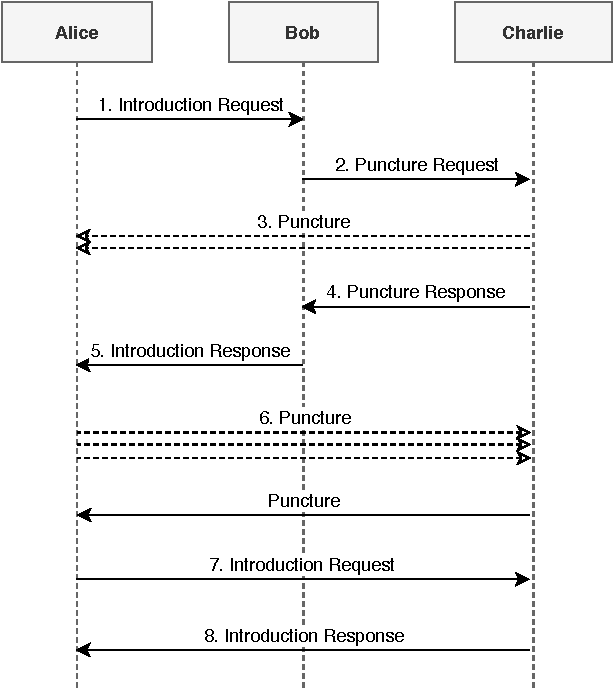
\includegraphics[width=0.8\textwidth]{diagrams/symmetric-nat-puncturing}
    \caption{The flow diagram of the symmetric NAT traversal protocol}
\end{figure}


%\section{Relay Protocol with Bandwidth Accounting}

\section{Security Considerations}

\subsection{Sybil Attack}
\subsection{Eclipse Attack}
\subsection{Distributed Denial of Service}
\subsection{WAN Address Forgery}

\clearpage

\section{P2P Communication with Nearby Devices}

\subsection{Introduction to Bluetooth Low Energy}

In this section, we introduce the most important Bluetooth Low Energy concepts defined in the Bluetooth specification \cite{bluetooth51spec}. This background knowledge is fundamental for understanding the subsequent sections. In principle, there are two methods that BLE devices can use for communication: using connectionless \textit{broadcasting}, or by establishing \textit{connections}.

\subsubsection{Broadcasting}

BLE advertising packets are used to broadcast data to multiple peers at the same time. Other devices can run a \textit{scanning} procedure to read advertisement packets. Each advertisement packet can carry 31-byte payload to describe its capabilities and or any other custom information. Optionally, the scanning device can request a \textit{scan response} from the advertiser, in which the advertiser can send an additional 31-byte payload. That means 62 bytes in total can be transmitted using the broadcasting mechanism. It is important to note that this is unidirectional data transfer and the broadcaster has no way to specify who can receive those packets, or receive any acknowledgements.

\subsubsection{Connections}

An advertising packet can be marked as \textit{connectable}. In that case, if data have to be transferred bidirectionally or more than 62 bytes are required, a connection between two devices can be established.

Devices in BLE can act in two roles: \textit{centrals} and \textit{peripherals}. A central repatedly scans for advertising packets broadcasted by peripherals and when needed, it initiates a connection. A peripheral then periodically broadcasts advertising packets and accepts incoming connections. There are no restrictions on connection limits imposed by the specification. Since Bluetooth 4.1, a single device can act both as a central and peripheral at the same time, and it can also be connected to multiple centrals/peripherals.

\subsubsection{Address Types}

The BLE protocol stack differentiates between two types of addresses. The \textit{public address} is a standard IEEE-assigned MAC address that uniquely identifies the hardware device. Since all BLE packets include a device address, it would be possible to track device movement by adversial scanners. BLE addresses this issue by using a \textit{random address} for any communication. This address is generated using the combination of a device \textit{identity resolving key} and a random number, and it can be changed often, even during the lifetime of a connection.

\subsection{BLE Protocol Stack}

The BLE standard is composed of several protocols which form the BLE stack visualized in Figure \ref{ble_stack}. The stack is split in two parts: a \textit{controller} and a \textit{host}. The controller is usually implemented in hardware, while the host is a part of the operating system. Both parts communicate over the \textit{Host Controller Interface (HCI)}. Even though the applications usually communicate only with the highest layers, it is worth to understand how all layers of the stack fit together. In this section, we describe the responsibilities and mechanics of each protocol.

\begin{figure}
    \centering
    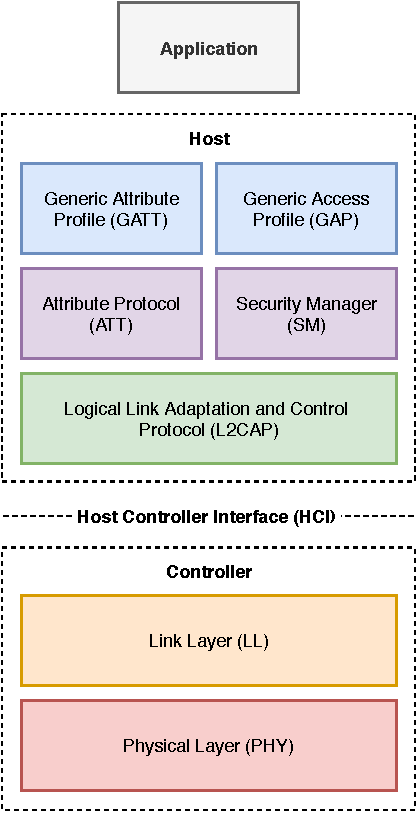
\includegraphics[width=0.40\textwidth]{diagrams/ble-stack}
    \caption{Bluetooth Low Energy Protocol Stack \cite{blebook}}
    \label{ble_stack}
\end{figure}

\subsubsection{Logical Link Control and Adaptation Protocol (L2CAP)}

On the lowest layer in the host, L2CAP is responsible for multiplexing and splitting data from higher-level protocols (ATT and GAP) into 27-byte data packets. These are then forwarded to the Link Layer and transmitted over the Physical Layer implemented in the Bluetooth radio. Starting with Bluetooth 4.1, the applications can communicate over L2CAP directly. User-defines channels allow for higher-throughput data transfer without the additional complexity added by ATT.

% \subsubsection{Security Manager (SM)}

%\subsubsection{Generic Access Profile (GAP)}
% // TODO

\subsubsection{Attribute Protocol (ATT)}
ATT is a client-server protocol for reading and writing attributes. It is strict about sequential operation. If a request is pending, no further requests should be sent until the response is received, otherwise they are discarded. Attributes are stored under attribute handles defined by UUIDs. Various operations are defined by the protocol. Apart from the standard configuraiton, read and write, queued write is supporte to write data longer than a single packet. If a client wants to be notified about handle changes, it can subscribe to handle value notifications or indications. Both allow the server to notify the clients whenever a value changes, but in case of indication, the client should respond with ack packet to confirm it has received the indication.

\subsubsection{Generic Attribute Profile (GATT)}

The Generic Attribute Profile defines how to exchange data between devices. It uses ATT as a transport protocol. The data are organized hierarchically in \textit{services} which contain groups of related data called \textit{characteristics}, which can be further specified using \textit{descriptors}.

GATT is a client–server protocol and it follows the same principles as ATT. A client sends requests to the server and receives responses or server-initiated updates. The server is responsible for storing data written by the client and responding to read requests. It is important to mention that the client and server roles in GATT are independent of the roles defined by GAP. Both a peripheral and a central can take the role of a client or a server, or even both at the same time.

%\subsection{Using Bluetooth Low Energy for P2P Communication}

%\subsection{Bluetooth Device Address}

\subsection{BLE Communication Architecture}

As mentioned earlier, the primary purpose of BLE was to enable exchange of information with peripheral devices. However, as it is currently the most universal way for nearby communication on mobile devices that does not require any user interaction, it is potentially suitable for any type of communication. Since Android 5.0, it is possible to create a custom GATT server which allows two Android devices to communicate with each other over BLE. We now proceed to designing a system architecture for P2P communication using BLE. The overall high-level architecture of data flow is shown in Figure \ref{ble_architecture}.

\begin{figure}
    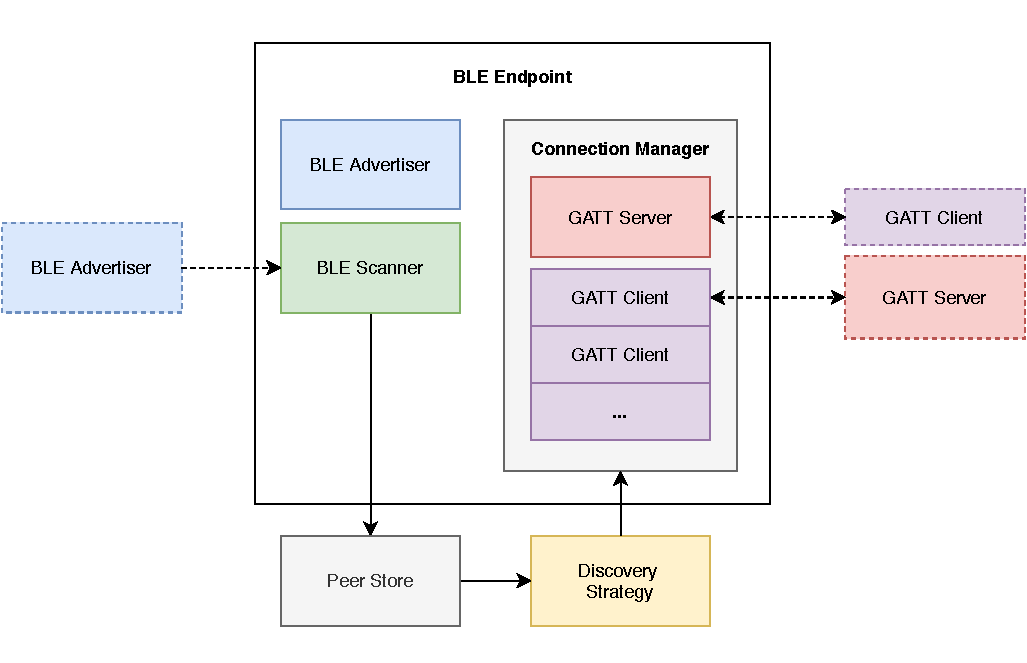
\includegraphics[width=\textwidth]{diagrams/ipv8-ble-architecture}
    \caption{Bluetooth Low Energy Communication Architecture}
    \label{ble_architecture}
\end{figure}

The BLE module should be composed of several submodules with clearly separated responsibilities. The communication begins by the device A broadcasting connectable advertising packets using \textbf{BLE Advertiser}. The advertising packet contains:

\begin{itemize}
    \item a \textit{service UUID} which identifies our application,
    \item a \textit{transmission power level} in dB which can be used by the receiver to calculate a path loss and estimate the distance between devices, and
    \item a \textit{peer ID} which identifies the broadcasting device.
\end{itemize}

The device B then scans for advertising packets using a \textbf{BLE Scanner}. It should filter packets by service UUID to receive only packets relevant to our application. The BLE scan is a power-intensive operation, so it should be performed only when the user actually wants to connect to a new device. It could be done e.g. only when the application is in the foreground. In case we are designing a long-running service that should run in the background, a scan should be run periodically. We should have an option to specify a scan window duration and an interval between individual scans.

Once the scanner receives an advertising packet, it creates a \textit{peer candidate} which consists of a peer ID, a Bluetooth device address which can be used to initiate a connection, a transmission power level in dB, and a received signal strength (RSSI) in dBm. It stores the peer candidate into the \textbf{Peer Store}.

The \textbf{Discovery Strategy} is responsible for selecting which peer we should connect to. The strategy should be application-specific and can e.g. prefer to connect to devices with the largest RSSI value, or to connect only to known peers based on their peer ID. Once the strategy selects a peer it wants to contact, it is sent to the \textbf{Connection Manager}.

The connection manager contains all GATT-related communication logic. Each device has exactly one GATT server and an arbitrary number of GATT client instances, one for each device it is connected to. The GATT server implements a single GATT service containing two characteristics which are shown in Figure \ref{gatt_server}. The \textbf{Public Key} characteristic has a \textit{readable} permission and simply contains a public key of the peer. It is used to determine the identity of the device when initializing the connection and can be used for authentication and encryption in the further communication. The \textbf{Writer} characteristic with a \textit{writable} permission is then used for sending data from the client to the server. As we want to support bidirectional communication, every two devices need to have a pair of client–server and server–client connections. This can be implemented in a way that every time a GATT server receives an incoming connection, the connection manager initiates an outgoing connection to the GATT server of the connecting device. Only after both links are established, the connection is considered ready.

\begin{figure}
    \centering
    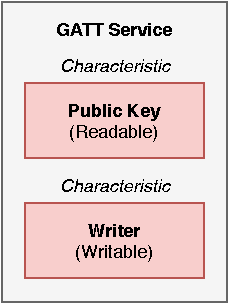
\includegraphics[width=0.25\textwidth]{diagrams/ipv8-gatt}
    \caption{Our GATT Server Architecture}
    \label{gatt_server}
\end{figure}

% GATT - service, characteristic, descriptor
% Service IPv8
% Characteristics
% - Member ID, permission read
% - Writer, permission write
% Handshake
% - 1. Read Member ID
% - 2. Wait for other peer to read our Member ID
% - 3. Send data to peer via its Writer

% Future Work:
% - L2CAP connection oriented channels (Android 10+)

% https://medium.com/@martijn.van.welie/making-android-ble-work-part-3-117d3a8aee23
% https://stefanbossbaly.com/2018/08/06/ble-in-android
% https://blog.classycode.com/a-short-story-about-android-ble-connection-timeouts-and-gatt-internal-errors-fa89e3f6a456
% https://punchthrough.com/android-ble-development-tips

\chapter{Protocol Implementation}

In this section, we describe the system architecture and implementation of the P2P communication library. One of our main goals is to create an implementation that would be compatible with the majority of mobile devices. The most commonly used operating systems are Android and iOS, where Android uses the Android Runtime, with primary programming language being Java or Kotlin. iOS runs ARM native code compiled from Objective-C or Swift. Both platforms support running native code and allow the use of bridges to access system APIs. We are primarily interested in supporting Android, but extension for iOS support should be possible in the future.

Regarding the programming language choice, many options have been considered. In general, there are three approaches to mobile development. The first one is to write the core logic in a language that compiles to native code and compile it as library for all possible CPU architectures. \textit{Rust}\footnote{https://www.rust-lang.org/} was considered as a low-level language that compiles to native code. It provides good performance and its compiler is proven to prevent any race conditions in a multi-threaded code. However, it could only be used to develop the core library, and the UI would still need to be written in languages supported by the specific platform SDK.

Another approach is using a multi-platform framework that allows to reuse most of the code including the UI. Probably the most prevalent multi-platform framework today is \textit{React Native}\footnote{https://reactnative.dev/} developed by Facebook. However, it comes with the overhead of running in the JavaScript engine and despite its name, does not really provide a native performance.
%Another alternative is Flutter developed by Google, which uses a custom language \textit{Dart}\footnote{https://flutter.dev/} and a completely custom rendering engine. However, while stable, it is still considered an experimental technology.

The last and the most common approach is to use the languages officialy supported by the platform SDK. \textit{Kotlin}\footnote{https://kotlinlang.org/} is a modern statically typed language that can be compiled into JVM, native code, or JavaScript. It has been officially supported as the official programming language for Android since 2017 \cite{androidkotlin} and has replaced Java as the primary language in 2019. Thanks to its ability to compile to native code using the Kotlin/Native compiler, it can also be compiled for other platforms such as iOS. In the end, We have chosen Kotlin as the language for implementing both the P2P library and eventually the application itself.

% Android vs. iOS, interoperability
% Kotlin, Multiplatform - JVM + Android, but can be compiled to Native for iOS as well
% Android Things – IoT


\section{System Architecture}

The architecture of kotlin-ipv8 is heavily inspired by the architecture of the original py-ipv8 library, with some extensions. %Therefore, this section also serves as the documentation of the existing protocol, which is mostly missing at the moment, and had to be reconstructed by reading the existing codebase.
The basic architectural building blocks are visualized in Figure \ref{ipv8_architecture}.

A \textit{community} is a service implemented by the developer, or provided by the core of the library. Every service using the library should be extending the base \texttt{Community} class which provides convenient methods for serializing and deserializing messages, and reading the list of peers who are present in the community from the \textit{peer store}. It also implements messaging required for peer introduction and NAT puncturing mechanism previously described in Section \ref{peer-introductions}.

Every community can have assigned one or more \textit{dicovery strategies}. A discovery strategy is primarily responsible for actively discovering and connecting to new peers in the network who are present in the same community. The discovery strategy should implement a method \texttt{takeStep} that is called reguarly in a preconfigured step interval and performs the required task.

Finally, an \textit{endpoint} is used to perform the communication. The library supports multiple transports implemented by separate endpoints. To abstract this away from the application developer, the community only communicates with the \textit{endpoint aggregator}. It groups all endpoints and decides to which endpoint the message should be sent. The messages received by the endpoint are then forwarded to the correct community based on the message header.

\begin{figure}
    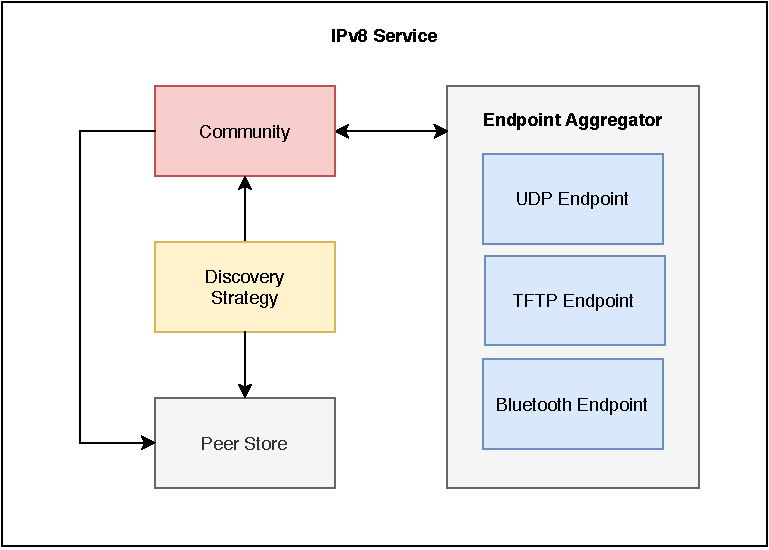
\includegraphics[width=\textwidth]{diagrams/ipv8-architecture}
    \caption{The system architecture of the IPv8 service}
    \label{ipv8_architecture}
\end{figure}

\section{Communities}

\subsection{Community}

Each community has to extend the abstract \texttt{Community} class which implements the \texttt{Overlay} interface. The only field left for the developer to define is \texttt{serviceId}. This can be an arbitrary 20-byte array represented as a hexadecimal string that uniquely identifies the community. The Community class defines several methods that can be used by its subclasses:

\begin{itemize}
    \item \texttt{getPeers(): List<Peer>} – Returns the list of connected peers that are present in this community.
    \item \texttt{serializePacket(messageId: Int, payload: Serializable, sign: Boolean, encrypt: Boolean, recipient: Peer?): ByteArray} – Serializes a payload into a binary packet that can be sent over the transport.
    \item \texttt{send(peer: Peer, data: ByteArray)} – Sends a packet to the target peer.
    \item \texttt{send(address: Address, data: ByteArray)} – Sends a packet to the target IPv4 or Bluetooth address.
\end{itemize}

\subsection{Discovery Community}

\texttt{DiscoveryCommunity} is one of the core communities implemented by the IPv8 core. It tries to keep an active connection with a specified number of peers and keeps track of communities they participate in by sending \textit{similarity requests}. A similarity requests contains a list of communities the sender supports, and expects to receive a \textit{similarity response} back, which will include the list of communities supported by the other side. Furthermore, it implements \textit{ping} and \textit{pong} messages that allow to perform keep-alive checks, measure latency between peers, and handle peer churn by removing churned peers from the peer store. While it is possible to run IPv8 without using this community, it is not recommended. The discovery community is expected to be used with \texttt{PeriodicSimilarity} and \texttt{RandomChurn} strategies.


% \subsubsection{Ping}

% send random int, measure latency

% \subsubsection{Similarity Request}

\section{Discovery Strategies}

\subsection{Random Walk}

\texttt{RandomWalk} is a simple discovery strategy that performs a random walk in the network. On every step, it requests a new peer introduction by sending an introduction request to a random connected peer. At the same time, a random peer from peer candidates (the list of introduced, but not yet contacted peers) is selected, and greeted with an introduction request. If the peer does not respond with the introduction response within a specified timeout (3 seconds by default), it is removed from the peer candidate list.

\subsection{Periodic Similarity}

The \texttt{PeriodicSimilarity} strategy simply sends a similarity request on every step to a random peer in the peer store, and thus ensures the list of communities for every peer is kept up to date. It is only intended to be used for \texttt{DiscoveryCommunity}.

\subsection{Random Churn}

The \texttt{RandomChurn} strategy starts by selecting a list of random peers on every step. Each peer in the list is classified either as \textit{active}, \textit{inactive}, or \textit{churned}. The peer is considered churned if we haven't received a response to a ping in the last 57.5 seconds. In that case, we drop the peer from the peer store. The peer is considered inactive if we haven't received a response in the last 27.5 seconds. In that case, we send a ping to check for liveliness. If the peer is still active, we only send a ping if we haven't send it yet, to calculate the latency. The magic constants for detecting inactive and churned peers have been adopted from the original py-ipv8 implementation, as they have been extensively tested in the wild and are expected to reflect the behavior of the majority of NAT boxes. \cite{nat_wild}

\subsection{Bluetooth Discovery Strategy}

\section{Endpoints}

\subsection{Endpoint Aggregator}

\subsection{UDP Endpoint}

\subsection{TFTP Endpoint}

\subsection{Bluetooth Endpoint}

\section{Bootstrap Server}

The bootstrap server is used by new peers who are interested in joining the network. It is implemented by extending the base community class with a customized behavior. The server accepts and responds to introduction requests regardless on the community id sent in the header, which enures that the bootstrap server can be used for discovering peers in any community. Upon the introduction request, it adds a peer to its peer store, and responds with an introduction response that contains the link IP address of the peer as it was received on the socket, and a random peer from the community from which the request was send. Peer churn is handled by a \texttt{SimpleChurn} strategy that simply removes any peers that have not sent any message in the last 120~seconds.

The bootstrap server can be started with the following command, where a port can be specified in the \texttt{port} Java property:

\begin{minted}{bash}
./gradlew :tracker:run -Dport=8090
\end{minted}

The list of default bootstrap servers that are contacted upon initialization is defined in the \texttt{Community.DEFAULT\_ADDRESSES} field.

\section{Project Structure}

The project consists of two sub-projects that are maintained in two separate repositories: the P2P library called \textit{kotlin-ipv8}\footnote{https://github.com/Tribler/kotlin-ipv8}, and the application built on top of this library. The kotlin-ipv8 library currently supports Android and JVM targets, and the project is composed of the following modules:

\begin{itemize}
    \item \texttt{ipv8} \textit{(JVM library)}: The core of the IPv8 implementation, a pure Kotlin library module.
    \item \texttt{ipv8-android} \textit{(Android library)}: Android-specific dependencies and helper classes for running IPv8 in Android Runtime.
    \item \texttt{demo-android} \textit{(Android app)}: An Android application demonstrating the initialization of the \texttt{ipv8-android} library.
    \item \texttt{ipv8-jvm} \textit{(JVM library)}: JVM-specific dependencies for running IPv8 on JVM.
    \item \texttt{demo-jvm} \textit{(JVM app)}: The CLI app demonstrating the usage of the \texttt{ipv8-jvm} library.
    \item \texttt{tracker} \textit{(JVM app)}: The bootstrap server implementation.
\end{itemize}

The ipv8 module contains the core logic that is shared across JVM and Android platforms. To ensure the stability of the project and make contributions by other developers easier, a development and \textit{continuous integration (CI)} infrastructure has been set up. The tests are written using the test framework \textit{JUnit}\footnote{https://junit.org/} and mocking framework \textit{mockk}\footnote{https://mockk.io/}. The code coverage is calculated and reported using \textit{Java Code Coverage Library (JaCoCo)}. The \textit{ktlint}\footnote{https://ktlint.github.io} linter is used to ensure the consistent code style, and Android Lint to check for common errors related to the usage of Android SDK. All tools are run automatically for every commit and merge request by a \textit{GitHub Actions} workflow. \textit{codecov.io}\footnote{https://codecov.io} is used to report the changes in code coverage for every pull request. The ipv8 module has extensive code coverage of 72\%.

%The Gradle build system is used to specify the build and runtime dependencies.

% JVM vs. Android
% unit tests, TODO: Android tests
% library vs. super app separation

% \section{Maintaining Backward Compatibility}
% continuous improvement while maintaining backward compatibility with 10 year old ipv8 implementation

\iffalse
\section{Library Usage}

In this section, we describe the usage of the kotlin-ipv8 library from the perspective of the application developer. We will show how to create a simple overlay network, and send and handle custom messages. Finally, we will configure and start the IPv8 stack, and load our overlay with a discovery strategy, which will allow us to discover other peers in the community using the bootstrap server.

\subsection{Project Setup}

To include the library in an Android app, the application developer should first include the kotlin-ipv8 repository as a Git submodule. In the future, the library could be deployed to a maven repository. At that point Git submodule would not be needed and the application could depend on a specific version of the library.

The Android application module should depend on the ipv8-android module which includes and exposes APIs of the ipv8 module, and defines some Android-specific dependencies and helper classes. The dependency can be defined by adding the following line to \texttt{build.gradle}:

\begin{minted}{groovy}
implementation project(':ipv8-android')
\end{minted}

\subsection{Creating a Community}

All communities have to extend an abstract \texttt{Community} class, which implements the \texttt{Overlay} interface. The only field left for us to define is \texttt{serviceId}. This can be an arbitrary 20-byte array represented as a hexadecimal string that uniquely identifies the community. We therefore generate a serviceId and define a \texttt{DemoCommunity} class:

\begin{minted}{kotlin}
class DemoCommunity : Community() {
    override val serviceId = "02313685c1912a141279f8248fc8db5899c5df5a"
}
\end{minted}


\subsection{Generating a Private Key}

Every peer in has to generate a key pair which establishes the identity and is used to sign and verify messages. We can generate a private key with \texttt{AndroidCryptoProvider.generateKey()}. The key can then be serialized to a byte array with \texttt{Key.keyToBin()} method, and again deserialized using \texttt{AndroidCryptoProvider.keyFromPrivateBin(ByteArray)}. When the app is launched for the first time, the key should be generated and persisted. The previously generated key should be loaded on subsequent launches.

\subsection{Library Initialization}

We now proceed to initialize IPv8 and load our overlay. While it is possible to instantiate \texttt{IPv8} class directly, on Android it is easier to prepare \texttt{IPv8AndroidFactory} and call \texttt{IPv8Android.init} method to initialize the stack.

First, we define a configuration for our overlay \texttt{OverlayConfiguration} consists of an overlay factory and a list of discovery strategies. We can either define our own factory extending \texttt{Overlay.Factory} if we need to provide custom parameters to the overlay, or use the default implementation. Then, we create a factory for a discovery strategy. We use \texttt{RandomWalk}, a simple strategy discovering peers by performing a random walk in the network.

\begin{minted}{kotlin}
val demoCommunity = OverlayConfiguration(
    Overlay.Factory(DemoCommunity::class.java),
    listOf(RandomWalk.Factory())
)
\end{minted}

Then, we define \texttt{IPv8Configuration}. The only required parameter is a list of overlays we want to load when the service is started. We pass the configuration created in the previous step.

\begin{minted}{kotlin}
val config = IPv8Configuration(overlays = listOf(
    demoCommunity
))
\end{minted}

Finally, we create \texttt{IPv8AndroidFactory}, set the previously created configuration, our private key, and call the \texttt{init} method. This will start an IPv8 instance and create a foreground Android service to allow it to run even when the app is in the background.

\begin{minted}{kotlin}
IPv8Android.Factory(this)
    .setConfiguration(config)
    .setPrivateKey(getPrivateKey())
    .init()
\end{minted}

The init method will return an instance of \texttt{IPv8Android} that can be used to access loaded overlays and communicate with them from the UI code. Alternatively, the IPv8 singleton instance can also be accessed with \texttt{IPv8Android.getInstance()}.


\subsection{Sending and Receiving Messages}

Now that we have multiple peers connected, we can perform some communication. First, we define a custom payload type implementing \texttt{Serializable} and \texttt{Deserializable} interfaces:

\begin{minted}{kotlin}
class MyMessage(val message: String) : Serializable {
    override fun serialize(): ByteArray {
        return message.toByteArray()
    }

    companion object Deserializer : Deserializable<MyMessage> {
        override fun deserialize(
            buffer: ByteArray,
            offset: Int
        ): Pair<MyMessage, Int> {
            return Pair(MyMessage(buffer.toString(Charsets.UTF_8)),
                buffer.size)
        }
    }
}
\end{minted}

Next, we define a function in the DemoCommunity class which will iterate over all peers and send a message to all of them. We also define a message ID that is included as a prefix to the serialized message. The same ID will be used later to register a message handler for this message type.

\begin{minted}{kotlin}
private const val MESSAGE_ID = 1

fun broadcastGreeting() {
    for (peer in getPeers()) {
        val packet = serializePacket(MESSAGE_ID, MyMessage("Hello!"))
        send(peer.address, packet)
    }
}
\end{minted}

Finally, we add a message handler to parse incoming messages and print their sender and content to the log.

\begin{minted}{kotlin}
init {
    messageHandlers[MESSAGE_ID] = ::onMessage
}

private fun onMessage(packet: Packet) {
    val (peer, payload) = packet.getAuthPayload(MyMessage.Deserializer)
    Log.d("DemoCommunity", peer.mid + ": " + payload.message)
}
\end{minted}

\fi


\chapter{Decentralized Super App}

The application follows the concept of a super app, and bundles many mini-applications in a single APK. It is implemented in a separate repository \textit{trustchain-superapp}\footnote{https://github.com/Tribler/trustchain-superapp} and includes kotlin-ipv8 as a Git submodule.

\begin{figure}
    \centering
    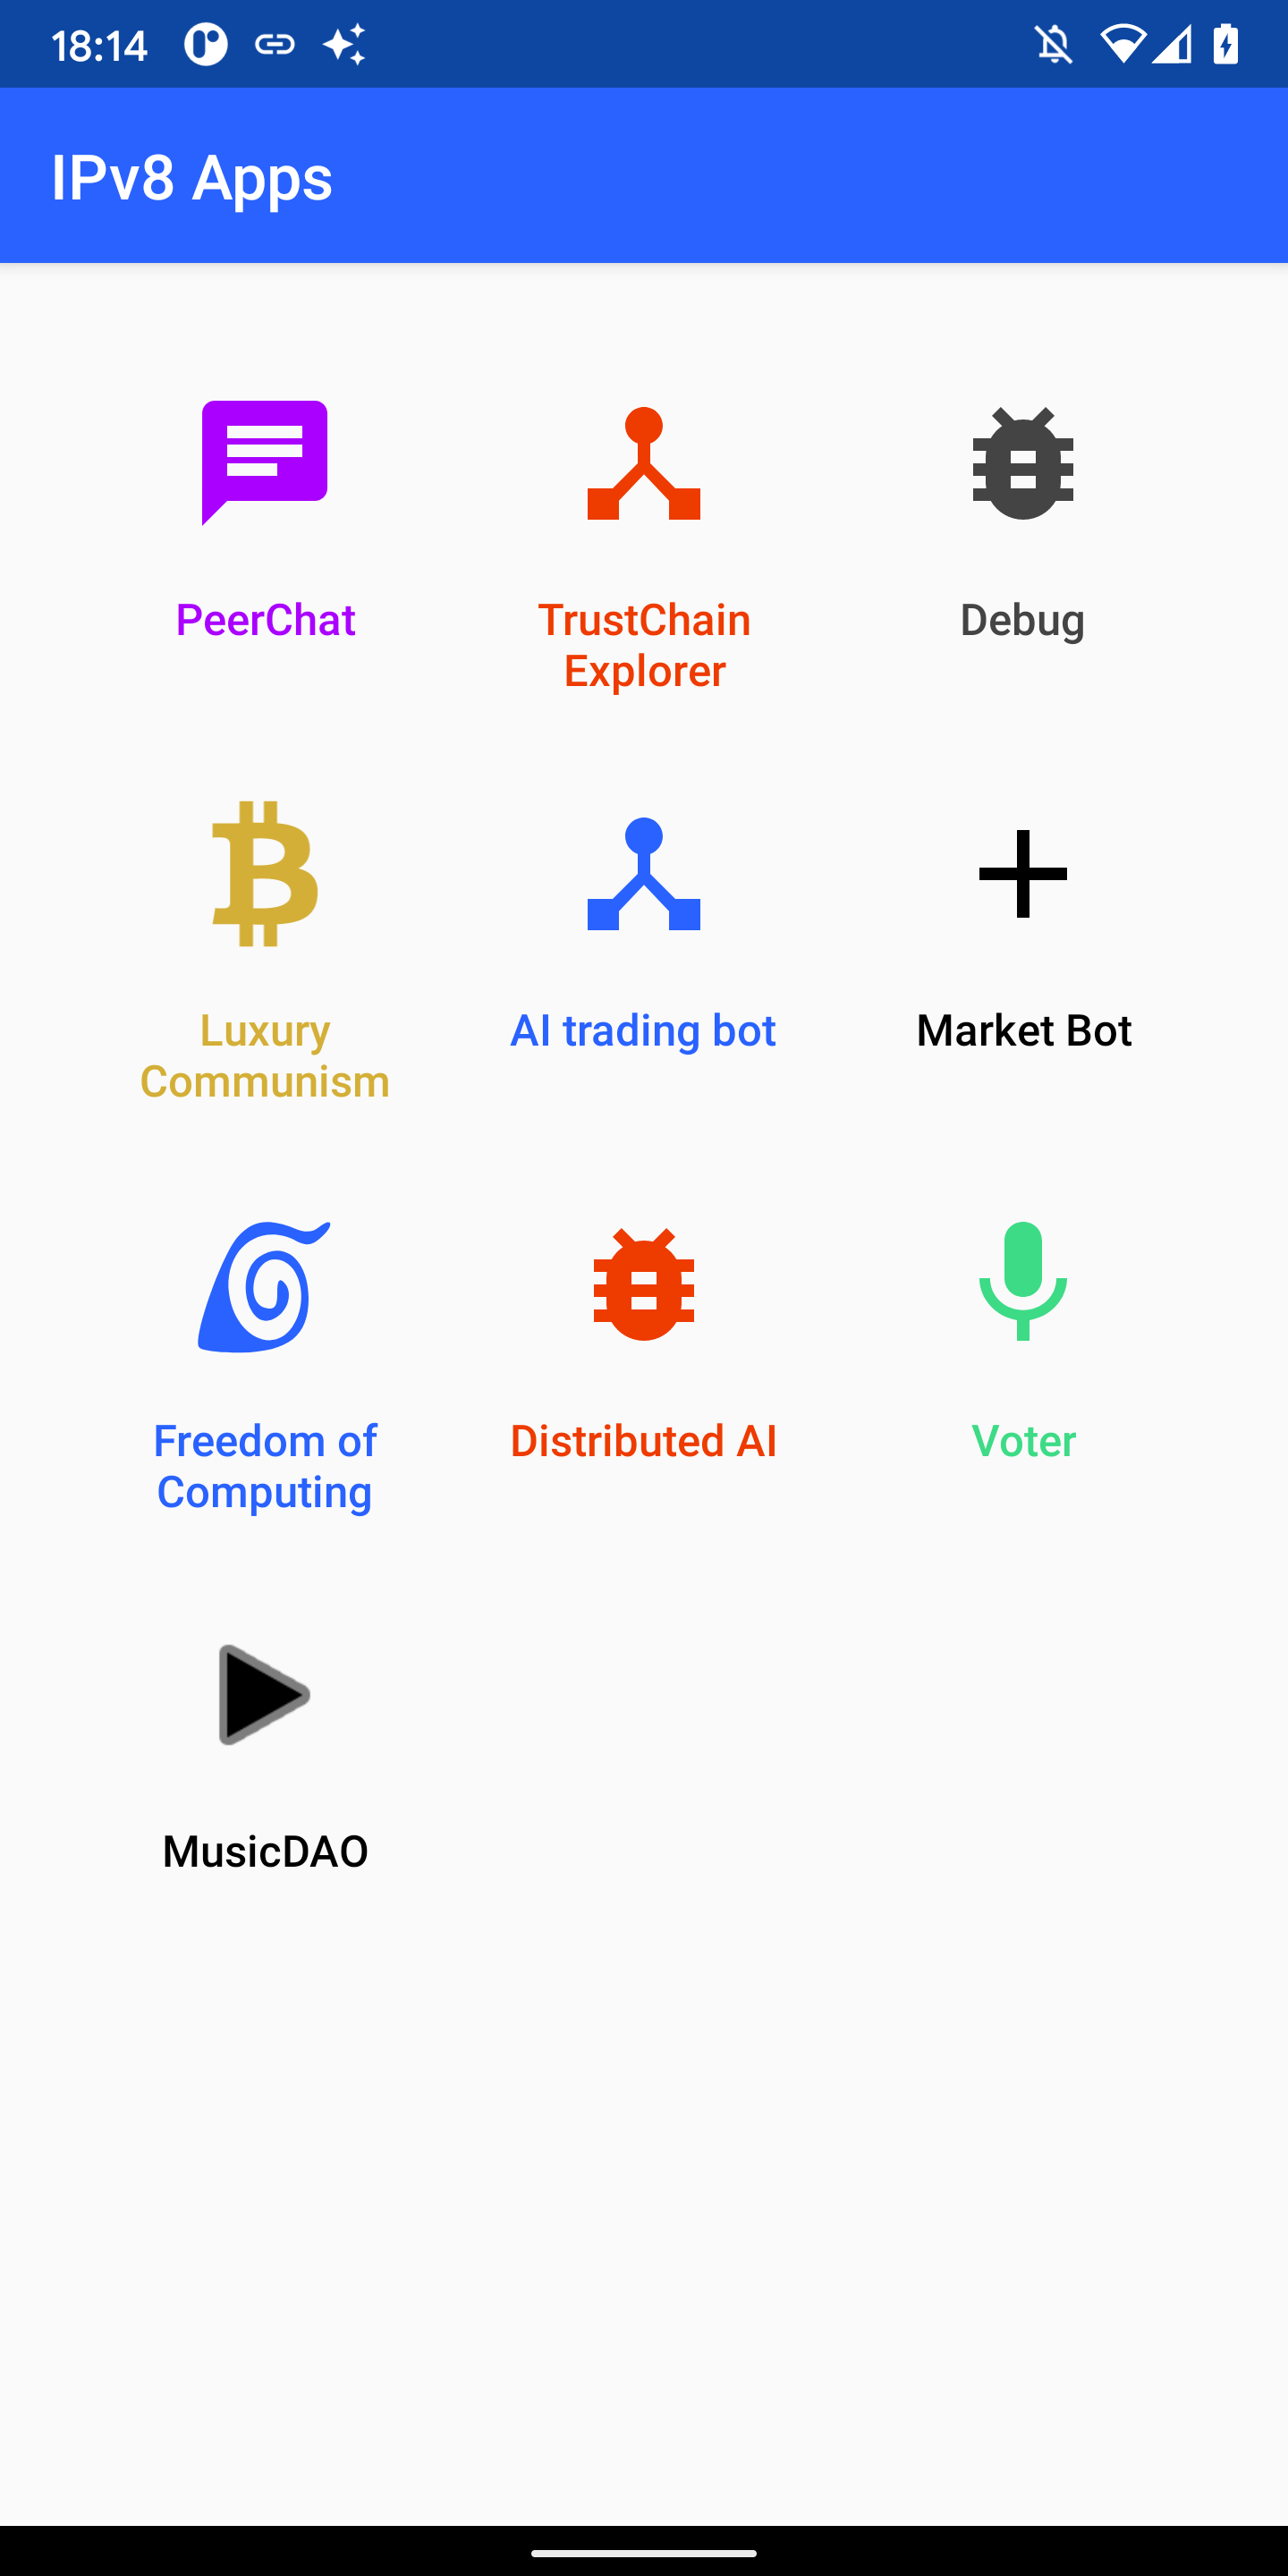
\includegraphics[width=0.32\textwidth]{screens/superapp/superapp}
    \caption{The dashboard of the super app composed of several decentralized mini-apps implemented on top of the kotlin-ipv8 library and TrustChain.}
    \label{manyverse}
\end{figure}

\section{TrustChain: Scalable Distributed Ledger}

\subsection{TrustChain Explorer}

\section{PeerSocial: Decentralized Social Network}

\subsection{Trustworthy Friendship Establishment}

\begin{figure}
    \centering
    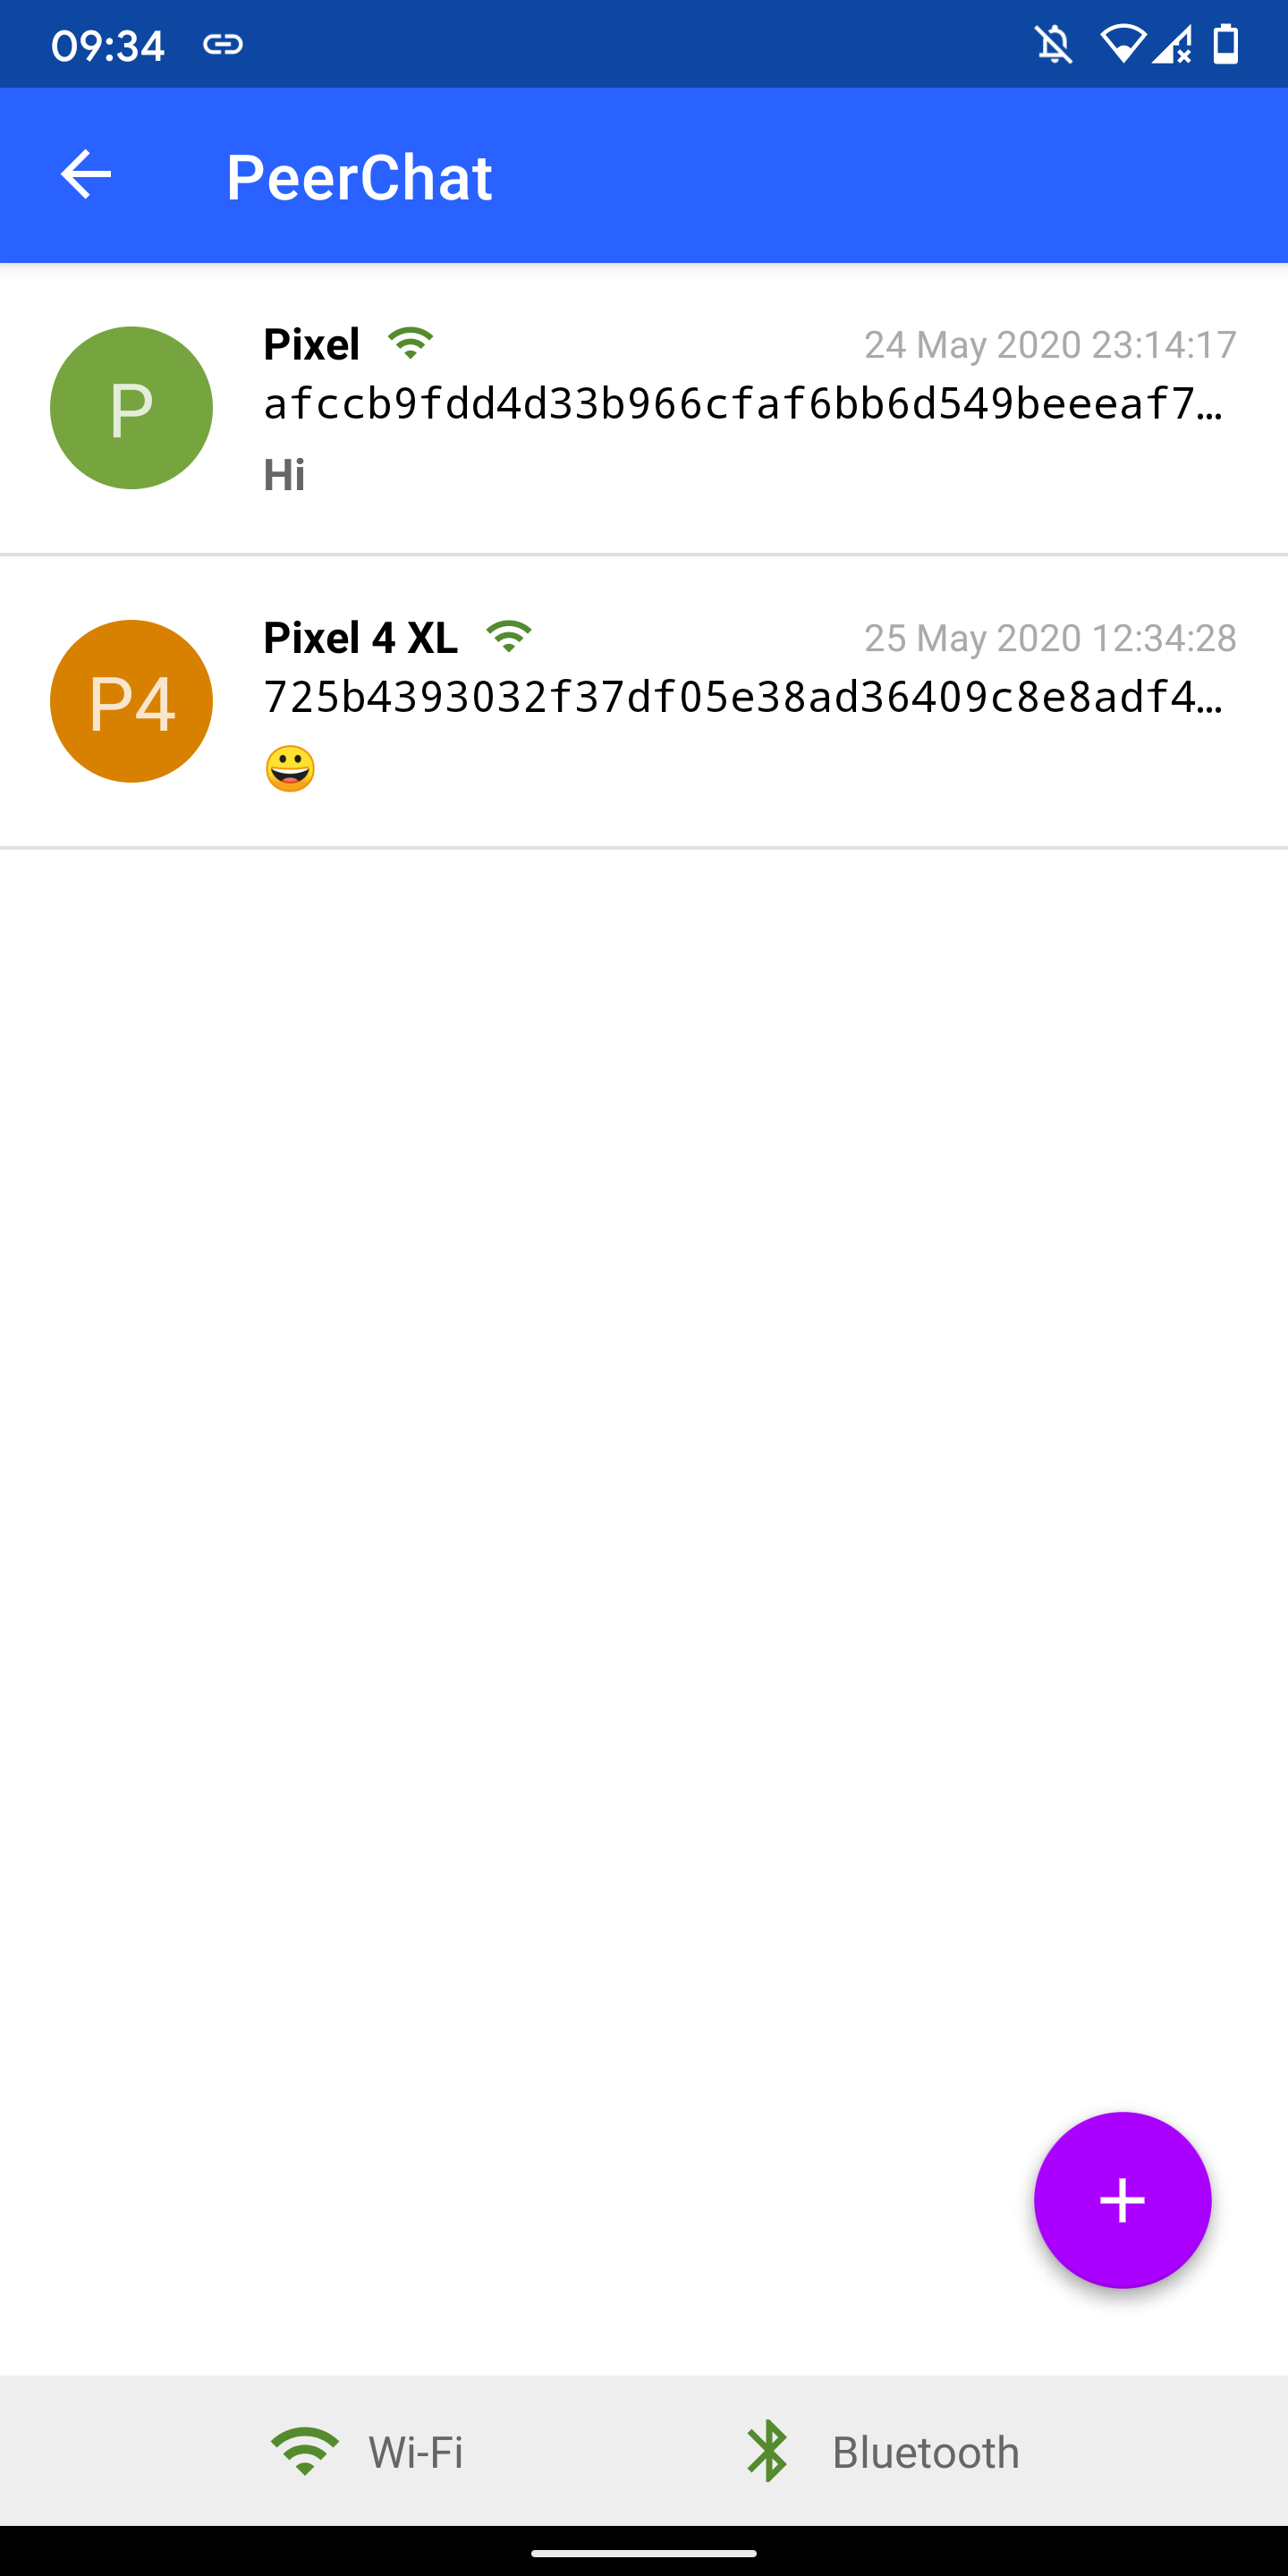
\includegraphics[width=0.32\textwidth]{screens/superapp/contacts}
    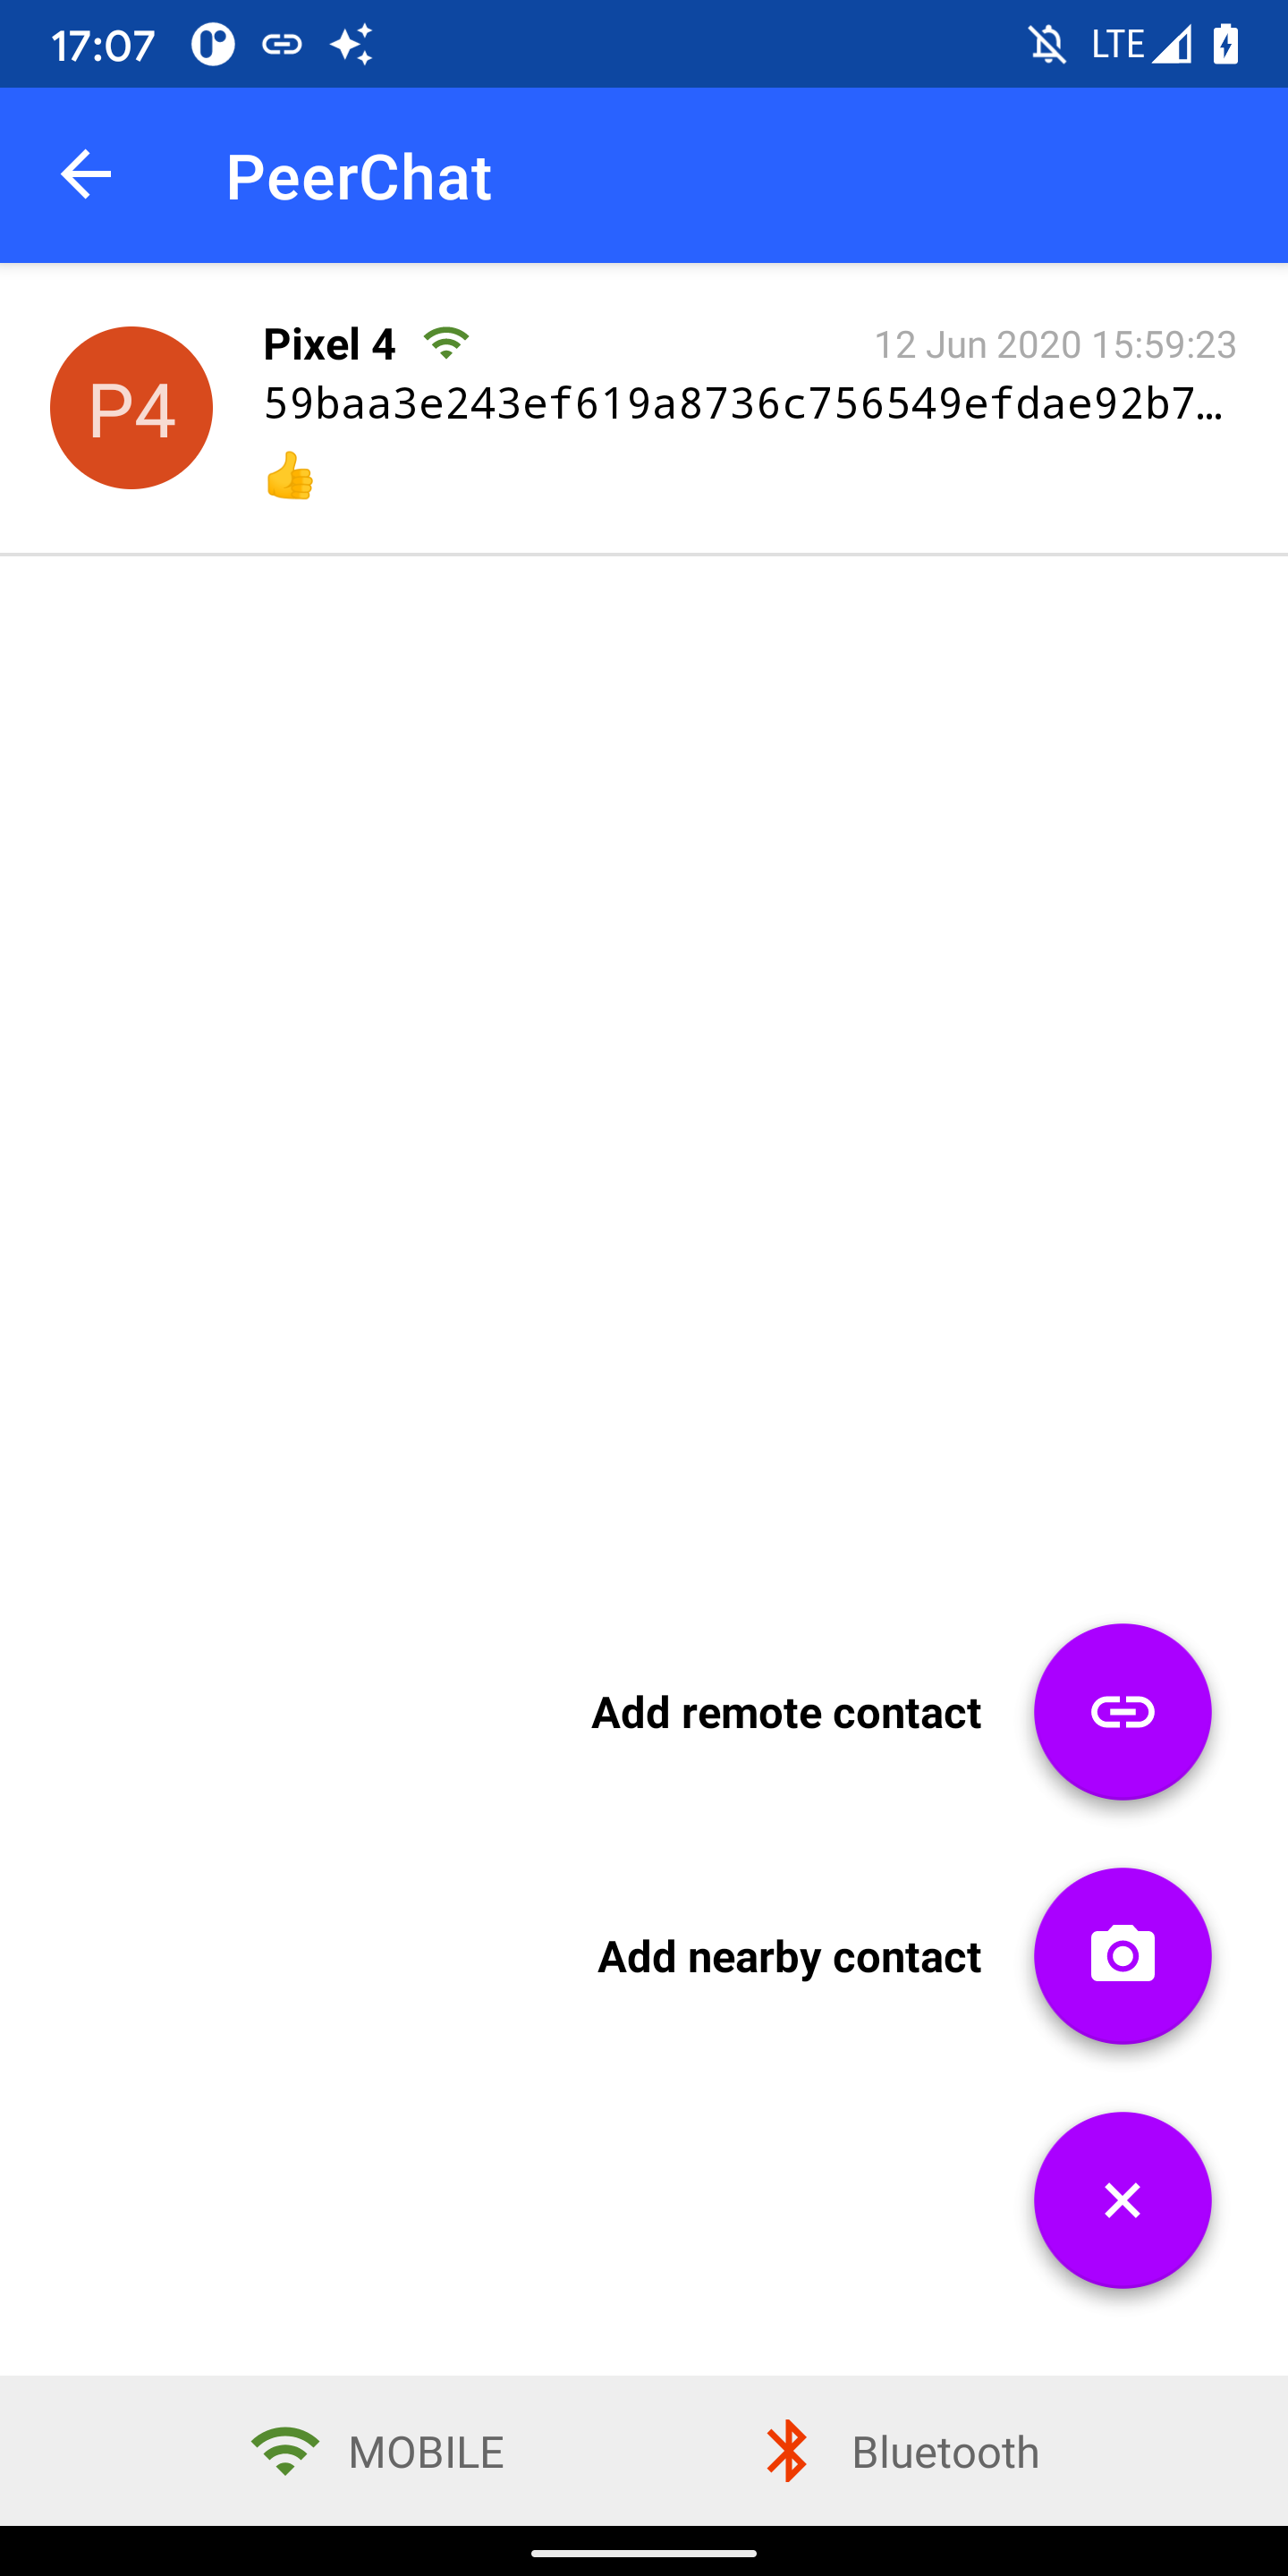
\includegraphics[width=0.32\textwidth]{screens/superapp/contacts_menu}
    \caption{The list of contacts with online indicators, their latest messages with timestamps, and the connectivity status of the local UDP and Bluetooth endpoints.}
    \label{manyverse}
\end{figure}


\begin{figure}
    \centering
    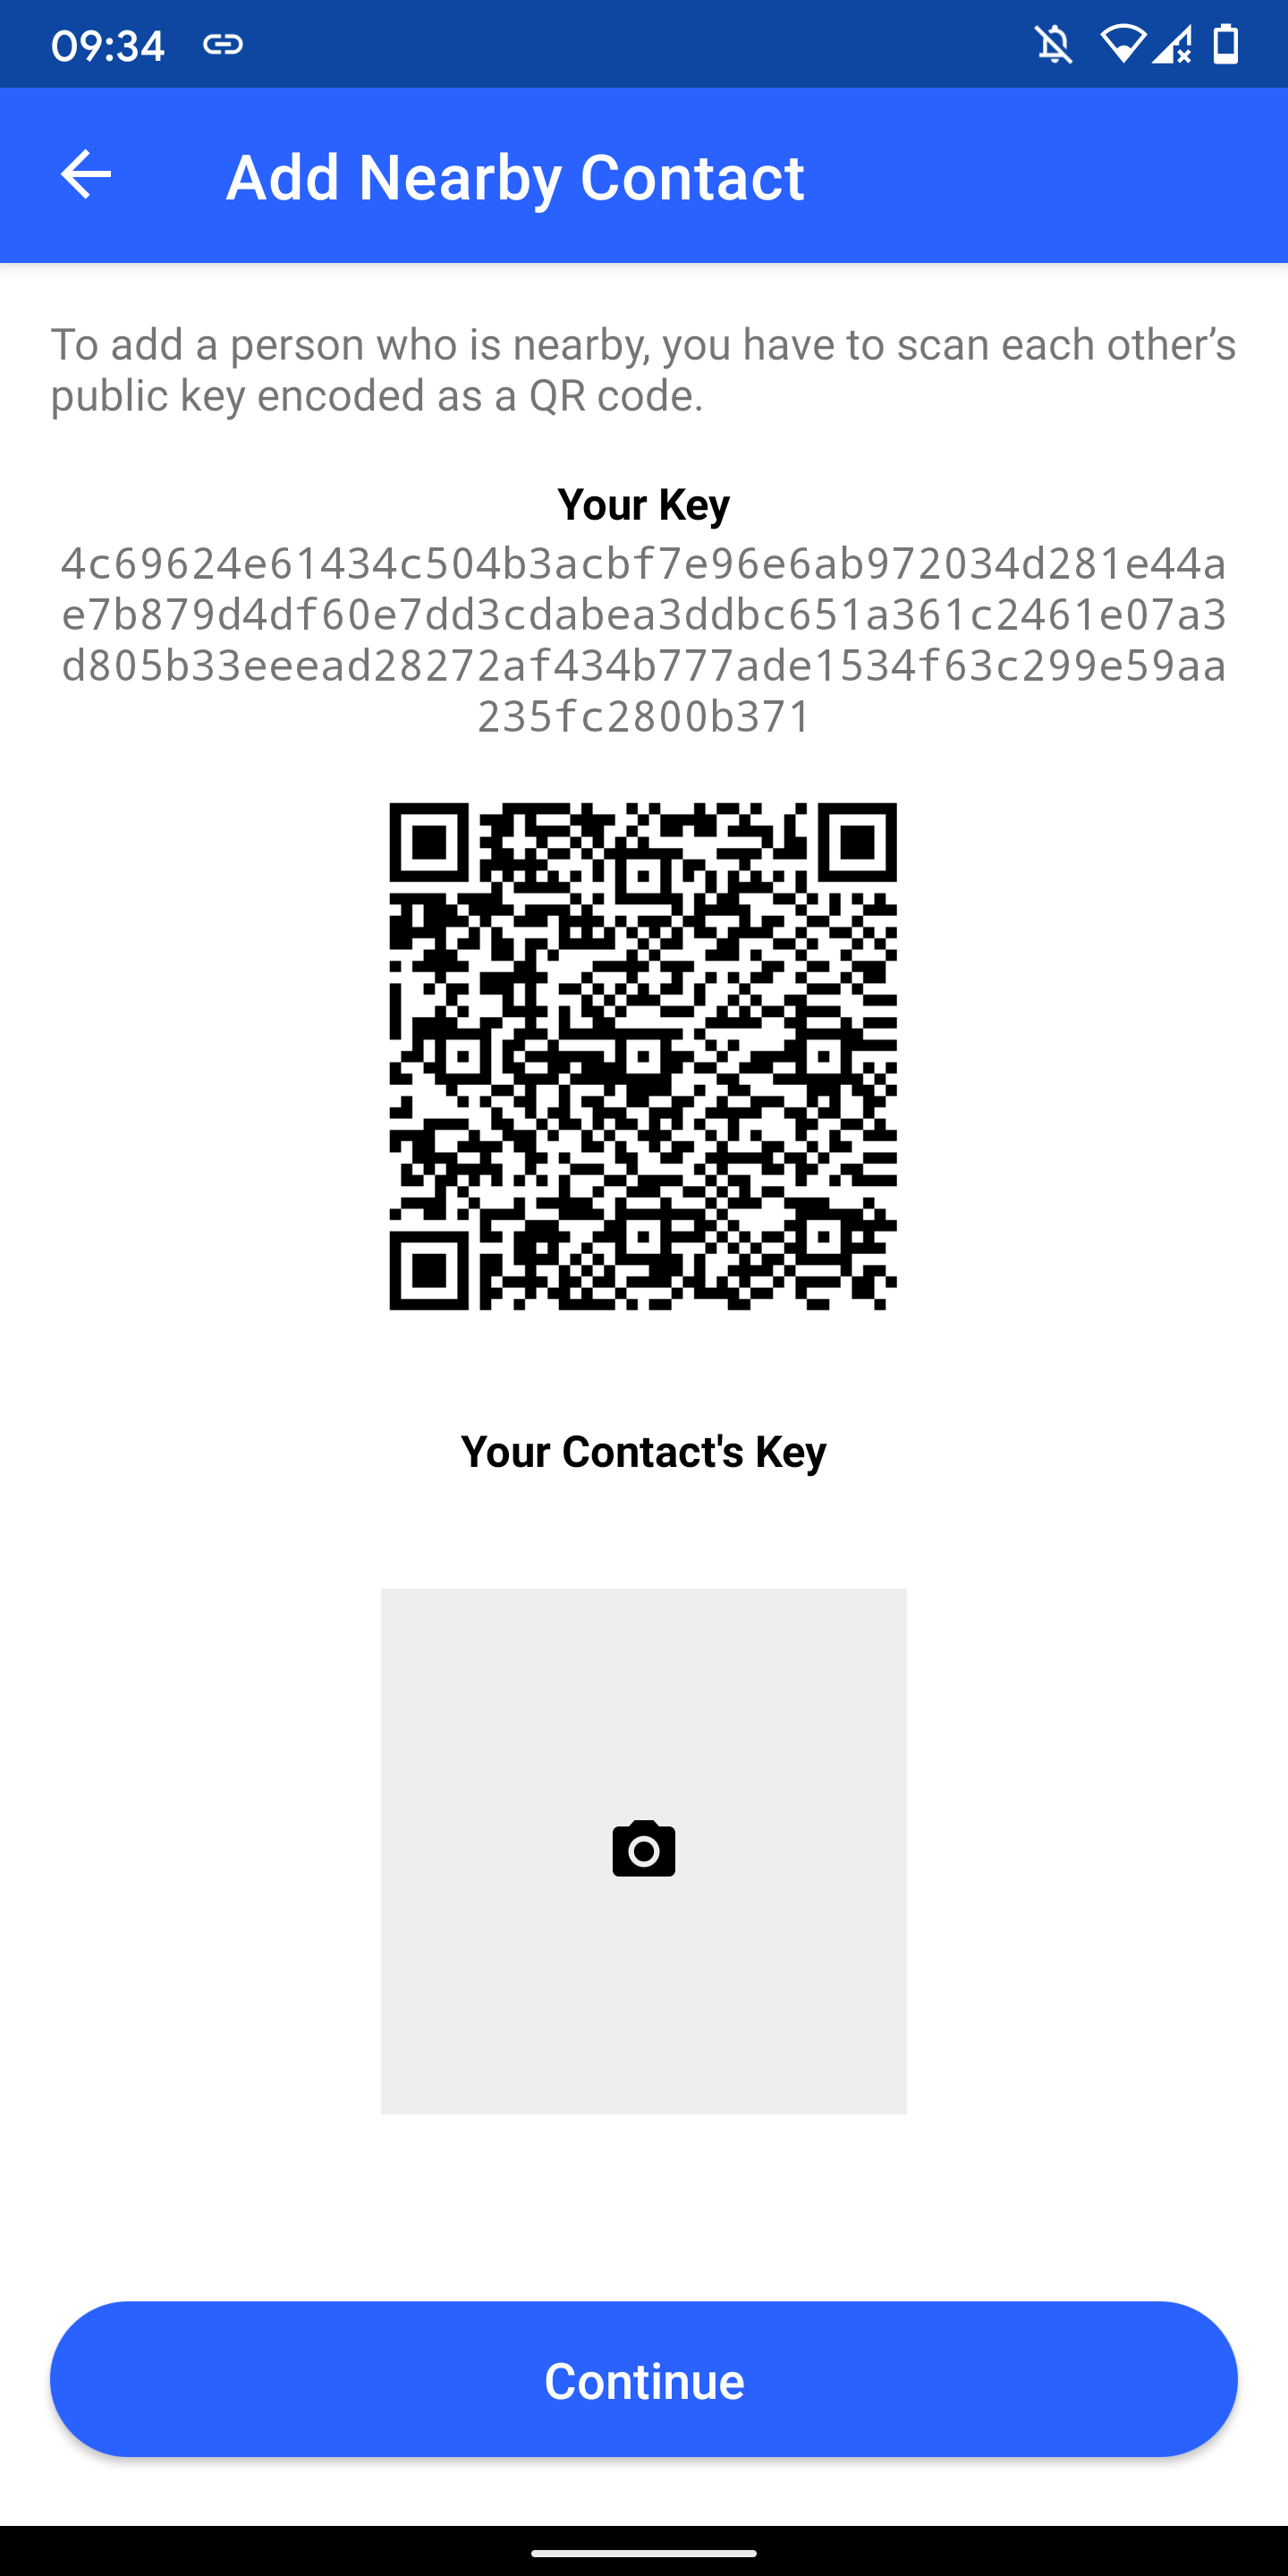
\includegraphics[width=0.32\textwidth]{screens/superapp/add_nearby_contact}
    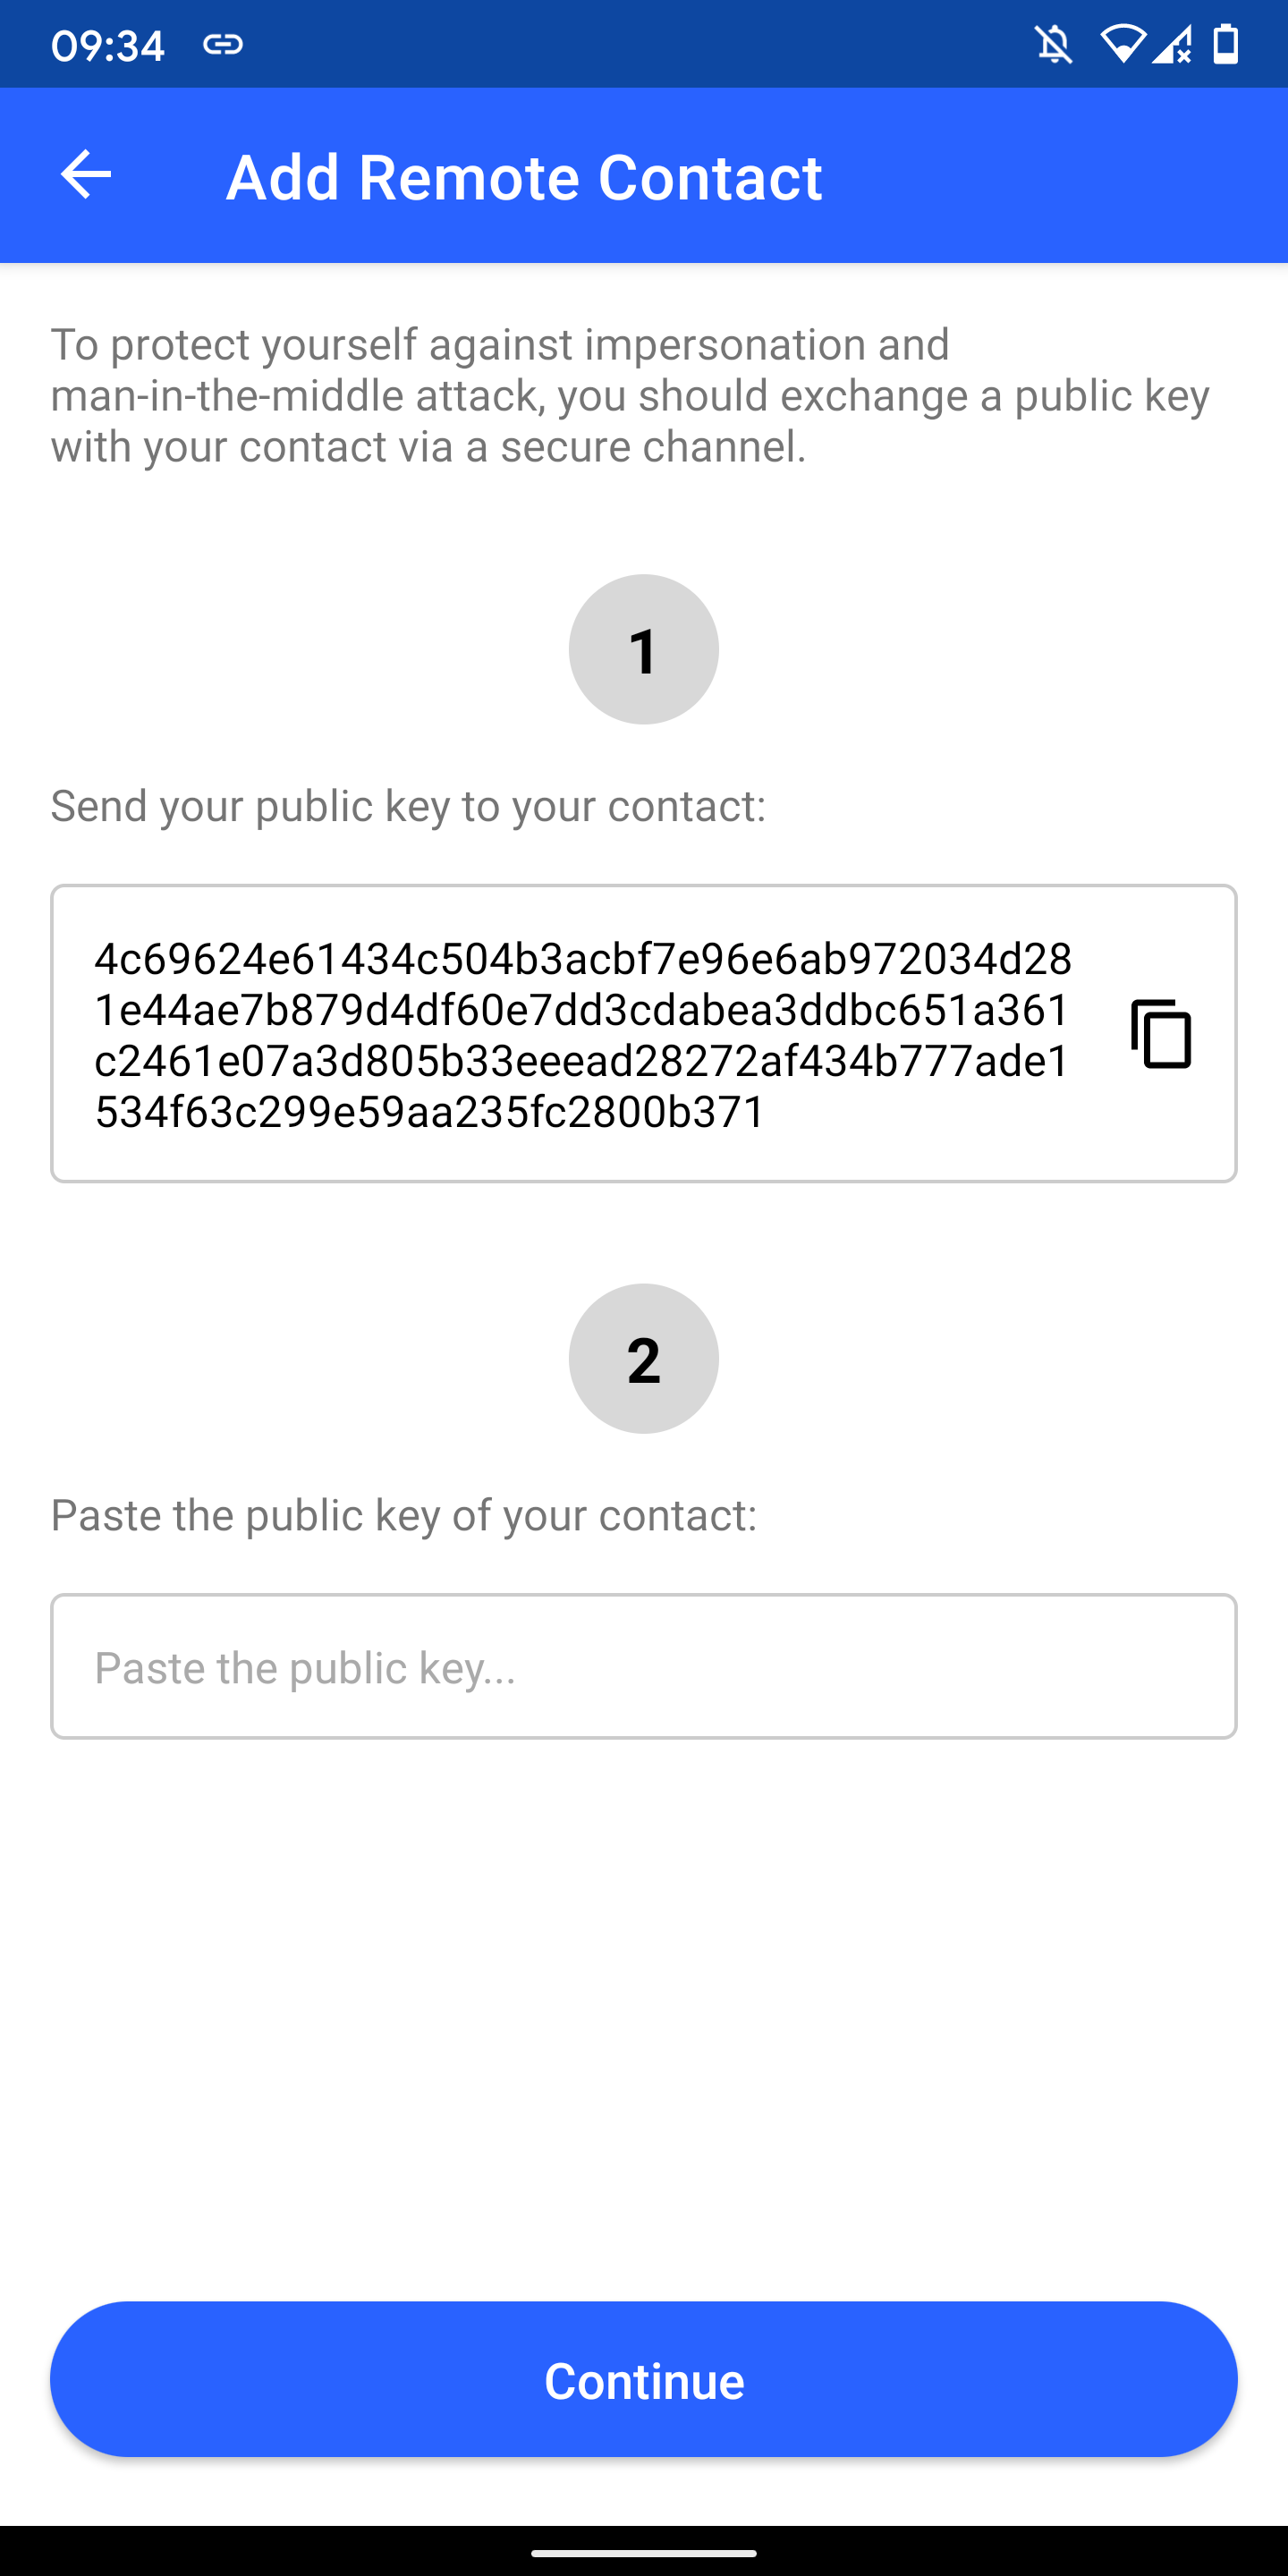
\includegraphics[width=0.32\textwidth]{screens/superapp/add_remote_contact}
    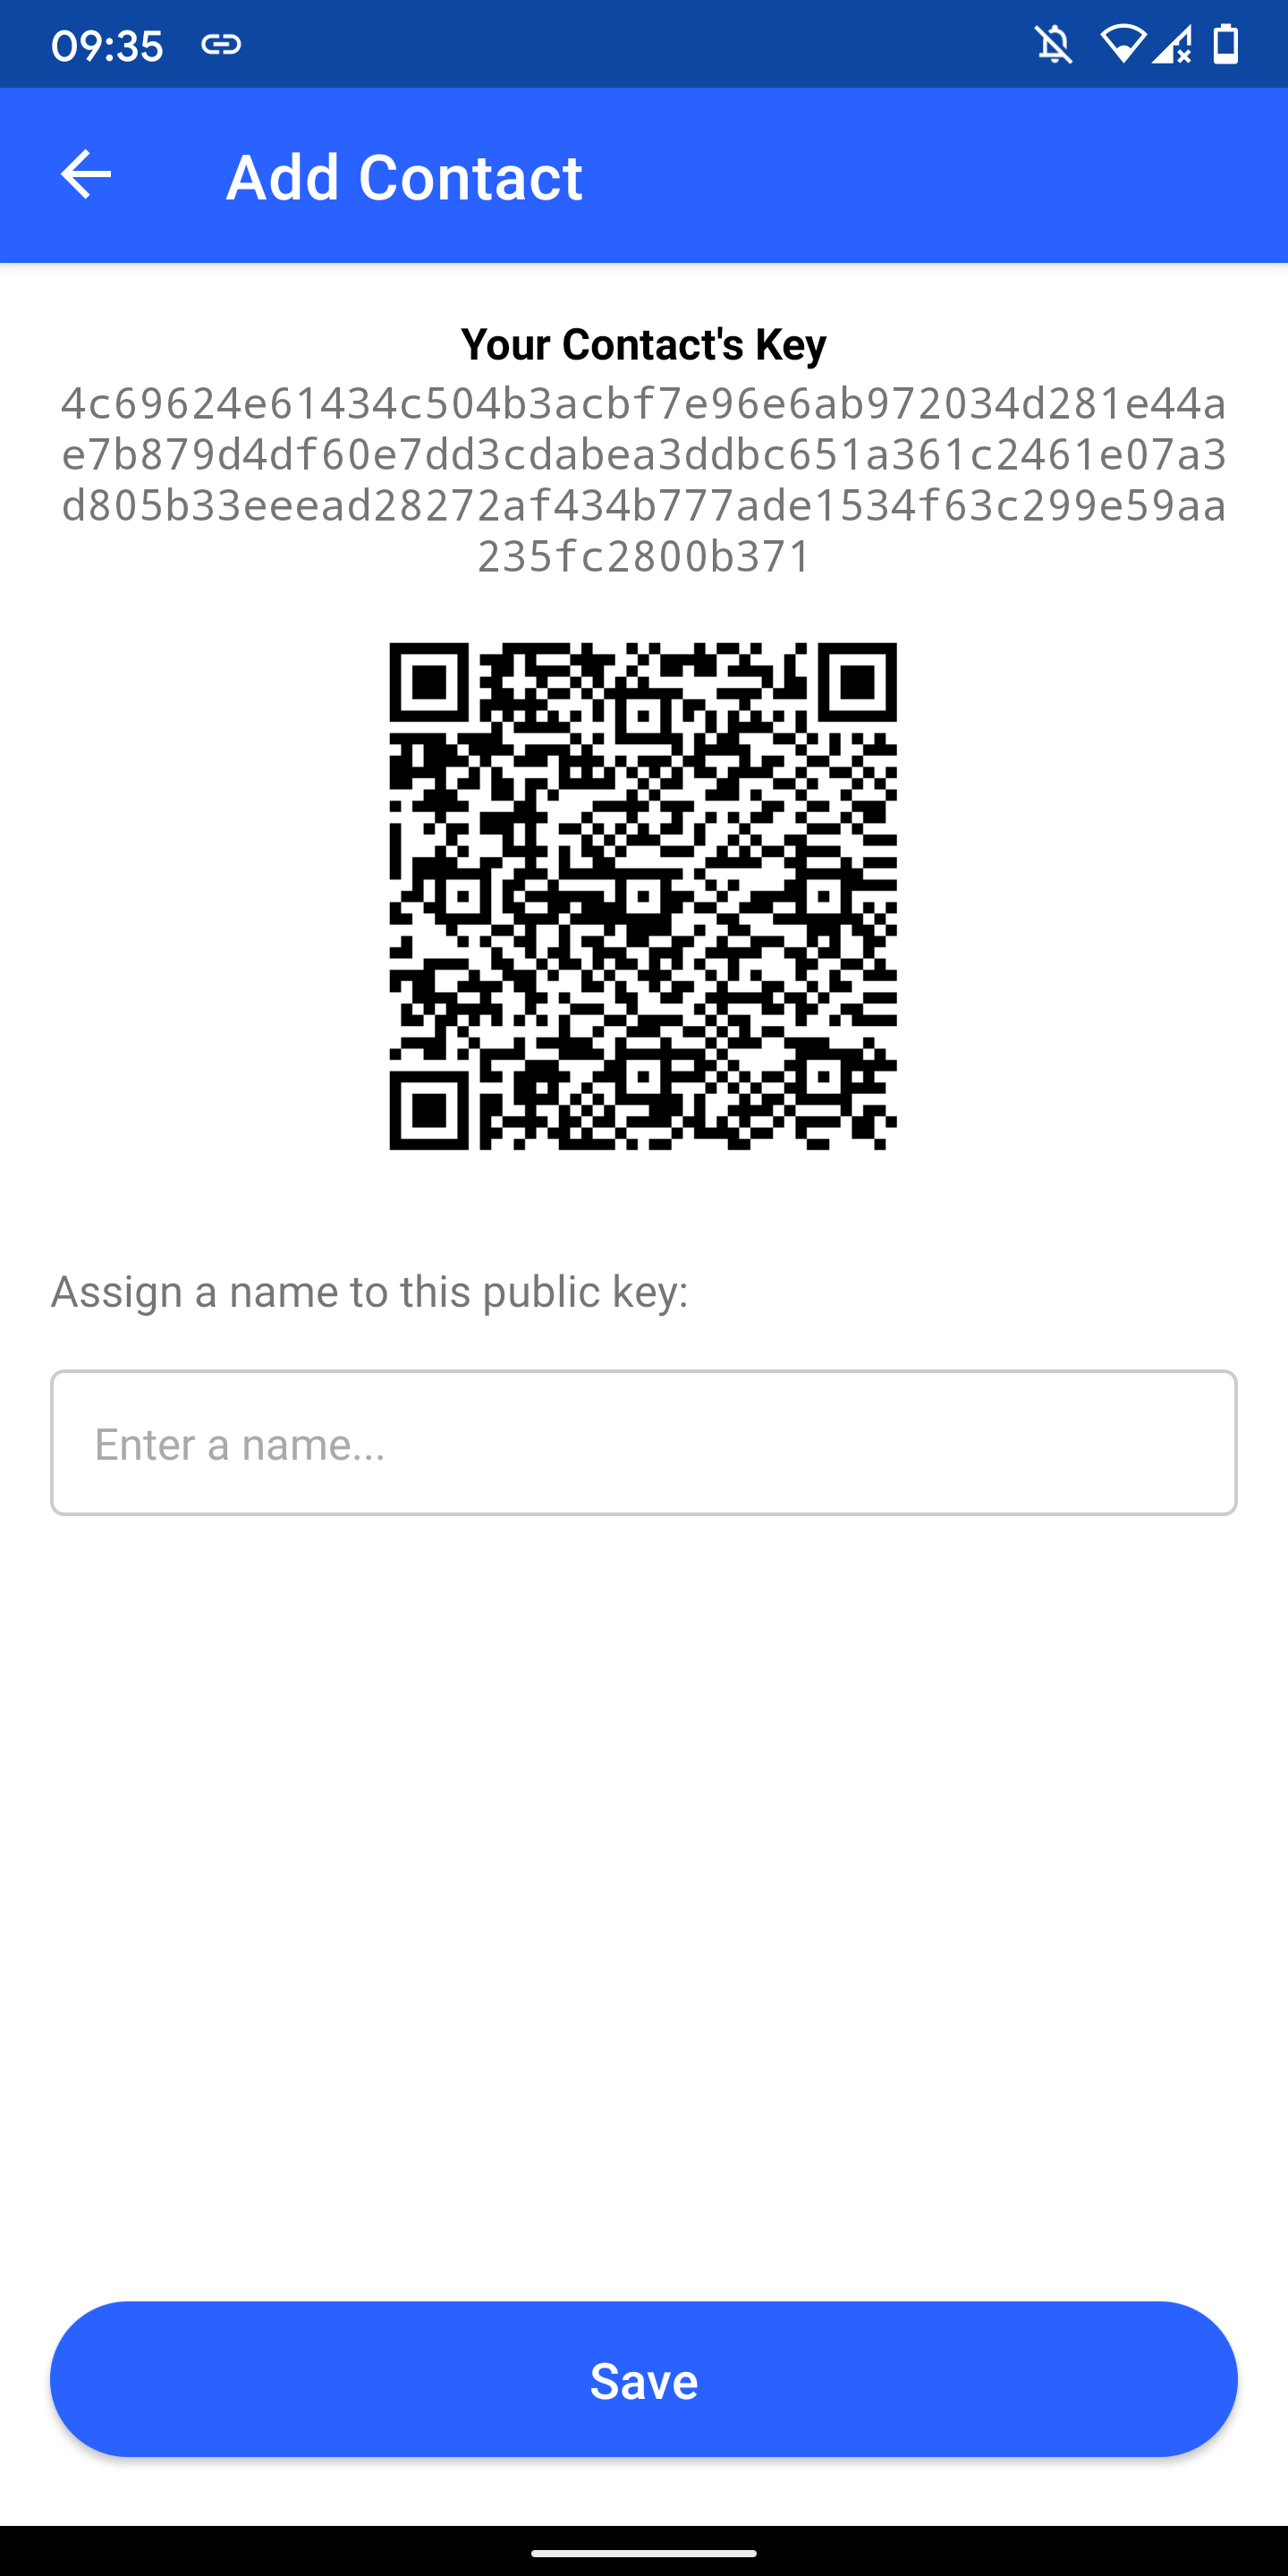
\includegraphics[width=0.32\textwidth]{screens/superapp/add_contact}
    \caption{The UI for adding a public key of a new nearby or remote contact to the trusted public key store, and associating the public key with a human-readable contact name.}
    \label{manyverse}
\end{figure}


\subsection{PeerChat: Private Messaging Protocol}

\begin{figure}
    \centering
    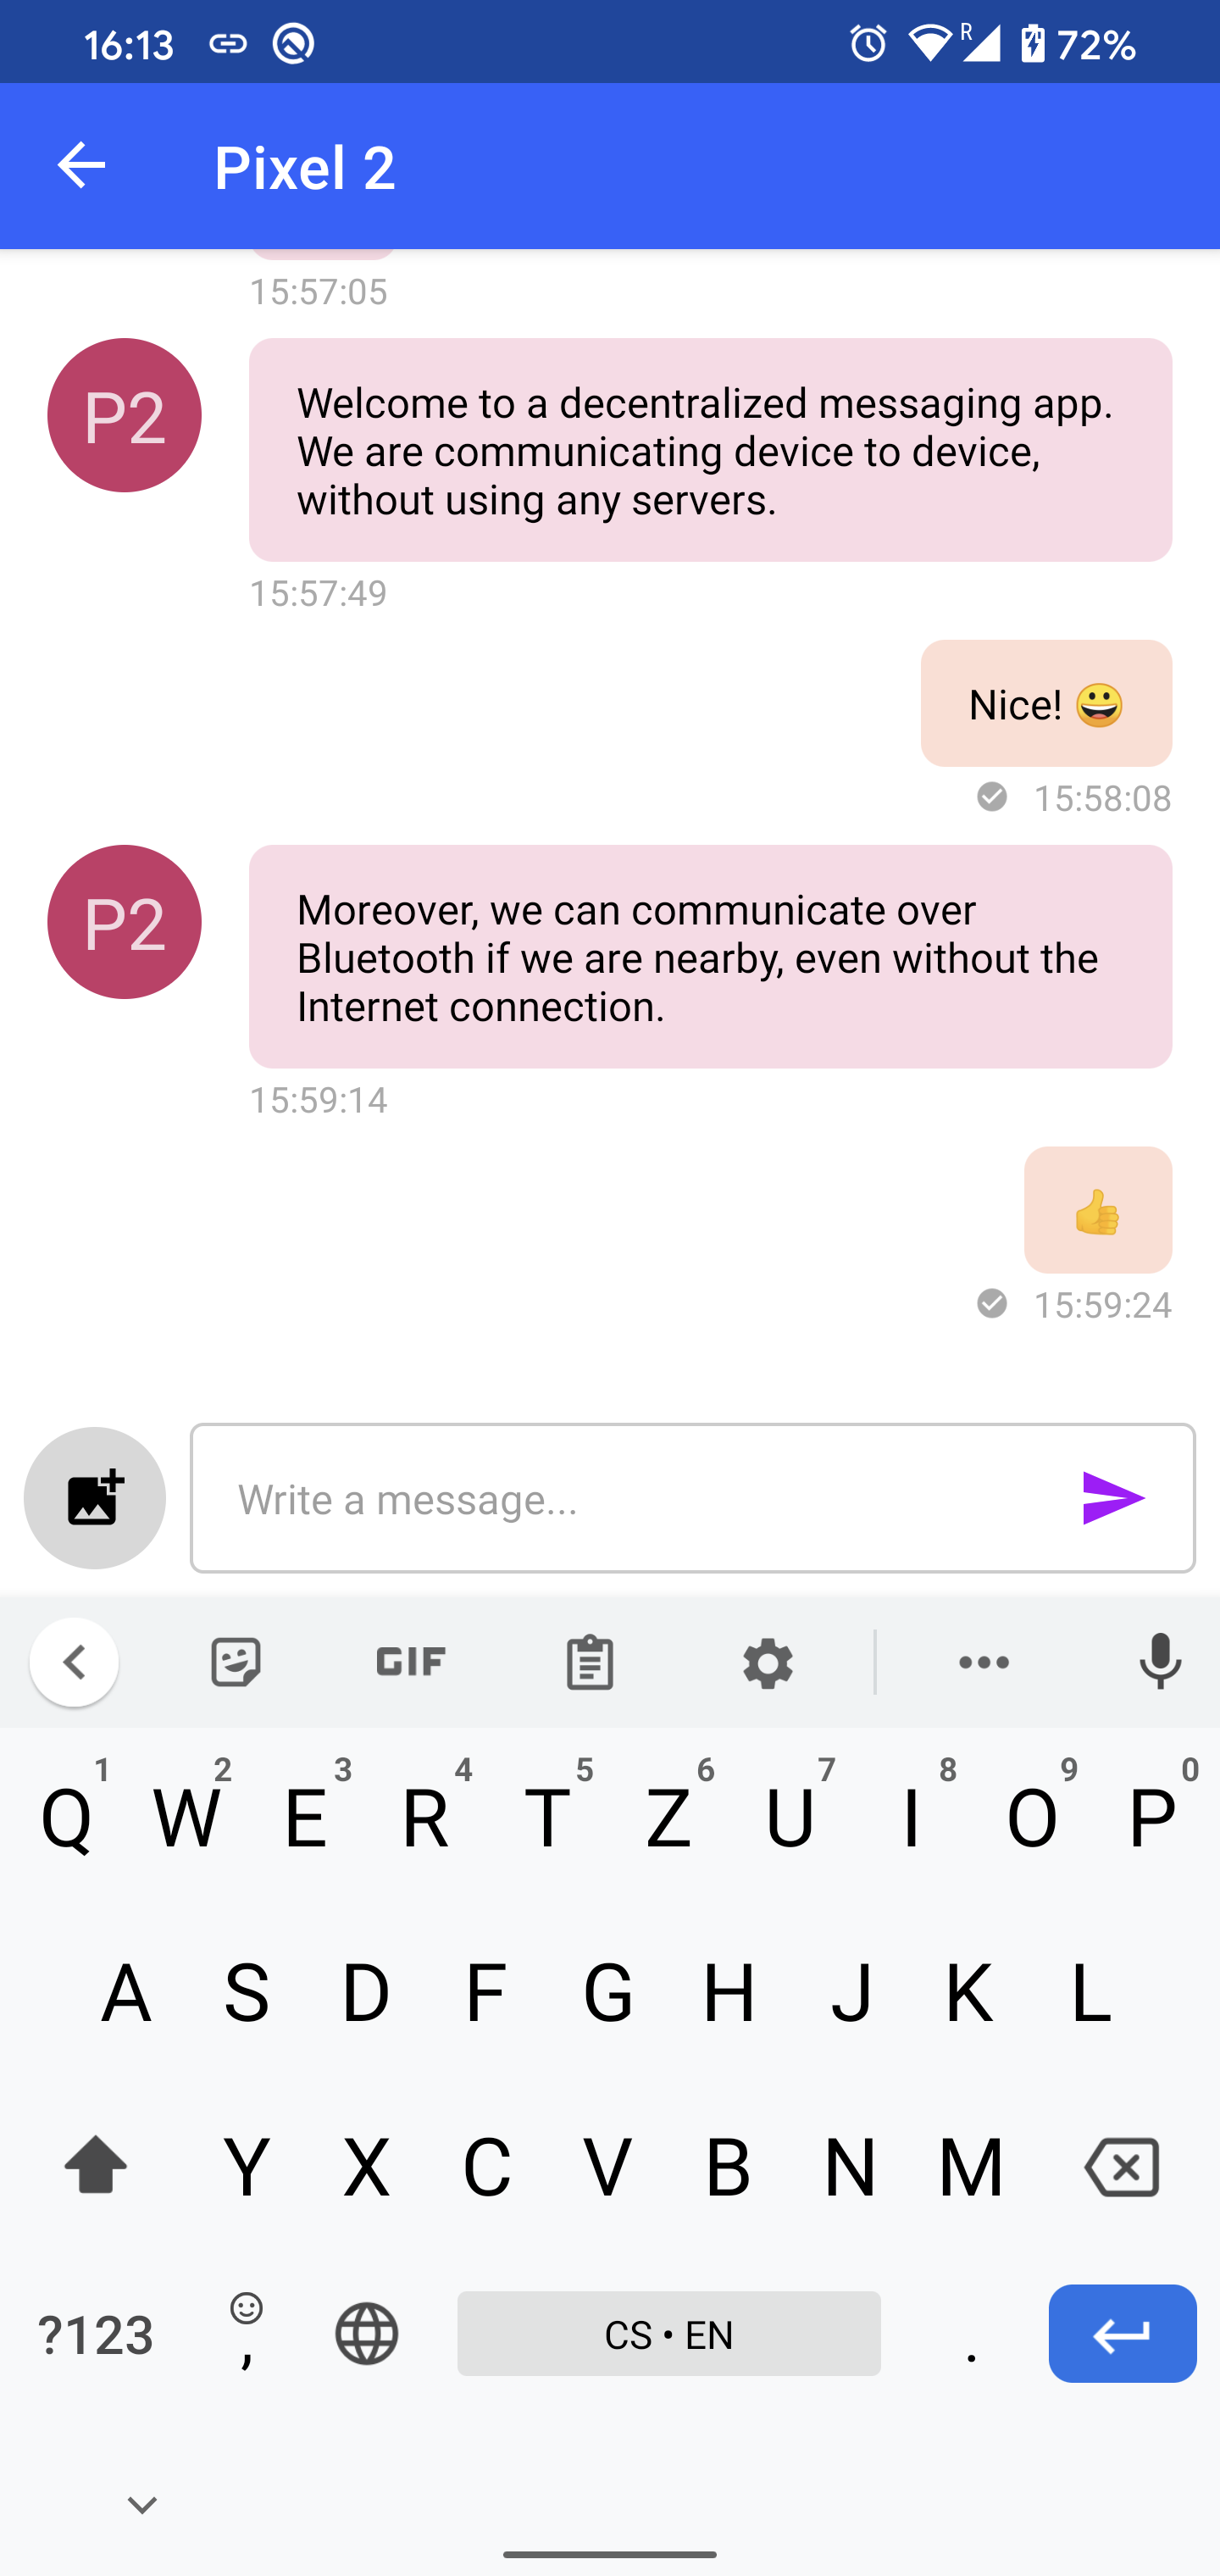
\includegraphics[width=0.32\textwidth]{screens/superapp/conversation_text}
    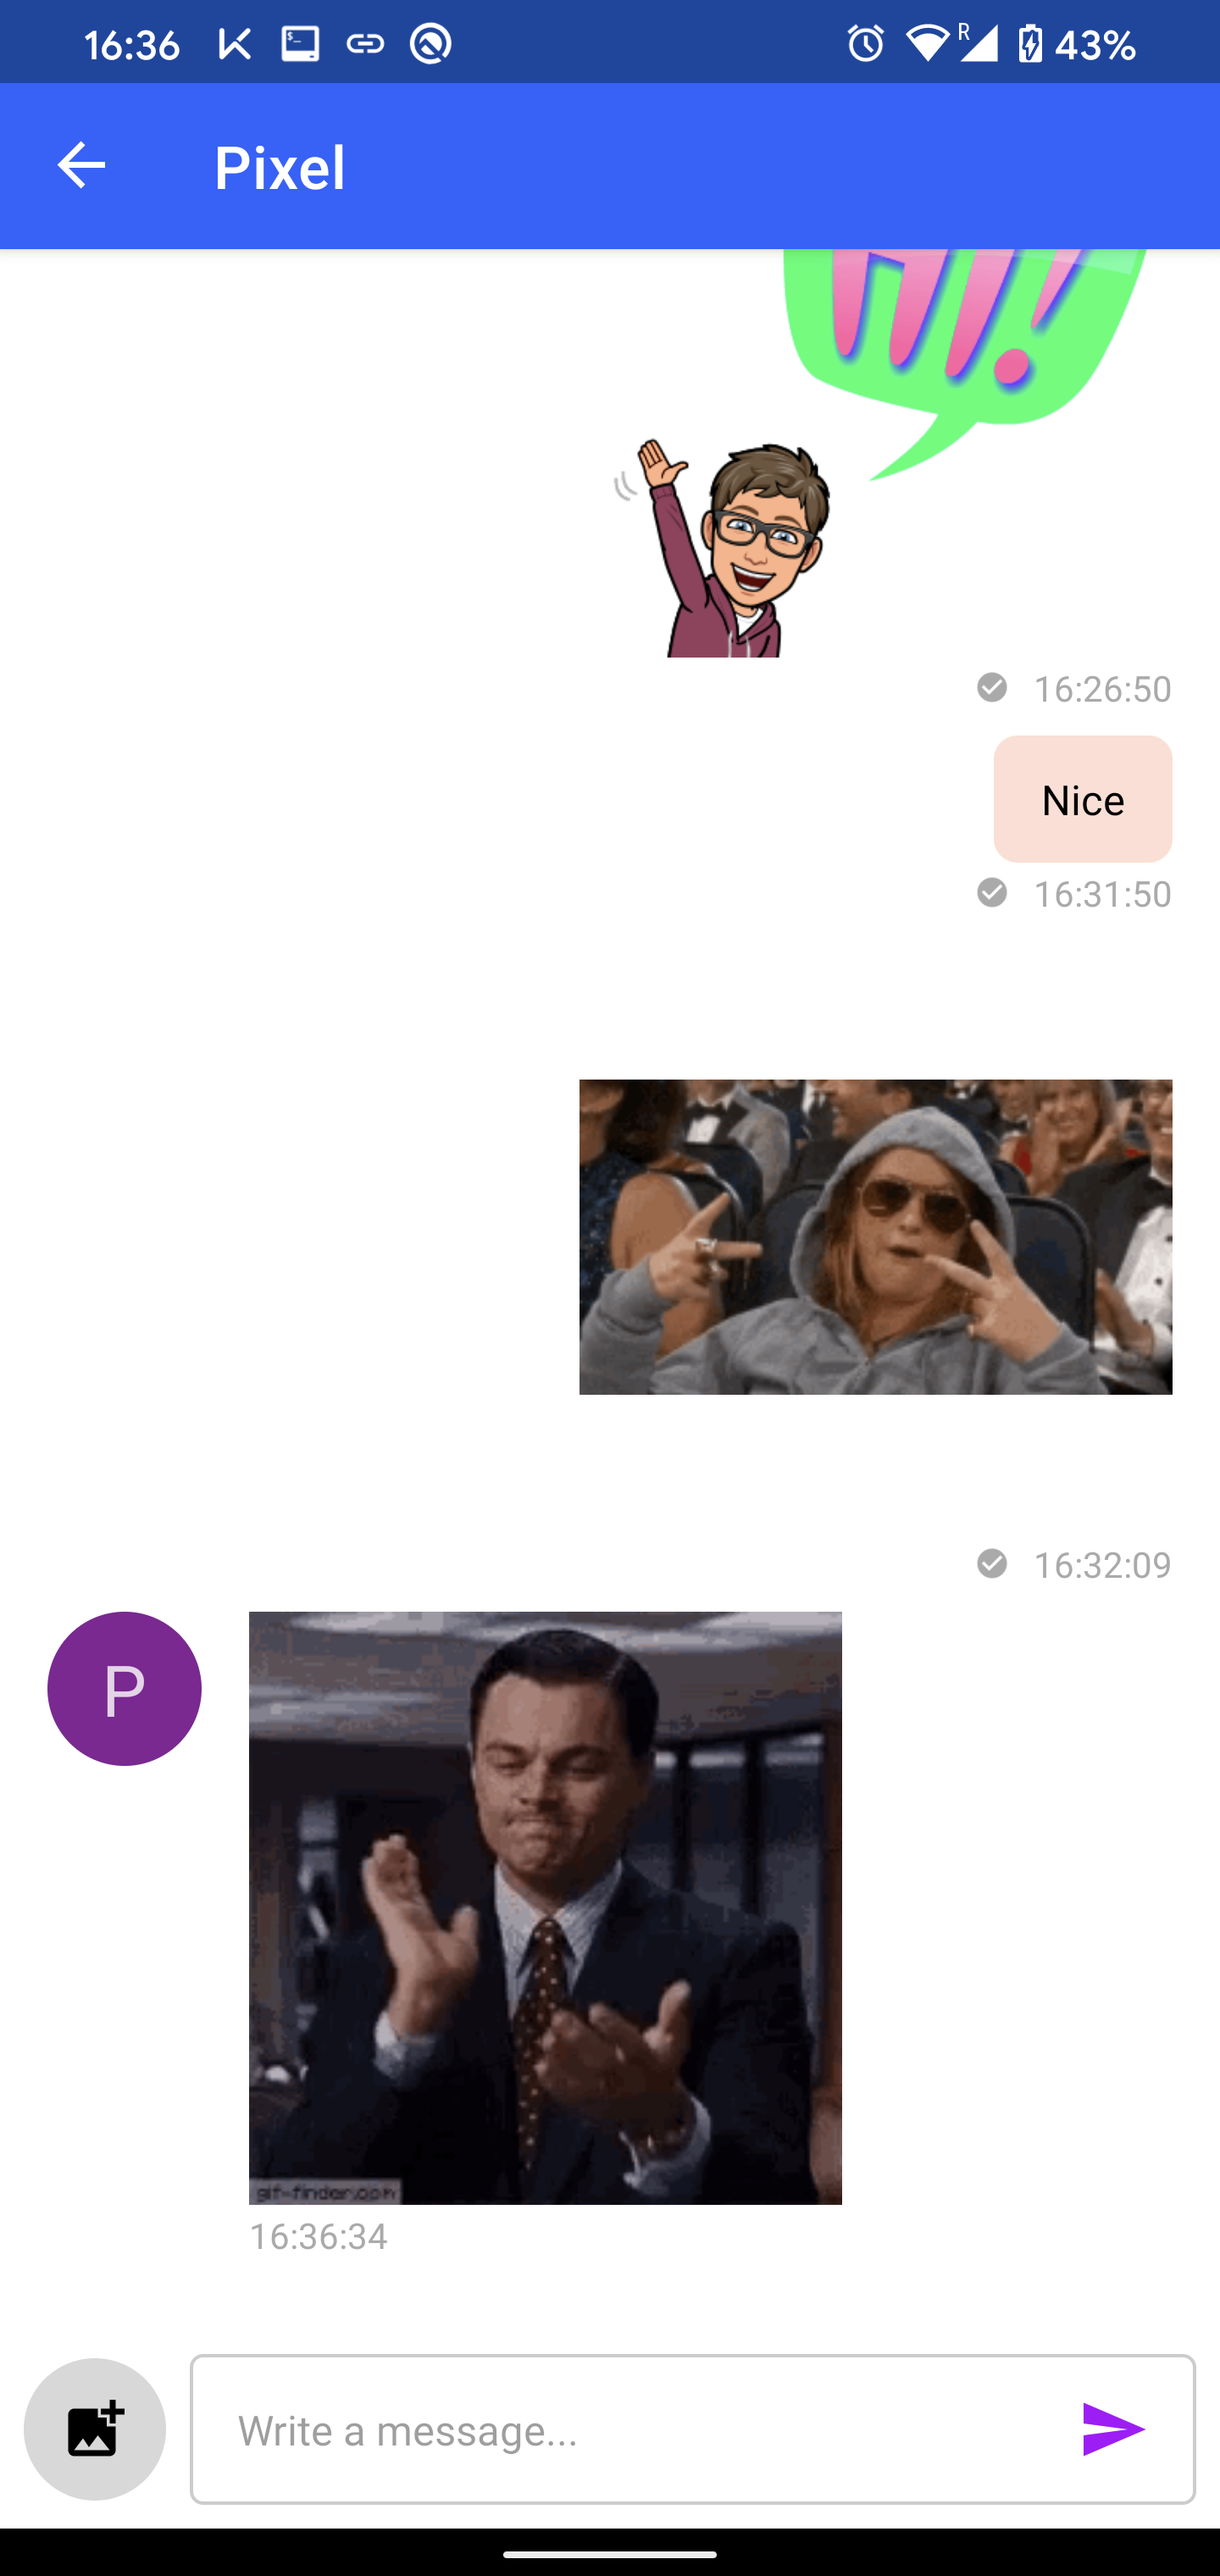
\includegraphics[width=0.32\textwidth]{screens/superapp/conversation}
    \caption{The conversation UI containing incoming and outgoing text messages, image attachments, and delivery indications for outgoing messages.}
    \label{manyverse}
\end{figure}

\subsection{Public Post Feed}

\begin{figure}
    \centering
    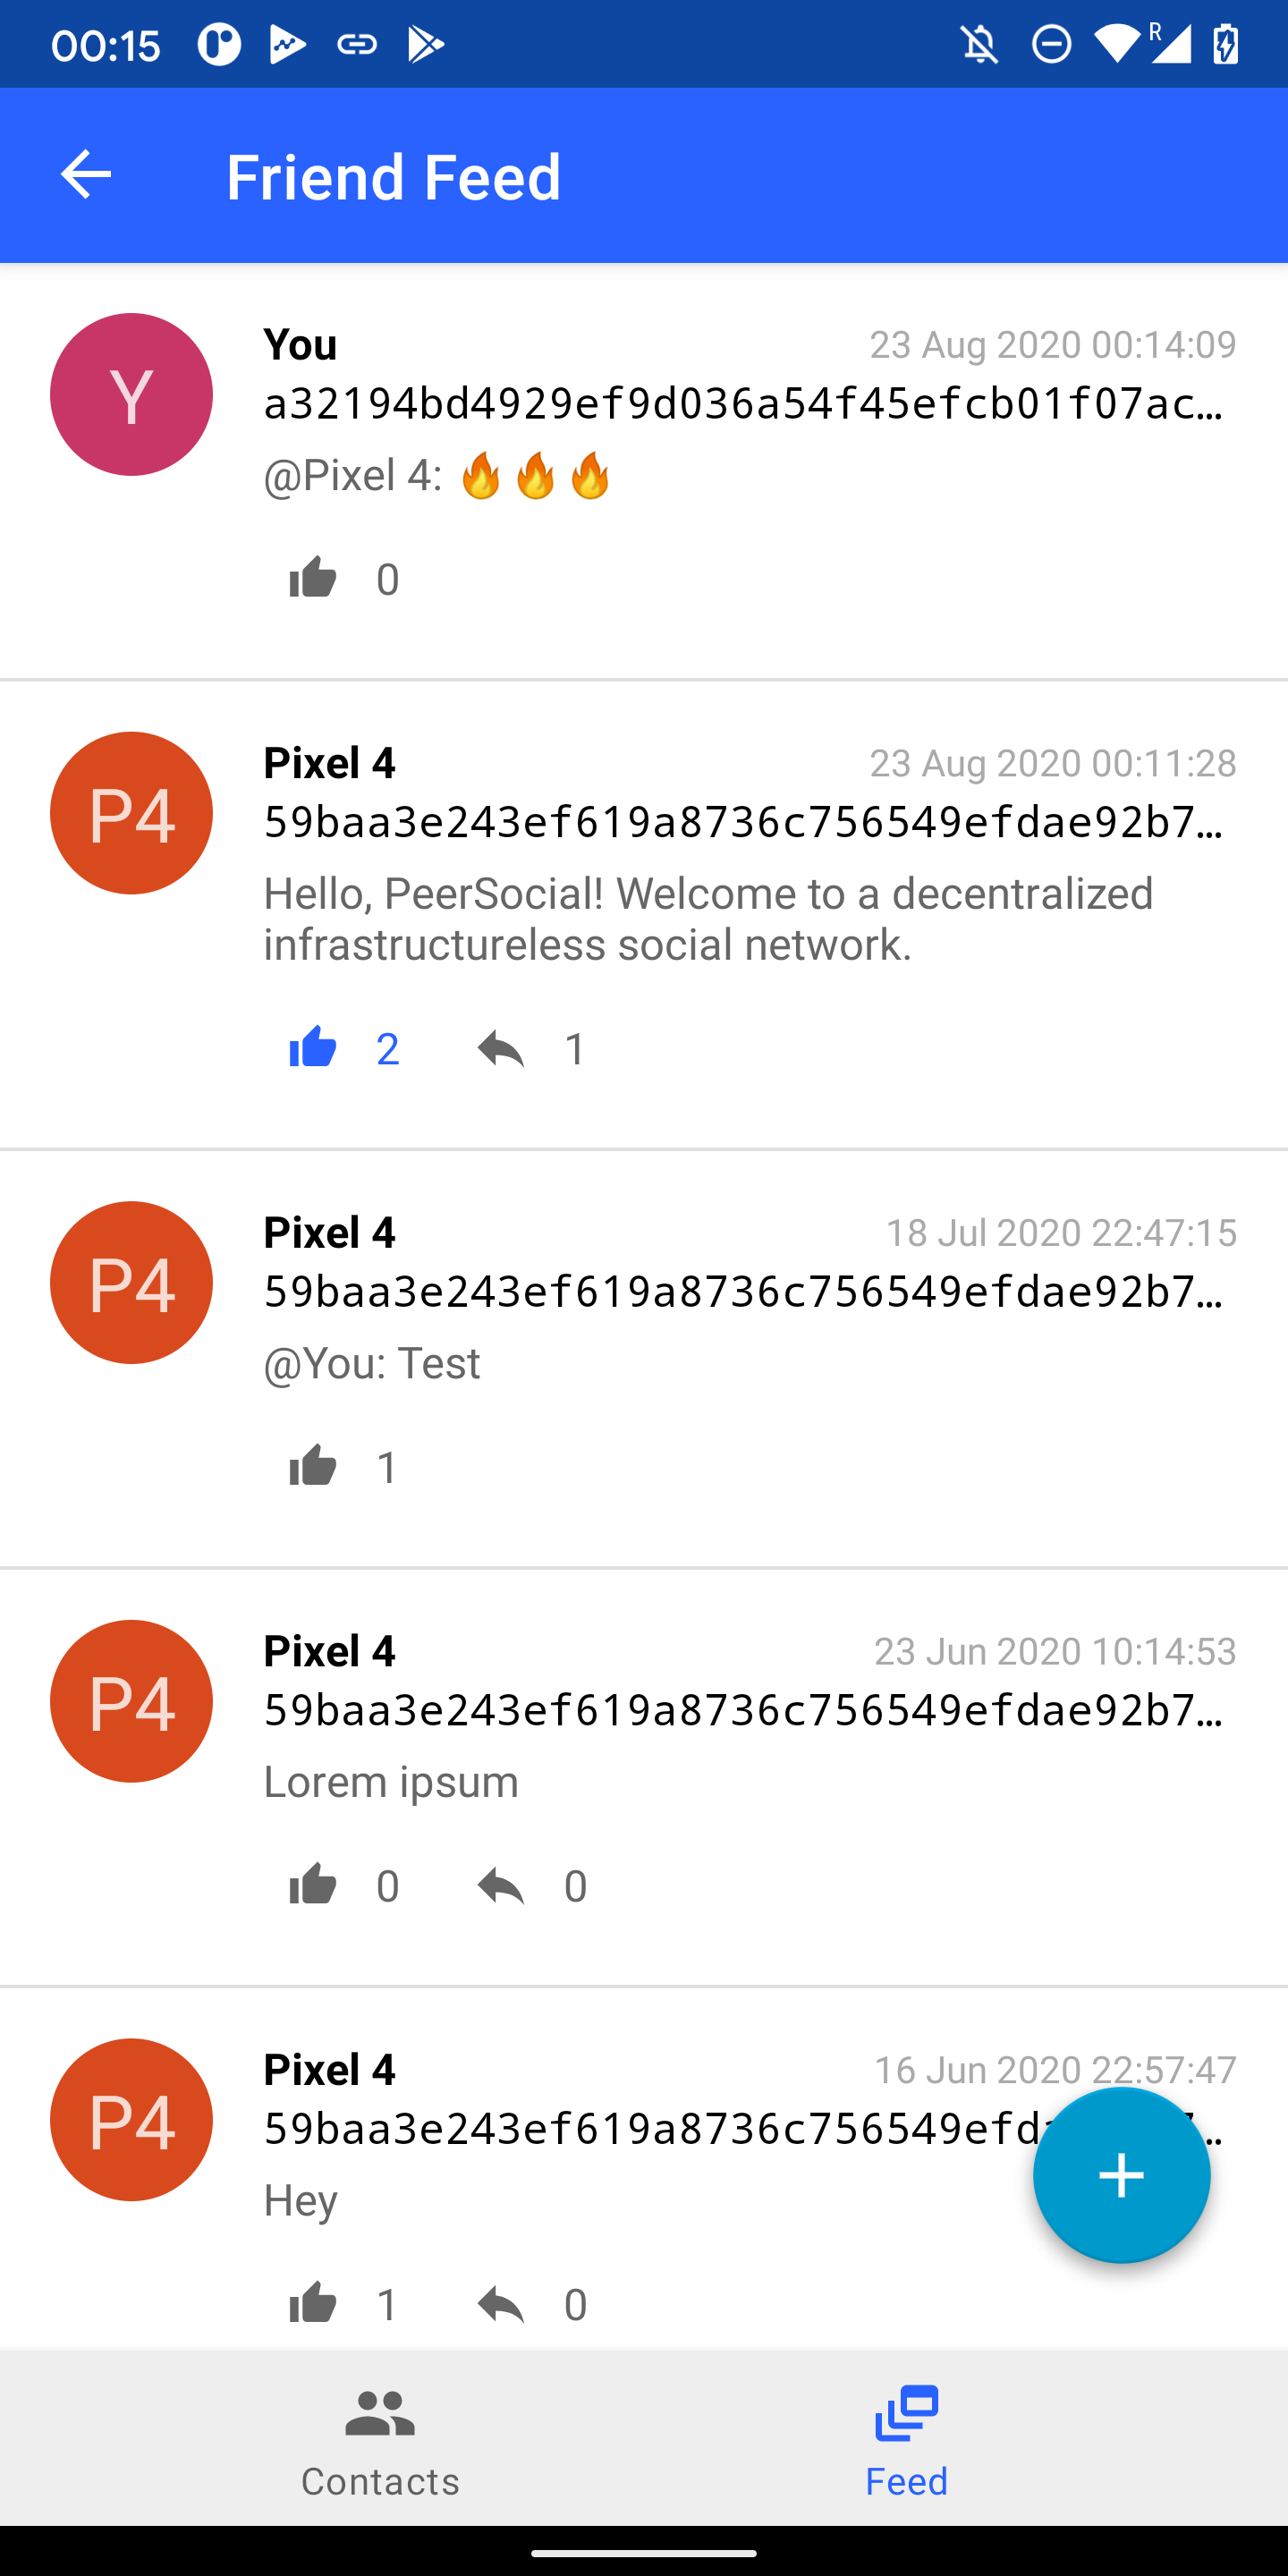
\includegraphics[width=0.32\textwidth]{screens/superapp/feed}
    \caption{The social feed with likes and replies.}
    \label{manyverse}
\end{figure}


%\section{Bluetooth Communication}

%\section{Multi-Transport Routing Algorithm}

%\section{Peer Discovery and Traversal in Distributed Hash Table}

%\section{Packet Format}



%\section{Binary Transfer over UDP}

%\section{Testbed for Distributed Android Applications}

\section{DelftDAO: Framework for Permissionless Economic Activity}

\chapter{Evaluation}

\section{Analysis and Puncturing of Carrier Grade NAT}

According to the report by Statista \cite{statista:marketshare}, there were three major mobile phone operators providing services in the Netherlands in Q4 2018, as listed in Table \ref{table_marketshare}. In total, these represent up to 85 \% of the market share. The rest of the market is shared by Mobile Virtual Network Operators who sell services over existing networks of those three operators.

\begin{table}
    \centering
    \begin{tabular}{ | l | c | }
        \hline
        \textbf{Operator} & \textbf{Market share} \\
        \hline
        \textbf{KPN} & 35\% \\
        \textbf{Vodafone} & 25\% \\
        \textbf{Mobile Virtual Network Operators} & 25\% \\
        \textbf{T-Mobile} & 20\% \\
        \hline
    \end{tabular}
    \caption{Market share of mobile network operators in the Netherlands in Q4 2018. The shares do not sum up to 100\% as they are rounded up within five percent ranges in the original report. \cite{statista:marketshare}}
    \label{table_marketshare}
\end{table}

We have purchased pre-paid SIM cards for all three major mobile network operators to investigate whether they are suitable for peer-to-peer communication. First, we tried to infer the characteristics of their Carrier Grade NAT deployments.

We used the STUN protocol and NAT behavior discovery mechanisms described in \cite{rfc5780}. They have shown that all networks appear to use \textit{Endpoint-Independent Mapping (EIM)} and \textit{Address and Port-Dependent Filtering} (also known as \textit{port-restricted cone NAT}). EIM is a sufficient condition for our NAT traversal mechanism to be successful, so this would make all these NATs suitable for P2P communication.

However, we also observed that NAT behavior of CGN can change over time, so STUN behavior discovery mechanism is not sufficient to correctly classify CGN behavior. We performed some more tests to verify if the behavior is consistent over time. We attempted to connect to 50 different peers over the interval of 5 minutes. We verified that KPN and T-Mobile networks are consistent with EIM behavior. However, the CGNAT used by Vodafone changes the port mapping for new connections approximately every 60 seconds, even when connecting to the same IP address and a different port. While not strictly correct due to temporal dependency, this behavior could be classified as \textit{Address and Port-Dependent Mapping (APDM)} which is characteristic for a \textit{symmetric NAT}.

The mapped ports seem to be assigned at random from the range of 10,000 ports, which makes it infeasible to use any known symmetric NAT traversal techniques such as port prediction or multiple hole punching \cite{multihole}\cite{takeda}.

%The results are presented in Table \ref{table_cgnat_analysis}.


\begin{table}[h!]
    \centering
    \begin{tabular}{ | l | l | l | l | }
        \hline
        \textbf{Operator} & \textbf{Mapping behavior} & \textbf{Filtering behavior} & \textbf{Binding lifetime} \\
        \hline
        \textbf{KPN} & EIM & APDF & ? \\
        \textbf{Vodafone} & EIM, refresh every 60 s & APDF & ? \\
        \textbf{T-Mobile} & EIM & APDF & ? \\
        \hline
    \end{tabular}
    \caption{Characteristics of CGNATs deployed by Dutch mobile network operators}
    \label{table_cgnat_analysis}
\end{table}


% Types of NAT used by different operators
% - T-Mobile - Address-restricted cone
% - Vodafone – symmetric NAT, random port mapping, TODO: analyze port distribution
% - KPN - Address-restricted cone

%\section{Performance Evaluation}

\section{Connectivity Test}

\subsection{Experimental Setup}


\begin{figure}[h!]
    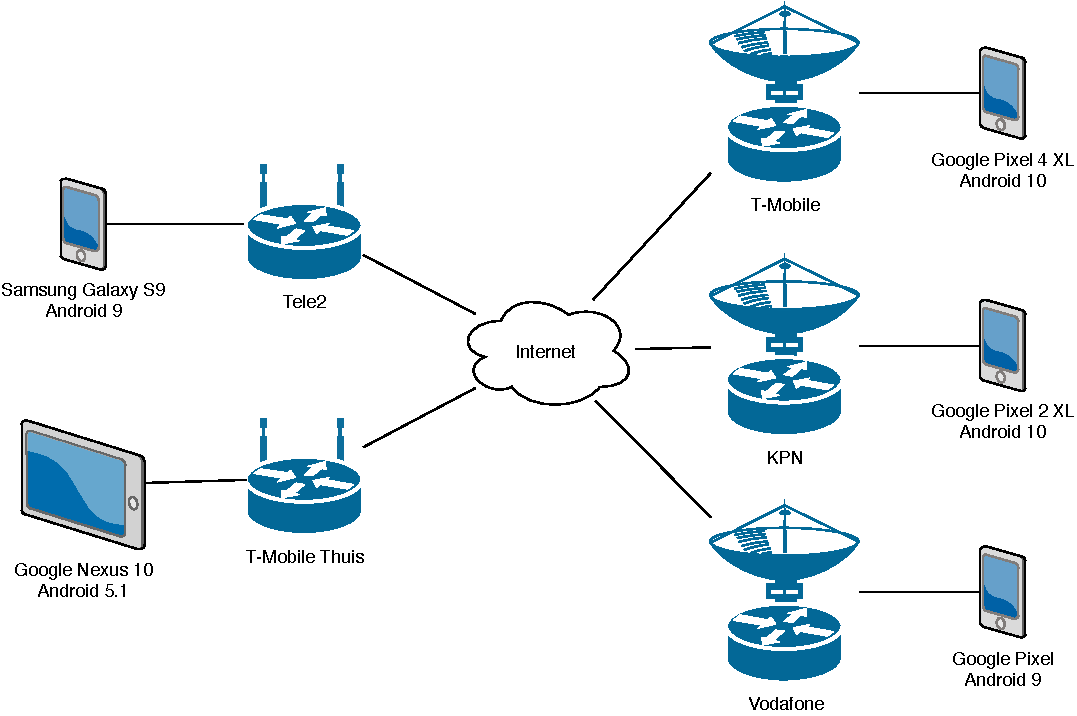
\includegraphics[width=\textwidth]{diagrams/experimental-setup}
    \caption{The experimental setup for the connectivity test using devices connected to different mobile (T-Mobile, KPN, Vodafone) and home broadband (Tele2, T-Mobile Thuis) ISP networks.}
    \label{ble_architecture}
\end{figure}


\subsection{Results}

\begin{table}[h!]
    \centering
    \begin{tabular}{ | l | c | c | c | c | c | }
        \hline
        \textbf{} & \textbf{T-Mobile} & \textbf{KPN} & \textbf{Vodafone} & \textbf{Tele2} & \textbf{T-Mobile Thuis} \\
        \hline
        \textbf{T-Mobile} & \cellcolor{green!25} &  &  &  &  \\
        \hline
        \textbf{KPN} & \cellcolor{green!25}& \cellcolor{green!25} &  &  &  \\
        \hline
        \textbf{Vodafone} & \cellcolor{orange!25} & \cellcolor{green!25} & \cellcolor{yellow!25} &  &  \\
        \hline
        \textbf{Tele2} & \cellcolor{green!25} & \cellcolor{green!25} & \cellcolor{green!25} & \cellcolor{green!25} & \\
        \hline
        \textbf{T-Mobile Thuis} & \cellcolor{green!25} & \cellcolor{green!25} & \cellcolor{green!25} & \cellcolor{green!25} & \cellcolor{green!25} \\
        \hline
    \end{tabular}
    \caption{The connectivity matrix representing the NAT traversal method needed to establish connection between devices connected via different ISPs (green: hole punching, yellow: multihole punching, orange: delayed multihole punching).}
    \label{table_cgnat_analysis}
\end{table}

\section{Bootstrap Performance Evaluation}

\section{Stress Test}

\section{Power Efficiency}

\section{Code Quality}

% experiments:
% - bootstrap from 0 to 20 peers
% - 24-hour stress test


\chapter{Conclusion}

\section{Future Work}
% IPv6 support, multiple network interfaces
% BLE mesh network
% Wi-Fi Aware for higher bandwidth Nearby transfer
% DHT + routing
% WebRTC transport
% multidevice support, key revocation chain
% challenge the super app architecture
% – rather refactor into content provider and split into separate APKs?
% - use React Native for UI?
